% MBDyn (C) is a multibody analysis code.
% http://www.mbdyn.org
%
% Copyright (C) 1996-2005
%
% Pierangelo Masarati  <masarati@aero.polimi.it>
%
% Dipartimento di Ingegneria Aerospaziale - Politecnico di Milano
% via La Masa, 34 - 20156 Milano, Italy
% http://www.aero.polimi.it
%
% Changing this copyright notice is forbidden.
%
% This program is free software; you can redistribute it and/or modify
% it under the terms of the GNU General Public License as published by
% the Free Software Foundation (version 2 of the License).
% 
%
% This program is distributed in the hope that it will be useful,
% but WITHOUT ANY WARRANTY; without even the implied warranty of
% MERCHANTABILITY or FITNESS FOR A PARTICULAR PURPOSE.  See the
% GNU General Public License for more details.
%
% You should have received a copy of the GNU General Public License
% along with this program; if not, write to the Free Software
% Foundation, Inc., 59 Temple Place, Suite 330, Boston, MA  02111-1307  USA

\documentclass[10pt,dvips]{report}

%\usepackage[pdftex]{graphicx}
\usepackage[T1]{fontenc}
\usepackage{ae,aecompl}
\usepackage{graphicx}
\usepackage{psfrag}
\usepackage{amsmath}
\usepackage[dvips,breaklinks=true,colorlinks=false]{hyperref}
\usepackage{html}

% $Header$
% Copyright (C) 1996-2015 Pierangelo Masarati <masarati@aero.polimi.it>
% Dipartimento di Ingegneria Aerospaziale, Politecnico di Milano
%
% Parentesi: tonde, quadre, curly, dritte, doppie e angolari.
\newcommand{\plbr}[1]{ \left( #1 \right) }
\newcommand{\sqbr}[1]{ \left[ #1 \right] }
\newcommand{\cubr}[1]{ \left\{ #1 \right\} }
\newcommand{\shbr}[1]{ \left| #1 \right| }
\newcommand{\nrbr}[1]{ \left\| #1 \right\| }
\newcommand{\anbr}[1]{ \langle #1 \rangle }

% Parentesi solo a sinistra: tonde, quadre, curly, dritte, doppie e angolari.
\newcommand{\lplbr}[1]{ \left( #1 \right. }
\newcommand{\lsqbr}[1]{ \left[ #1 \right. }
\newcommand{\lcubr}[1]{ \left\{ #1 \right. }
\newcommand{\lshbr}[1]{ \left| #1 \right. }
\newcommand{\lnrbr}[1]{ \left\| #1 \right. }
\newcommand{\lanbr}[1]{ \langle #1 \right. }

% Parentesi solo a destra: tonde, quadre, curly, dritte,doppie e angolari.
\newcommand{\rplbr}[1]{ \left. #1 \right) }
\newcommand{\rsqbr}[1]{ \left. #1 \right] }
\newcommand{\rcubr}[1]{ \left. #1 \right\} }
\newcommand{\rshbr}[1]{ \left. #1 \right| }
\newcommand{\rnrbr}[1]{ \left. #1 \right\| }
\newcommand{\ranbr}[1]{ \left. #1 \rangle }

% Vettori verticali:
\newcommand{\vvect}[2]{ \begin{array}{ #1 } #2 \end{array} }
\newcommand{\cvvect}[1]{ \begin{array}{c} #1 \end{array} }
\newcommand{\lvvect}[1]{ \begin{array}{l} #1 \end{array} }
\newcommand{\rvvect}[1]{ \begin{array}{r} #1 \end{array} }

% Vettori orizzontali:
\newcommand{\hvect}[2]{ \begin{array}{ #1 } #2 \end{array} }

% Matrici:
\newcommand{\matr}[2]{ \begin{array}{ #1 } #2 \end{array} }

% Integrali: uso \intg{inf}{sup}{arg}{dvar}
\newcommand{\intg}[4]{ \int_{#1}^{#2} {#3} \ {#4} }

% Limite: uso \limt{var}{lim}{arg}
\newcommand{\limt}[3]{ \lim_{{#1} \rightarrow {#2}} {#3}}

% LogLike functions
\newcommand{\llk}[1]{\ensuremath{\mathrm{#1}}}

\newcommand{\diag}[0]{\llk{diag}}
\newcommand{\tr}[0]{\llk{tr}}
\newcommand{\sym}[0]{\llk{sym}}
\newcommand{\skw}[0]{\llk{skw}}

\newcommand{\step}[0]{\llk{step}}
\newcommand{\imp}[0]{\llk{imp}}

\newcommand{\grad}[0]{\llk{grad}}
\newcommand{\divr}[0]{\llk{div}}
\newcommand{\rot}[0]{\llk{rot}}

% In italiano ...
\newcommand{\sca}[0]{\llk{sca}}

% first, second, etc
\newcommand{\first}[0]{1\ensuremath{^{\mathrm{st}}}}    % 1^st
\newcommand{\second}[0]{2\ensuremath{^{\mathrm{nd}}}}   % 2^nd
\newcommand{\third}[0]{3\ensuremath{^{\mathrm{rd}}}}    % 3^rd
\newcommand{\rth}[0]{\ensuremath{^{\mathrm{th}}}}       %  ^th

\newcommand{\degr}[0]{\ensuremath{^{\mathrm{o}}}}

% esponenziale
\providecommand{\e}[1]{\llk{e}^{#1}}


\newcommand{\kw}[1]{\texttt{#1}}
%\newcommand{\kw}[1]{\fbox{\texttt{#1}}}
\newcommand{\T}[1]{\boldsymbol{#1}}

% Custom
\topmargin 0.31cm % 0.00cm
\oddsidemargin 0.00cm
\evensidemargin 0.00cm
\marginparsep 0.00cm
\textwidth 15.92cm
\textheight 23.00cm % 23.62cm

\begin{document}

\begin{latexonly}
\title{\bf MBDyn Input File Format \\
Version
\input{../build/version}
}
\author{Pierangelo Masarati \vspace{5mm}\\
    \sc Dipartimento di Ingegneria Aerospaziale \\
    \sc Politecnico di Milano}
\date{Automatically generated \today}
\maketitle
\end{latexonly}

\begin{htmlonly}
\begin{center}
\textbf{\LARGE MBDyn Input File Format}

\emph{\large Pierangelo Masarati}

\textsc{Dipartimento di Ingegneria Aerospaziale \\ Politecnico di Milano}

\today
\end{center}
\end{htmlonly}

\tableofcontents
\newpage
\listoffigures
\newpage
\listoftables
\newpage

\chapter*{Introduction}
This document describes the format of the input data for MBDyn,
the \underline{M}ulti\underline{b}ody \underline{Dyn}amics analysis suite.
It should be considered a syntax more than a format, since the rules of the
input allow a lot of freedom in the file format. 

\section*{Conventions on the Notation}
throughout the manual, a (sometimes na\"{\i}ve) 
Backus-Naur-like syntax description is used. 
Extensions are made, such as to put extra arguments in square brackets
\kw{[]}, mutually exclusive arguments in curl brackets \kw{\{\}},
separated by the logical ``or'' \kw{|} operator.
Non-terminal symbols are enclosed in angle brackets \kw{<>}, while
terminal symbols are written in normal types.
The association of a non-terminal with terminal or non-terminal
symbols is performed by means of the operator `\kw{::=}'. 
% Special characters are enclosed in simple quotes \kw{`}, and \kw{'}.
When required, the type of a non-terminal symbol is enforced in a ``C''
programming language casting style, by prepending a (usually
self-explanatory) type enclosed in plain brackets \kw{()}.


\section*{Remarks}
The input of the program MBDyn is subject to continuous changes
at a fast pace, since the code is under development.
This documentation attempts to give some insight into the logics 
that drove its implementation.
While most of the software resulted from a careful design, 
some portions are ``as they are'' only because they were made in a hurry, 
or because no better way was at hand at the moment they were made.
The input format partially reflects the development of the software.
Whenever changes in the input format and in the syntax 
of existing parts are required, an effort will be attempted to make 
it as much backward compatible as possible, or at least reliable 
diagnostics and error checking will be put in place that warns 
for possible erroneous inputs related to a change in the input format. 
At present the input of MBDyn already warns for many possible errors 
and makes as many cross-checks as possible on the consistency of the data. 
Nearly every warning and error issue shows the line of the input file 
where the error occurred. 
Since at present multiple files can be scanned by means of the 
\kw{include} directive, the file where the error occurred
may not be clearly indicated if no reliable C++ exception handling 
is supported by the compiler.
This document will be subjected to changes, so be sure you always have 
a release that is aligned with the version of the code you're running.

For any question or problem, to fix typos, bugs, for comments and
suggestions, please contact the Development Team
without hesitation:\vspace{10mm}\\

\noindent
\begin{tabular}{ll}
\multicolumn{2}{l}{Pierangelo Masarati,} \\
\multicolumn{2}{l}{MBDyn Development Team} \\
\multicolumn{2}{l}{Dipartimento di Ingegneria Aerospaziale} \\
\multicolumn{2}{l}{Politecnico di Milano} \\
\multicolumn{2}{l}{via La Masa 34, 20156 Milano, Italy} \\
Fax: & +39 02 2399 8334 \\
E-mail: & \htmladdnormallink{\kw{mbdyn@aero.polimi.it}}{mailto:mbdyn@aero.polimi.it} \\
Web: & \htmladdnormallink{\kw{http://www.aero.polimi.it/\~{}mbdyn/}}{http://www.aero.polimi.it/~mbdyn/}
\end{tabular}
\vspace{10mm}


\noindent
This manual is also available online at \\
\htmladdnormallink{\kw{http://mbdyn.aero.polimi.it/\~{}masarati/MBDyn-input/manual/index.html}}{http://mbdyn.aero.polimi.it/~masarati/MBDyn-input/manual/index.html}


% $Header$
% MBDyn (C) is a multibody analysis code.
% http://www.mbdyn.org
%
% Copyright (C) 1996-2011
%
% Pierangelo Masarati  <masarati@aero.polimi.it>
%
% Dipartimento di Ingegneria Aerospaziale - Politecnico di Milano
% via La Masa, 34 - 20156 Milano, Italy
% http://www.aero.polimi.it
%
% Changing this copyright notice is forbidden.
%
% This program is free software; you can redistribute it and/or modify
% it under the terms of the GNU General Public License as published by
% the Free Software Foundation (version 2 of the License).
% 
%
% This program is distributed in the hope that it will be useful,
% but WITHOUT ANY WARRANTY; without even the implied warranty of
% MERCHANTABILITY or FITNESS FOR A PARTICULAR PURPOSE.  See the
% GNU General Public License for more details.
%
% You should have received a copy of the GNU General Public License
% along with this program; if not, write to the Free Software
% Foundation, Inc., 59 Temple Place, Suite 330, Boston, MA  02111-1307  USA

\chapter{Overview}\label{sec:OVERVIEW}
This chapter gives a global overview of the structure of the input file.


\section{Input File Structure}
The input is divided in blocks.
This is a consequence of the fact that almost every module of the code 
needs data and each module is responsible for its data input. 
So it is natural to make each module read and interpret its data starting 
from the input phase.

Every statement (or `card') follows the syntax:
%\begin{verbatim}
\begin{Verbatim}[commandchars=\\\{\}]
    \bnt{card} ::= \bnt{description} [ : \bnt{arglist} ] ;
\end{Verbatim}
%\end{verbatim}
\nt{arglist} is a(n optional) list of arguments, that is driven by the 
\nt{description} that identifies the card. 
The keyword can be made of multiple words separated by spaces or tabs; 
the extra spaces\footnote{
	Anything that makes the C function \texttt{isspace()} 
	return \kw{true}
} are skipped, and the match is case insensitive. 
The arguments are usually separated by commas\footnote{
	A few exceptions require a colon to separate blocks of arguments;
	wherever it is feasible, those exceptions will be eliminated 
	in future versions.
	Those cards will be marked as deprecated.
}.
A semicolon ends the card. 

Many cards allow extra arguments that may assume default values 
if not supplied by the user. 
Usually these arguments are at the end of the card
and must follow some rules. 
A check for the existence of extra args is made,
and they are usually read in a fixed sequence.
Optional args are usually prefixed by a keyword.

When structured arguments like matrices, vectors, or drive callers are
expected, they are parsed by dedicated functions.
Anyway, the structured data always follows the rules of the general data. 
Few exceptions are present, and will be eliminated soon.
Every data block is surrounded by the control statements \kw{begin} and
\kw{end}:
%\begin{verbatim}
\begin{Verbatim}[commandchars=\\\{\}]
    \kw{begin} : \bnt{block_name} ;
        # block content
    \kw{end} : \bnt{block_name} ;
\end{Verbatim}
%\end{verbatim}
The block sequence is:
%\begin{verbatim}
\begin{Verbatim}[commandchars=\\\{\}]
    \kw{begin} : \kw{data} ;
        # select a problem
        \kw{problem} : \bnt{problem_name} ;
    \kw{end} : \kw{data} ;

    \kw{begin} : \bnt{problem_name} ;
        # problem-specific data
    \kw{end} : \bnt{problem_name} ;

    \kw{begin} : \kw{control data} ;
        # model control data
    \kw{end} : \kw{control data} ;

    \kw{begin} : \kw{nodes} ;
        # nodes data
    \kw{end} : \kw{nodes} ;

    # note: optional, if requested in \kw{control data}
    \kw{begin} : \kw{drivers} ;
        # special drivers data
    \kw{end} : \kw{drivers} ;

    \kw{begin} : \kw{elements} ;
        # elements data
    \kw{end} : \kw{elements} ;
\end{Verbatim}
%\end{verbatim}
The \kw{drivers} block is optional.

The Schur solver allows an extra block after that of the elements:
%\begin{verbatim}
\begin{Verbatim}[commandchars=\\\{\}]
    # note: optional; only allowed when Schur solver is defined in \nt{problem_name}
    \kw{begin} : \kw{parallel} ;
        # parallel data
    \kw{end} : \kw{parallel} ;
\end{Verbatim}
%\end{verbatim}
where data specific to the partitioning and the connectivity
of the Schur solver is provided.
This is yet undocumented, and will likely be described 
in a future chapter.

Chapter~\ref{sec:GENERAL} describes the basic and aggregate
data structures that concur in building up the cards.
Chapter~\ref{sec:DATA} describes problem selection options.
Chapter~\ref{sec:PROBLEMS} describes the cards dedicated
to the specification of the parameters of the simulation
and of the selected integration scheme.
Chapter~\ref{sec:CONTROL-DATA} describes the model control data.
Chapter~\ref{sec:NODES} describes the cards related to the input
of nodes.
Nodes come first because they are the elementary blocks 
of the connectivity graph of the model, so historically 
they had to be defined before any element could be introduced.
Chapter~\ref{sec:DRIVERS} describes the cards related 
to special drivers.
Chapter~\ref{sec:ELEMENTS} describes the cards related to the input
of elements.



\section{Output}
The program outputs data to a set of files for each simulation.
The contents of each file is related to the file extension,
which is appended to the input file if no output file name 
is explicitly supplied.

If no input file is explicitly provided as well, and thus input
is directly read from \kw{stdin}, the output file name defaults
to `MBDyn'.
Otherwise, unless the output file name is explicitly set, the name 
of the input file is used.

The contents of the output files are described within the description
of the items (nodes or elements) that generate them.
Only a general information file, with extension \texttt{.out}, 
is described here. 
The file contains general information about the simulation; 
it is not formatted. 

The file contains occasional informational messages,
prefixed by a hash mark (`\#').
These messages should be intended as comments about the current status
of the simulation.
At some point, after initialization completes, the comment
\begin{verbatim}
# Step Time TStep NIter ResErr SolErr SolConv
\end{verbatim}
appears, which illustrates the contents of the lines that will be written
for each time step.
The fields indicate:
\begin{enumerate}
\item \texttt{Step}: the time step number;
\item \texttt{Time}: the time at that step;
\item \texttt{TStep}: the time step at that step
	(\texttt{Time}$_k$ - \texttt{Time}$_{k-1}$);
\item \texttt{NIter}: the number of iterations required to converge;
\item \texttt{ResErr}: the error on the residual after convergence
	(0 if not computed);
\item \texttt{SolErr}: the error on the solution after convergence
	(0 if not computed);
\item \texttt{SolConv}: a boolean that indicates whether convergence
	was determined by the error criterion on the residual
	or on the solution (0 for residual, 1 for solution).
\end{enumerate}

There is also a supplementary file, with \texttt{.log} extension,
that may contain extra (logging) information.
Its content, although very experimental and subjected to changes,
is documented in Appendix~\ref{sec:APP:LOGFILE}.

\bigskip

Experimental support for output using the NetCDF database format
is available for selected items.
See Appendix~\ref{sec:NETCDF} for details.


% MBDyn (C) is a multibody analysis code.
% http://www.mbdyn.org
%
% Copyright (C) 1996-2004
%
% Pierangelo Masarati  <masarati@aero.polimi.it>
%
% Dipartimento di Ingegneria Aerospaziale - Politecnico di Milano
% via La Masa, 34 - 20156 Milano, Italy
% http://www.aero.polimi.it
%
% Changing this copyright notice is forbidden.
%
% This program is free software; you can redistribute it and/or modify
% it under the terms of the GNU General Public License as published by
% the Free Software Foundation (version 2 of the License).
% 
%
% This program is distributed in the hope that it will be useful,
% but WITHOUT ANY WARRANTY; without even the implied warranty of
% MERCHANTABILITY or FITNESS FOR A PARTICULAR PURPOSE.  See the
% GNU General Public License for more details.
%
% You should have received a copy of the GNU General Public License
% along with this program; if not, write to the Free Software
% Foundation, Inc., 59 Temple Place, Suite 330, Boston, MA  02111-1307  USA

\chapter{General}
The input is divided in blocks. 
This is a consequence of the fact that almost every module of the code 
needs data and each module is responsible for its data input. 
So it is natural to make each module read and interpret its data starting 
from the input phase.
Every command (or card) has the following ``grammar'':
\begin{verbatim}
    <card> ::= <description> [ : <arglist> ] ;
\end{verbatim}
\kw{arglist} is a(n optional) list of arguments, that is driven by the 
\kw{description} that identifies the card. 
The keyword can be made of multiple words separated by spaces or tabs; 
the extra spaces are skipped\footnote{
	Anything that makes the C function \kw{isspace()} 
	return \kw{true}
}, and the match is case insensitive. 
The arguments are usually separated by commas\footnote{
	A few exceptions require a colon to separate blocks of arguments;
	wherever it is feasible, those exceptions will be eliminated 
	in future versions.
	Those cards will be marked as deprecated.
}.
A semicolon ends the card. 
Many cards allow extra arguments that assume default values 
if not supplied by the user. 
Usually these arguments are at the end of the card
and must follow some rules. 
A check for the existence of extra args is made,
and they are usually read in a fixed sequence.
When structured arguments like matrices, vectors, or drive callers are
expected, they are parsed by dedicated functions.
Anyway, the structured data always follows the rules of the general data. 
Few exceptions are present, and will be eliminated soon.
Every data block is surrounded by the control statements \kw{begin} and
\kw{end}:
\begin{verbatim}
    begin: <block_name> ;
        ...
    end: <block_name> ;
\end{verbatim}
The general rules follow.



\section{Output}
The program outputs data to a set of files for each simulation.
The contents of each file is related to the file extension,
which is appended to the input file if no output file name 
is explicitly supplied.
If also no input file is explicitly supplied, and input is obtained from 
\kw{stdin}, the output file name defaults to ``MBDyn''; otherwise, 
unless the output file name is explicitly set, the name 
of the input file is used.
The contents of the output files are described accordingly 
to the items (nodes or elements) that generate them.
Only a general information file, with extension \kw{.out}, 
is described here. 
The file contains general information about the simulation; 
it is not formatted. 
In detail, for each step the current time, time step, the number of
iterations and the error are supplied.
There is also a supplementary file, with \kw{.log} extension,
that may contain extra (logging) information.
Its contents are not documented since they are very experimental
and may be subject to changes.



\section{Numeric Values}
Every time a numeric value is expected, the result of evaluating 
a mathematical expression can be used, including variable declaration 
and assignment (variable names and values are kept in memory throughout
the input phase and the simulation) and simple math functions.
Named variables and non-named constants are strongly typed; two types are
currently available, \kw{integer} and \kw{real}.
Operations account for the type and perform implicit cast when allowed.
For instance \kw{1+2.5} returns a \kw{real} whose value 
is \kw{3.5}, since one of the 
two addenda is \kw{real}, while \kw{1/3} returns \kw{0} because 
the integer division is used.
An empty field, delimited by a valid separator (a comma or a semicolon,
depending on whether other arguments are expected or not) returns the
(program supplied) default value for that field, if supplied by the caller, 
otherwise the parser automatically defaults to zero.
Multiple expressions can be used, provided they are enclosed in plain 
brackets and are separated by semicolons; the result 
of the last expression will be used as the expected numeric value,
but all the expressions (which may have persistent effects, 
like variable declarations and assignments) will be evaluated.
Example:
\begin{verbatim}
    1.
    (real r = 2.*pi; integer i = 1; sin(i*r*Time+.87))      
\end{verbatim}
the latter results in $ sin\plbr{2\pi{t}+.87} $; 
note that the constant \kw{pi} is always defined
as the machine $ \pi $, as well as the constants \kw{e},
\kw{MAX\_RAND} and more; use
\begin{verbatim}
    mbdyn -H
\end{verbatim}
for an up-to-date list of predefined variables; a typical output
is shown in Figure~\ref{fig:MBDYN-H}.
Of course values are stored with the maximum precision allowed
by the underlying real type (by default, double precision, 64 bit).

\begin{figure}
\label{fig:MBDYN-H}
\centering
\small
\begin{minipage}{120mm}
\begin{verbatim}
user@host:~> mbdyn -H

MBDyn - MultiBody Dynamics 1.2-Engineering
compiled on May 20 2004 at 10:42:24

Copyright 1997-2004 (C) Paolo Mantegazza and Pierangelo Masarati,
Dipartimento di Ingegneria Aerospaziale, Politecnico di Milano.

MBDyn is free software, covered by the GNU General Public License, and you are
welcome to change it and/or distribute copies of it under certain conditions.
Use 'mbdyn --license' to see the conditions.
There is absolutely no warranty for MBDyn.  Use "mbdyn --warranty" for details.

default symbol table:
  real mm2in = 0.0393701
  real lb2kg = 0.4535
  real m2in = 39.3701
  real m2ft = 3.28084
  real in2m = 0.0254
  real in2mm = 25.4
  real pi = 3.14159
  real deg2rad = 0.0174533
  real kg2lb = 2.20507
  real e = 2.71828
  real rad2deg = 57.2958
  int RAND_MAX = 2147483647
  real ft2m = 0.3048

MBDyn terminated normally
user@host:~>
\end{verbatim}
\end{minipage}
\caption{Predefined variables in mathematical parser}
\end{figure}

\noindent
The variable \kw{Time} is declared, defined and initialized\footnote{
    A variable is \kw{declared} when its name enters the namespace;
    it is \kw{defined} when it can be referenced;
    it is \kw{initialized} when it is first assigned a value
} from the beginning of the control data section, and during the solution 
phase it is assigned the value of the current time. 

\noindent
Table~\ref{tab:MATHP-OPERATORS} shows the supported mathematical 
operators, while Table~\ref{tab:MATHP-FUNCTIONS} shows the built-in
mathematical functions.
The supported types are listed in Table~\ref{tab:MATHP-TYPES}.
Table~\ref{tab:MATHP-VARS} lists the predefined variables; notice
that they're treated exactly as user-defined variables, so they 
can be reassigned.

\begin{table}
	\begin{center}
	\caption{Mathematical Operators 
	(from higher to lower precedence)}\label{tab:MATHP-OPERATORS}
	\begin{tabular}{lll}
		\hline
		\emph{Operator} & \emph{Type} & \emph{Description} \\
		\hline
		\kw{\^} & Binary, right & Power \\
		\kw{+} & Unary, left & Plus sign \\
		\kw{-} & Unary, left & Minus sign \\
		\kw{*} & Binary, left & Multiplication \\
		\kw{/} & Binary, left & Division \\
		\kw{+} & Binary, left & Addition \\
		\kw{-} & Binary, left & Subtraction \\
		\kw{>} & Binary, left & Greater than \\
		\kw{>=} & Binary, left & Greater than or equal to \\
		\kw{==} & Binary, left & Equal to \\
		\kw{<=} & Binary, left & Less than or equal to \\
		\kw{<} & Binary, left & Less than \\
		\kw{!=} & Binary, left & Not equal \\
		\kw{!} & Unary, right & NOT \\
		\kw{\&\&} & Binary, left & AND \\
		\kw{||} & Binary, left & OR \\
		\kw{{~}|} & Binary, left & XOR (exclusive OR) \\
		\kw{=} & Binary, right & Assignment \\
		\hline
	\end{tabular}
	\end{center}
	\small
	Note: left and right refer to the associativity of the operators
\end{table}

\begin{table}
	\begin{center}
	\caption{Mathematical Functions}\label{tab:MATHP-FUNCTIONS}
	\begin{tabular}{lll}
		\hline
		\emph{Function Name} & \emph{Arg[s]} & \emph{Description} \\
		\hline
		\kw{asin} & Real & Arc sine \\
		\kw{acos} & Real & Arc cosine \\
		\kw{atan} & Real & Arc tangent \\
		\kw{actan} & Real & Arc co-tangent \\
		\kw{atan2} & Real, Real & Arc tangent 2 (robust) \\
		\kw{actan2} & Real, Real & Arc co-tangent 2 (robust) \\
		\kw{cos} & Real & Cosine \\
		\kw{sin} & Real & Sine \\
		\kw{tan} & Real & Tangent \\
		\kw{ctan} & Real & Co-tangent \\
		\kw{cosh} & Real & Hyperbolic cosine \\
		\kw{sinh} & Real & Hyperbolic sine \\
		\kw{tanh} & Real & Hyperbolic tangent \\
		\kw{ctanh} & Real & Hyperbolic co-tangent \\
		\kw{acosh} & Real & Hyperbolic arc cosine \\
		\kw{asinh} & Real & Hyperbolic arc sine \\
		\kw{atanh} & Real & Hyperbolic arc tangent \\
		\kw{actanh} & Real & Hyperbolic arc co-tangent \\
		\kw{exp} & Real & Exponential \\
		\kw{log} & Real & Natural logarithm \\
		\kw{log10} & Real & Base 10 logarithm \\
		\kw{sqrt} & Real & Square root \\
		\kw{abs} & Real & Absolute value \\
		\kw{sign} & Real & Sign \\
		\kw{copysign} & Real, Real & First arg with sign of second \\
		\kw{floor} & Real & Closest integer from below \\
		\kw{ceil} & Real & Closest integer from above \\
		\kw{round} & Real & Closest integer \\
		\kw{rand} & & random integer 
			$\sqbr{0,\mathrm{RAND\_MAX}}$ \\
		\kw{random} & & random real $\sqbr{-1.0,1.0}$ \\
		\kw{seed} & Integer & Seeds the random number generator \\
		\kw{step} & Real & Step function \\
		\kw{ramp} & Real & Ramp function \\
		\kw{sramp} & Real, Real & Saturated ramp function \\
		\kw{par} & Real & Parabolic function \\
		\kw{print} & Real & Prints a value to standard output \\
		\hline
	\end{tabular}
	\end{center}
\end{table}

\begin{table}
	\begin{center}
	\caption{Mathematical Types}\label{tab:MATHP-TYPES}
	\begin{tabular}{ll}
		\hline
		\emph{Type Name} & \emph{Description} \\
		\hline
		\kw{Real} & Real number \\
		\kw{Integer} & Integer number (promoted to \kw{Real} 
			whenever required) \\
		\hline
	\end{tabular}
	\end{center}
\end{table}

\begin{table}
	\begin{center}
	\caption{Predefined Variables}\label{tab:MATHP-VARS}
	\begin{tabular}{lll}
		\hline
		\emph{Variable Name} & \emph{Type} & \emph{Value} \\
		\hline
		\kw{Time} & Real & Current simulation time \\
		\kw{Val} & Real & Set by dof driver with DOF value \\
		\\
		\kw{e} & Real & Neper's number \\
		\kw{pi} & Real & $\pi$ \\
		\kw{RAND\_MAX} & Integer & Maximum random integer \\
		\\
		\kw{in2m} & Real & Inch to meter ratio (0.0254) \\
		\kw{m2in} & Real & Meter to inch ratio (1.0/0.0254) \\
		\kw{in2mm} & Real & Inch to meter ratio (25.4) \\
		\kw{mm2in} & Real & Meter to inch ratio (1.0/25.4) \\
		\kw{ft2m} & Real & Foot to meter ratio (0.3048) \\
		\kw{m2ft} & Real & Meter to foot ratio (1.0/0.3048) \\
		\kw{lb2kg} & Real & Pound to kilogram ratio (0.4535) \\
		\kw{kg2lb} & Real & Kilogram to pound ratio (1.0/0.4535) \\
		\kw{deg2rad} & Real & Degree to radian ratio ($\pi$/180) \\
		\kw{rad2deg} & Real & Radian to degree ratio (180/$\pi$) \\
		\hline
	\end{tabular}
	\end{center}
\end{table}



\section{Higher Level Structures}
Every time a higher level structure is expected, it can be
preceeded by a keyword that influences how the structure is read.
All of the available structures support the keyword \kw{null}
which causes the structure to be initialized with zeros.
When a non-null value is input, it can be followed by the keyword
\kw{scale} and by a scale factor; the scale factor can be any
mathematical expression.
This is useful to rescale structure values by reassigning the value 
of the scale factor.
The main data structures are:
\subsection{\kw{3 x 1} vectors}
\begin{enumerate}
    \item general case: a sequence of 3 reals, comma-separated.
    \item null vector: keyword \kw{null}; the vector is initialized
	with zeros.
\end{enumerate}
As an example, all the following lines define an empty \kw{3 x 1} vector:
\begin{verbatim}
    default
    null
    0.,0.,0.
    ,,
\end{verbatim}
the first case is correct if no default was actually available
for that specific vector, thus falling back to three zeros.
The following rescales an arbitrary vector
\begin{verbatim}
    cos(pi/3.),0.,sin(pi/3.), scale, 100.
\end{verbatim}

\subsection{\kw{6 x 1} vectors}
\begin{enumerate}
    \item general case: a sequence of 6 reals, comma-separated.
    \item null vector: keyword \kw{null}; the vector is initialized 
    with zeros.	
\end{enumerate}
\subsection{\kw{3 x 3} matrices}
\begin{enumerate}
    \item general case: a sequence of 9 reals, comma-separated, which
    represent the row-oriented coefficients $ a_{11} $, $ a_{12}$ ,
    \ldots, $ a_{32} $, $ a_{33} $.
    \emph{Note: the 9 coefficients can pre preceded by the keyword
    \kw{matr} for consistency with other entities; its use is recommended
    whenever an ambiguity is possible.}
    \item symmetric matrix: keyword \kw{sym}, followed by a sequence
    of 6 reals, comma-separated, that represents the upper triangle, 
    row-oriented coefficients of a symmetric matrix, 
    e.g. $ a_{11} $, \ldots , $ a_{13} $, $ a_{22} $, $ a_{23} $, $ a_{33} $.
    \item diagonal matrix: keyword \kw{diag}, followed by a sequence
    of 3 reals, comma-separated, that represent the diagonal coefficients 
    of a diagonal matrix.
    \item identity matrix: keyword \kw{eye}; the matrix is initialized
    as the identity matrix, that is a null matrix except for the diagonal 
    coefficients that are 1.
    \item null matrix: keyword \kw{null}; the matrix is initialized 
    with zeros.
\end{enumerate}
For example, the identity matrix can be defined as:
\begin{verbatim}
    matr, 1.,0.,0., 0.,1.,0., 0.,0.,1.
    1.,0.,0., 0.,1.,0., 0.,0.,1.
    sym, 1.,0.,0., 1.,0., 1.
    diag, 1.,1.,1.
    eye
\end{verbatim}
\subsection{\kw{3 x 3} orientation matrices}
\begin{enumerate}
    \item general case: two vectors that define an orthonormal reference
    system, each of them preceded by its index in the final orientation 
    matrix. The first vector is normalized and assumed to represent the
    desired direction, while the second simply defines the plane the
    vector that is not given is normal to, e.g.:
    \begin{verbatim}
    1, 1.,0.,0., 2, 0.,1.,0.
    1, (real alpha=pi/6.; 
       cos(alpha)), sin(alpha), 0., 3, 0.,0.,1.
    \end{verbatim}
    the first example represents the identity matrix i.e.\ no rotation 
    occurs with respect to the global reference frame: direction 1
    in the local frame is parallel to \kw{1.,0.,0.} which represents
    direction 1 in the global frame, while direction 2 in the local frame
    is parallel to \kw{0.,1.,0.} which represents direction 2
    in the global frame.

    \noindent
    The second example describes a rotation of $ \pi/6 $ rad.\ about
    global direction 3: direction 1 in the local frame results from 
    composing \kw{cos(pi/6.)} in global direction 1 and \kw{sin(pi/6.)}
    in global direction 2, while direction 3 in the local frame remains
    parallel to \kw{0.,0.,1.} which represents direction 3 in the global
    frame.
    \item identity matrix: keyword \kw{eye}; the identity matrix,
    which means there is no rotation with respect to the global reference
    frame.
    \item a complete orientation matrix: keyword \kw{matr}
    followed by the nine, row-oriented, coefficients, namely
    $ r_{11} $, $ r_{12} $, \ldots, $ r_{33} $.
    \emph{Note: no orthogonality check is performed; be sure an orthogonal
    matrix, within the desired tolerance, is input}.
    \item Euler angles: keyword \kw{euler}, followed by the three
    values, as output by structural nodes.
    \emph{Note: the definition of the three angles that are used 
    by the code to express orientations may vary between versions.
    Currently, Bryant-Cardano angles are used in place of Euler
    angles.  The code will remain consistent, i.e. the same angle
    definition will be used for input and output, but models
    over versions may become incompatible, so this syntax should 
    really be used only as a means to quickly reproduce in the input
    an orientation as resulting from a previous analysis.}
\end{enumerate}
\subsection{\kw{6 x 6} matrices}
\begin{enumerate}
    \item general case: a sequence of 36 reals, comma-separated, that
    represent the row-oriented coefficients $ a_{11} $, $ a_{12}$ ,
    \ldots, $ a_{65} $, $ a_{66} $.
    \item ANBA format: keyword \kw{anba}, followed by 36 reals, 
    comma-separated, that represent the coefficients of the beam stiffness
    matrix as generated by the code ANBA, namely the following
    transformation is performed:
    \begin{itemize}
        \item axis $ x $, in the section plane in ANBA notation, 
	becomes axis 2 in MBDyn notation;    
	\item axis $ y $, in the section plane in ANBA notation, 
	becomes axis 3 in MBDyn notation;    
	\item axis $ z $, the beam axis in ANBA notation, 
	becomes axis 1 in MBDyn notation;    
    \end{itemize}
    \item symmetric matrix: keyword \kw{sym}, followed by a sequence
    of 21 reals, comma-separated, that represents the upper triangle,
    row-oriented coefficients of a symmetric matrix, 
    e.g. $ a_{11} $, \ldots , $ a_{16} $, $ a_{22} $,
    \ldots , $ a_{26} $, \ldots, $ a_{66} $.
    \item diagonal matrix: keyword \kw{diag}, followed by a sequence
    of 6 reals, comma-separated, that represent the diagonal coefficients 
    of a diagonal matrix.
    \item identity matrix: keyword \kw{eye}; the matrix is initialized
    as the identity matrix, that is a null matrix except for the diagonal 
    coefficients that are 1.
    \item null matrix: keyword \kw{null}; the matrix is initialized 
    with zeros.
\end{enumerate}
\subsection{\kw{6 x N} matrices}
\begin{enumerate}
    \item general case: a sequence of \kw{6 x N} reals, comma-separated, that
    represent the row-oriented coefficients $ a_{11} $, $ a_{12}$ ,
    \ldots, $ a_{6\plbr{N-1}} $, $ a_{6N} $.
    \item ANBA format: keyword \kw{anba}, followed by \kw{6 x N} reals,
    comma-separated, that represent the coefficients of the beam stiffness
    matrix as generated by the code ANBA, namely the following
    transformation is performed:
    \begin{itemize}
        \item axis $ x $, in the section plane in ANBA notation, 
	becomes axis 2 in MBDyn notation;    
	\item axis $ y $, in the section plane in ANBA notation, 
	becomes axis 3 in MBDyn notation;    
	\item axis $ z $, the beam axis in ANBA notation, 
	becomes axis 1 in MBDyn notation;    
    \end{itemize}
    \item null matrix: keyword \kw{null}; the matrix is initialized 
    with zeros.
\end{enumerate}


\section{Input Related Cards} 
Everywhere in the input file the statement cards defined in the following 
can be used.
They are handled directly by the parsing object, and merely act as
an indirect reference to entities that are not explicitly enumerated.
They are:



\subsection{Set}
The \kw{set} directive:
\begin{verbatim}
    <card> ::= set : <math_expression> ;
\end{verbatim}
This directive simply invokes the math parser to evaluate the expression
\kw{math\_expression} and then discards the result. It can be useful
to declare new variables, or to set the values of existing ones.



\subsection{Setenv}
The \kw{setenv} directive:
\begin{verbatim}
    <card> ::= setenv : [ overwrite , ] " <varname> [ = <value> ] " ;
\end{verbatim}
This directive sets the environment variable \kw{<varname>} 
to the value \kw{<value>}, if given; otherwise, the variable
is unset.
If the keyword \kw{overwrite} is set, the variable is overwritten, 
if already set.
See \kw{setenv(3)} and \kw{unsetenv(3)} man pages for details.



\subsection{Remark}
The \kw{remark} directive:
\begin{verbatim}
    <card> ::= remark : " <remark_string >
        [ , <math_expression> [ , ... ] ] ;
\end{verbatim}
This directive simply prints to stdout the string \kw{remark\_string} and
optionally evaluates any subsequent expression \kw{math\_expression}
according to the \kw{set} directive.
It is used to allow rough input debugging, where the file name and line 
is logged, followed by a message, possibly followed by the evaluation 
of expressions. 
Example:
\begin{verbatim}
    remark: "square root of 2", sqrt(2);
    set: (
        real EA = 1e6; # N, axial stiffness
        real GA = 1e6; # N, shear stiffness
        real EJ = 1e3; # Nm^2, bending stiffness
        real GJ = 1e3; # Nm^2, torsional stiffness
    0);
    remark: "Stiffness properties", EA, GA, EJ, GJ;
\end{verbatim}



\subsection{Include}
The \kw{include} directive:
\begin{verbatim}
    <card> ::= include : " <file_name> " ;
\end{verbatim}
where \kw{file\_name} is a valid filename for the operative system in
use, that must be enclosed in double quotes (").
The full (absolute or relative) path must be given if the included file 
is not in the directory of the including one.
There is no check for recursive \kw{include}s, so 
{\bf the user must take care of recursion}.
The \kw{include} directive forces the parser to scan the included file
\kw{file\_name} before continuing with the including one.
This is very useful if, for instance, a big model can be made of many
small models that are meaningful by themselves.
It can be used to replicate parts of the model, by simply using parametric 
labels for nodes, elements, reference systems, and setting a bias value 
before multiple-including the same bulk data file.
Examples of this usage are given in the tutorials
\htmladdnormallink{(\texttt{http://www.aero.polimi.it/\~{}mbdyn/documentation/tutorials/})}
	{http://www.aero.polimi.it/~mbdyn/documentation/tutorials/}.



\subsection{Drive Caller}\label{sec:DRIVE-CALLER}
\begin{verbatim}
    <card> ::= drive caller : <label>
        [ , name , " <name> " ]
        (DriveCaller)<drive_caller> ;
\end{verbatim}
The keyword \kw{drive caller} allows to define
a \hyperref{\kw{drive caller}}{\kw{drive caller} (see Section~}{)}{sec:DRIVE}
that can be subsequently reused.
It is useful essentially in two cases:
\begin{enumerate}
	\renewcommand{\labelenumi}{\alph{enumi})}
	\item to define a \htmlref{\kw{drive}}{sec:DRIVE}
	that will be used many times throughout a model;
	\item to define a \htmlref{\kw{drive}}{sec:DRIVE} 
	that needs to be used in a later defined part of a model, 
	to make it parametric.
\end{enumerate}



\subsection{Constitutive Law}\label{sec:CONSTITUTIVE-LAW}
\begin{verbatim}
    <card> ::= constitutive law : <label>
        [ , name , " <name> " ]
        <dim> , (ConstitutiveLaw<dim>D) <constitutive_law> ;
\end{verbatim}
Constitutive laws are grouped by their dimensionality \kw{<dim>},
which can be any of 1, 3 and 6; the \kw{<constitutive\_law>}
is parsed according to the rules described
in Section~\ref{sec:CONSTITUTIVE-LAWS}.



\subsection{Reference}
The \kw{reference} directive:
\begin{verbatim}
    <card> ::= reference : <unique_label> , 
        <absolute_position> ,
        <absolute_orientation_matrix> ,
        <absolute_velocity> ,
        <absolute_angular_velocity> ;
\end{verbatim}
A \kw{reference} system is declared and defined.
It must be given a unique identifier, scanned by the math parser
(which means that any regular expression is allowed, and the result is
rounded up to the nearest unsigned integer).
The entries \kw{absolute\_*} are parsed by routines that
compute absolute (i.e.\ referring to the global frame) entities
starting from a given entity in a given reference frame.
These routines are very general, and make intense use of the 
\kw{reference} entries themselves, which means that a reference 
can be recursively defined by means of previously defined 
\kw{reference} entries.

\subsubsection{Use of Reference Frames}
Every time an absolute or a relative geometric or physical entity is
required, it is processed by a set of routines that allow the entity to be
expressed in the desired reference frame.
The following cases are considered:
\begin{itemize}
    \item relative position (physical)
    \item absolute position (physical)
    \item relative orientation matrix (physical)
    \item absolute orientation matrix (physical)
    \item relative velocity (physical)
    \item absolute velocity (physical)
    \item relative angular velocity (physical)
    \item absolute angular velocity (physical)
    \item relative arbitrary vector (geometric)
    \item absolute arbitrary vector (geometric)    
\end{itemize}
The caller is responsible for the final interpretation of the input. 
The caller always supplies the routines a default reference structure
the input must be referred to.
So, depending on the caller, the entry can be in the following forms:
\begin{enumerate}
    \item \kw{entity}: \\ 
    the entry is in the default reference frame
    \item \kw{reference , <reference\_type> , <entity>}: \\
    the entry is in \kw{reference\_type} reference frame, 
    that is one of \kw{global}, 
    \kw{node} or \kw{local}.
    \item \kw{reference , <reference\_number> , <entity>}: \\
    the entry is in \kw{reference reference\_number} reference frame. 
    This reference frame must be already defined. 
    % By default, the global reference frame has number 1, so it can't be redefined.    
\end{enumerate}
Examples:
\begin{itemize}
    \item absolute position:
    \begin{verbatim}
    null
    reference, global, null
    reference, 8, 1., sin(.3*pi), log(3.)
    \end{verbatim}
    \item relative orientation matrix (e.g.\ as required by many constraints and
    thus referred to a node):
    \begin{verbatim}
    eye
    reference, node, eye
    reference, 8,
        3, 0., 1., 0., 
        1, .5, sqrt(3)/2., 0.
    \end{verbatim}
\end{itemize}
Notes: 
\begin{itemize}
    \item the global reference frame has position $ \cubr{0, 0, 0} $,
    orientation matrix \kw{eye}, velocity $ \cubr{0, 0, 0} $ and angular
    velocity $ \cubr{0, 0, 0} $.
    \item if the caller is not related to a node, the reference type
    \kw{node} shouldn't be defined. 
    In this case it is considered equivalent to \kw{local}.
    \item when processing a velocity or an angular velocity, the resulting
    value always accounts for the velocity and angular velocity of the frame
    the entry is referred to. 
    As an example, if a node is defined on a reference frame that has
    non-null angular velocity $ \Omega_R $, and its position 
    $ x_{input} $ is not in the origin $ X_R $ of the reference frame
    it is attached to, its global velocity and angular velocity result
    as the composition of the input values and of those of the reference 
    frame:
    \begin{eqnarray*}    
        w & = & R_R\omega_{input}+\Omega_R \\
	v & = & R_Rv_{input}+V_R+\Omega_R\times\plbr{R_Rx_{input}}
    \end{eqnarray*}
    This, for instance, eases the input of all the parts of a complex system
    that is moving as a rigid body, by defining a reference frame with the
    proper initial velocities, and then referring all the entities, e.g.\ the 
    nodes, to that frame, with null local velocity.
\end{itemize}  
{\em
    Recalling the declaration and the definition of reference frames,
    a simple reference frame definition, with all the entries referring 
    by default to the global system, would be:
    \begin{verbatim}
    reference: 1000,
        null,
        eye,
        null,
        null;			 
    \end{verbatim}
    which represents a redefinition of the global system.
    A more verbose, and self-explanatory definition would be:
    \begin{verbatim}
    reference: 1000,
        reference, global, null,
        reference, global, eye,
        reference, global, null,
        reference, global, null;			 
    \end{verbatim}
    the reference frame one is referring to must be repeated for all the entries
    since they must be allowed to refer to whatever frame is preferred 
    by the user.
    A fancier definition would be:
    \begin{verbatim}
    reference: Rotating_structure, 
        reference, Fixed_structure, null,
        reference, Spindle_1,
            1, 0.,0.,1., 
            3, 0.,1.,0.,
        reference, Fixed_structure, null,
        reference, Spindle_1, 0.,0.,Omega_1;
    \end{verbatim}
}



\subsection{C81 Data}\label{sec:C81-DATA}
This keyword allows to define and read the \kw{c81 data} 
airfoil tables that are used by aerodynamic elements.
\begin{verbatim}
    <card> ::= c81 data : <label> [ , name , " <name> " ]
        " <filename> " ;
\end{verbatim}



\subsection{Hydraulic fluid}\label{sec:HYDRAULIC-FLUID}
The \kw{hydraulic fluid} directive:
\begin{verbatim}
    <card> ::= hydraulic fluid : <unique_label> , 
        <fluid_type> , <fluid_properties> ;
\end{verbatim}
allows to define a hydraulic fluid to be later used in hydraulic elements,
see Section~\ref{sec:EL-HYDR}.
The fluid is identified by a numerical label. 
The \kw{fluid\_type}s, with the related \kw{fluid\_properties}, are
described in \ref{sec:HYDRAULIC-FLUID-DATA}



\section{Node Degrees of Freedom}\label{sec:NODEDOF}
A node in MBDyn is nothing but an entity that owns degrees of freedom and
can lend them to other entities. 
Usually elements access nodal degrees of freedom through well-defined
interfaces, at a high level. 
But in a few cases, nodal degrees of freedom must be accessed
at a very low level, with the bare knowledge of the node label,
the internal number of the degree of freedom, and the order 
(algebraic or differential, if any).
The data that allows an entity to track a nodal degree of freedom
is read as follows:
\begin{verbatim}
    <node_dof> :: = <node_label> , 
        <node_type> 
        [ , <dof_number> ]
        [ , { algebraic | differential } ]
\end{verbatim}
The label and the type of the node are used to track the pointer to the
desired node. 
If the node is not scalar, the \kw{dof\_number} field is required
to address the appropriate degree of freedom.
Finally, the order of the degree of freedom is checked, if required.
It must be one of \kw{algebraic} or \kw{differential}.
If the \kw{dof\_number} degree of freedom is differential, both
of them can be addressed, while in case of an algebraic node there is no
choice, only the \kw{algebraic} order can be addressed and thus this field
is not required.
The \kw{dof\_number} must range between 1 and the number of \emph{dof}s that
belong to the node.
When the node is used to address an equation (abstract forces, 
discrete control elements), the distinction between \kw{algebraic} 
and \kw{differential} is meaningless, and thus this filed is not required.




\section{Drives and Drive Callers}\label{sec:DRIVE}
Every time some entity can be ``driven'', i.e.\ a value can be
expressed as dependent on some ``external'' input, an object of the class 
\kw{DriveCaller} is used. 
The \kw{drive} essentially represents a scalar function, whose
value can change over time or, through some more sophisticated
means, based on the state of the analysis.
Usually, the dependence over time is implicitly assumed, unless
otherwise specified.
For example, the amplitude of the force applied by a 
\hyperref{\kw{force} element}{\kw{force} element (see Section~}{)}{sec:EL-FORCE}
is defined by means of a \kw{drive}; as such, the value of the \kw{drive} 
is implicitly calculated as a function of the time.
However, a 
\hyperref{\kw{dof drive}}{\kw{dof drive} (see Section~}{)}{sec:DRIVE-DOF}
uses a subordinate \kw{drive} to compute its value based on the value
of a degree of freedom of the analysis; as a consequence,
the value of the \kw{dof drive} is represented by the
value of the subordinate \kw{drive} when evaluated as a function
of that specific degree of freedom at the desired time.

\noindent
The family of the \kw{DriveCaller} object is very large, 
and should require a dedicated chapter.
The type of the \kw{DriveCaller} is declared as follows:
\begin{verbatim}
    <drive_caller> ::=
        { <drive_caller_type> [ , <arglist> ]
            | reference , <label> }
\end{verbatim}    
where \kw{arglist}, if any, is a comma-separated list of arguments
that depends on \kw{drive\_caller\_type}.
As an exception, a constant \kw{DriveCaller} (that behaves exactly as a
numerical constant with little or no overhead depending on the optimizing
capability of the compiler) is assumed when a numeric value is used instead
of a keyword.
If the alternative format is used, the keyword \kw{reference} 
must be followed by the label of an already defined, valid drive caller
(See Section~\ref{sec:DRIVE-CALLER}).

\subsection{Null drive}
\begin{verbatim}
    <drive_caller> ::= null
\end{verbatim}
Zero valued; the \kw{arglist} is empty.

\subsection{Unit drive}
\begin{verbatim}
    <drive_caller> ::= unit
\end{verbatim}
Always 1; the \kw{arglist} is empty.

\subsection{Constant drive}
\begin{verbatim}
    <drive_caller> ::= [ const , ] <const_coef>                    
\end{verbatim}
The keyword \kw{const} can be omitted thus highlighting the real nature
of this driver, that is completely equivalent to a constant, static real
value.

\subsection{Time drive}
\begin{verbatim}
    <drive_caller> ::= time
\end{verbatim}
Yields the current time; the arglist is empty.
  
\subsection{Linear drive}
\begin{verbatim}
    <drive_caller> ::= linear ,
        <const_coef> ,
        <slope_coef>
\end{verbatim}

\subsection{Parabolic drive}
\begin{verbatim}
    <drive_caller> ::= parabolic ,
        <const_coef> , 
        <linear_coef> , 
        <parabolic_coef>
\end{verbatim}

\subsection{Cubic drive}
\begin{verbatim}
    <drive_caller> ::= cubic ,
        <const_coef> , 
        <linear_coef> ,
        <parabolic_coef>, 
        <cubic_coef>
\end{verbatim}

\subsection{Step drive}
\begin{verbatim}
    <drive_caller> ::= step ,
        <initial_time> , 
        <step_value> ,
        <initial_value>
\end{verbatim}    

\subsection{Double step drive}
\begin{verbatim}
    <drive_caller> ::= double step ,
        <initial_time> , 
        <final_time> ,
        <step_value> , 
        <initial_value>
\end{verbatim}

\subsection{Ramp drive}
\begin{verbatim}
    <drive_caller> ::= ramp ,
        <slope> , 
        <initial_time> ,
        <final_time> , 
        <initial_value>
\end{verbatim}
  
\subsection{Double ramp drive}
\begin{verbatim}
    <drive_caller> ::= double ramp ,
        <asc_slope> , 
        <asc_initial_time> , 
        <asc_final_time> , 
        <desc_slope> , 
        <desc_initial_time> , 
        <desc_final_time> , 
        <initial_value>
\end{verbatim}

\subsection{Piecewise linear drive}
\begin{verbatim}
    <drive_caller> ::= piecewise linear ,
        <num_points> ,
            <point> , <value> 
            [ , ... ]
\end{verbatim}
Piecewise linear function; the first and the last point/value pairs are
extrapolated in case a value beyond the extremes is required.
Linear interpolation between pairs is used.

\subsection{Sine drive}
\begin{verbatim}
    <drive_caller> ::= sine ,
        <initial_time> ,
        <pulsation> ,
        <amplitude> ,
        { [ - ] <number_of_cycles> | half | one | forever } , 
        <initial_value>
\end{verbatim}
the value of \kw{number\_of\_cycles} determines the behavior of the
drive. 
If it is positive, \kw{number\_of\_cycles}$-1/2$ oscillations are
performed. 
If it is negative, the oscillations end after 
\kw{number\_of\_cycles}$-3/4$ cycles at the top of the sine, with null
tangent.
Special keywords can be used for \kw{number\_of\_cycles}:
\begin{itemize}
	\item \kw{forever}, which means the oscillation never stops;
	\item \kw{one}, which means exactly one cycle is performed;
	\item \kw{half}, which means exactly half cycle is performed,
	so the function stops at \kw{amplitude} + \kw{initial\_value}.
\end{itemize}

\subsection{Cosine drive}
\begin{verbatim}
    <drive_caller> ::= cosine ,
        <initial_time> ,
        <pulsation> ,
        <amplitude> ,
        { [ - ] <number_of_cycles> | half | one | forever } , 
        <initial_value>
\end{verbatim}
this drive actually computes a function of the type $ 1-\llk{cos}\plbr{x} $.
The value of \kw{number\_of\_cycles} determines the behavior of the
drive. 
If it is positive, \kw{number\_of\_cycles} oscillations are
performed.
If it is negative, the oscillations end after
\kw{number\_of\_cycles}$-1/2$ cycles at the top of the cosine, with null
tangent.   
Special keywords can be used for \kw{number\_of\_cycles}:
\begin{itemize}
	\item \kw{forever}, which means the oscillation never stops;
	\item \kw{one}, which means exactly one cycle is performed;
	\item \kw{half}, which means exactly half cycle is performed,
	so the function stops at \kw{amplitude} + \kw{initial\_value}.
\end{itemize}

\subsection{Frequency sweep drive}
\begin{verbatim}
    <drive_caller> ::= frequency sweep ,
        <initial_time> ,
        <pulsation_drive> ,
        <amplitude_drive> ,
        <initial_value> ,
        <final_time> ,
        <final_value>
\end{verbatim}
this drive recursively calls two other drives that supply the pulsation 
and the amplitude of the oscillation. Any drive can be used.

\subsection{Exponential drive}
\begin{verbatim}
    <drive_caller> ::= exponential ,
        <amplitude_value> ,
        <time_constant_value> ,
        <initial_time> ,
        <initial_value>
\end{verbatim}

\subsection{Random drive}
\begin{verbatim}
    <drive_caller> ::= random ,
        <amplitude_value> ,
        <mean_value> ,
        <initial_time> ,
        <final_time> 
        [ , steps , <steps_to_hold_value>]
        [ , seed , { time | <seed_value>} ]
\end{verbatim}
the first optional entry, preceeded by the keyword \kw{steps}, sets the
number of steps a random value must be held before generating a new
random number. The second optional entry, preceeded by the keyword
\kw{seed}, sets the new seed for the random number generator. A numeric
value can be used, or the keyword \kw{time} uses the current time from
the internal clock. A given seed can be used to ensure that two
simulations use exactly the same random sequence (concurrent settings 
are not managed, so it is not very reliable).

\subsection{File drive}\label{sec:FILE-DRIVE}
A family of file drivers is being planned.
At present only a multiple-valued, constant time-step file drive is
implemented.
The \kw{DriveCaller} is attached to a file drive object that must be declared
and defined in the \htmlref{\kw{drivers}}{sec:DRIVERS} section 
of the input file (see Section~\ref{sec:DRIVERS}).
\begin{verbatim}
    <drive_caller> ::= file ,
        <drive_label>
        [ , <column_number> ]
        [ , amplitude , <amplitude> ]
\end{verbatim}
\kw{drive\_label} is the label of the \htmlref{\kw{drive}}{sec:DRIVE} 
the \kw{DriveCaller} is attached to, while
\kw{column\_number} is the number of the column the \kw{DriveCaller}
refers to (defaults to 1).
An additional scaling factor \kw{amplitude} can be used to rescale
the drive value (defaults to 1.0).

\subsection{String drive}
\begin{verbatim}
    <drive_caller> ::= string ,
        " <expression_string> "
\end{verbatim}
\kw{expression\_string} is a string, delimited by double quotes.
It is parsed by the math parser every time 
the \htmlref{\kw{drive}}{sec:DRIVE} is invoked.
The variable \kw{Time} is kept up to date and can be used in the 
string to compute the return value.
Another variable, \kw{Var}, is set to the value provided by the caller
in case the drive is called with an explicit argument as, for instance,
in the \hyperref{dof drive}{dof drive (see Section~}{)}{sec:DRIVE-DOF};
e.g.:
\begin{verbatim}
    string, "e^(-Time)*cos(2.*pi*Time)"
\end{verbatim}
generates a cosine modulated by an exponential.


\subsection{Dof drive}\label{sec:DRIVE-DOF}
\begin{verbatim}
    <drive_caller> ::= dof ,
        (node_dof) <driving_dof> ,
        (drive_caller) <func_drive>
\end{verbatim}
a \hyperref{\kw{node\_dof}}{\kw{node\_dof} (see Section~}{)}{sec:NODEDOF}, 
namely the reference to a degree of freedom of a node, is read. 
Then a recursive call to a drive data is read. 
The driver returns the value of the \kw{func\_drive} 
\htmlref{\kw{drive}}{sec:DRIVE} using the value of the 
\htmlref{\kw{node\_dof}}{sec:NODEDOF} as input instead of the time. 
This can be used as a sort of explicit feedback, to implement fancy
springs (where a force is driven through a function by the displacement
of the node it is applied to) or an active control system; e.g.:
\begin{verbatim}
    dof, 1000, structural, 3, algebraic, 
        linear, 0., 1.
\end{verbatim}
uses the value of the third component (z) of structural node 1000 
as is (that is, in a linear expression with null constant coefficient 
and unit linear coefficient, while
\begin{verbatim}
    dof, 1000, abstract, differential, 
        string, "2.*exp(-100.*Var)"
\end{verbatim}
uses the value of the derivative of abstract node 1000 in computing 
a string expression.
Refer to the description of a 
\hyperref{\kw{node\_dof}}{\kw{node\_dof} (see Section~}{)}{sec:NODEDOF}
entry for further details.

\subsection{Element drive}\label{sec:DRIVE-ELEMENT}
\begin{verbatim}
    <drive_caller> ::= element ,
        <label> ,
        <type>
        [ , { name , "<name>" | index , <index> } ]
        (drive_caller) <func_drive>
\end{verbatim}
a reference to the private data of an element is read.
This is made of: the element's \kw{label}, the element's \kw{type}
and a specification of which private data is being referred;
the \kw{index} can be directly given, prepended by the keyword
\kw{index}, or the symbolic name can be used, prepended by 
the keyword \kw{index}.
If that element allows only one private data, the specification 
can be omitted.
Then a recursive call to a drive data is read. 
The driver returns the value of the \kw{func\_drive} 
\htmlref{\kw{drive}}{sec:DRIVE} using the value of the 
element's private data as input instead of the time. 
This can be used as a sort of explicit feedback, to implement fancy
springs (where a force is driven through a function by the rotation
of a joint) or an active control system; e.g.:
\begin{verbatim}
    element, 1000, joint, name, "rz",
        linear, 0., 1.
\end{verbatim}
uses the value of the rotation about axis $z$ of a revolute hinge
as is (that is, in a linear expression with null constant coefficient 
and unit linear coefficient, while
\begin{verbatim}
    element, 1000, joint, index, 1
        string, "2.*exp(-100.*Var)"
\end{verbatim}
uses the same value, addressed in an alternative manner, in computing
a string expression.
The same effect can be obtained by using the element plugin as follows:
\begin{verbatim}
    set: [elem,x,1000,joint,name=rz];
    # ...
    couple: 1, conservative, 1, 0.,0.,1.,
        string, "2.*exp(-100.*x)";
\end{verbatim}
which applies a couple whose amplitude is computed by evaluating
a \kw{string} drive which depends on variable $x$; this, on turn,
is defined as an \kw{element} plugin, which causes its evaluation
in terms of the element's private data at each invocation.

\subsection{Array drive}
\begin{verbatim}
    <drive_caller> ::= array ,
        <num_drives> ,
            <drive_caller> 
            [ , <drive_caller> [ , ... ] ]
\end{verbatim}
this is simply a front-end for the linear combination of \kw{num\_drives} 
normal drives; \kw{num\_drives} must be at least 1, in which case 
a simple drive caller is created, otherwise an array of drive callers 
is created and at every call their value is added to give 
the final value of the array drive.


\subsection{Template drive}\label{sec:TPL-DRIVE}
A particular \kw{DriveCaller} is the template drive caller. This is made
of a constant entity that multiplies a conventional 
\hyperref{\kw{drive}}{\kw{drive} (see Section~}{)}{sec:DRIVE} to give a drive
entity of dimensionality different from that of a simple scalar \kw{drive}.
there are two types of template drive callers, the \kw{single} template 
drive caller and the \kw{array} template drive caller, 
that is nothing but the sum of an array of \kw{single}
template drive callers. 
They are entered as follows:
\begin{verbatim}
    <tpl_drive_caller> ::= single ,
        <entity> , <drive_caller> 

    <tpl_drive_caller> ::= array ,
        <num_template_drive_callers> ,
        <entity> , <drive_caller>
        [ , <entity> , <drive_caller> [ , ... ] ]
\end{verbatim}
where \kw{entity} is a constant of the expected type (scalar, \kw{3 x 1} 
vector, \kw{6 x 1} vector are the types currently defined, but, since 
a C++ template has been used, the implementation of other ones 
is straightforward).
In case of scalar values, the template reverts by default to a normal 
drive caller, such that no overhead is added.
At least 1 drive caller is expected. 
If \kw{num\_template\_drive\_callers} is exactly 1, only a single
template drive caller is actually constructed, thus avoiding the overhead 
related to the handling of the drive caller array.    





\section{Friction}
Any friction-enabled joint need the definition of
at least a \kw{friction model} and of a \kw{shape function}.
\subsection{Friction models}
The \kw{friction model} input format is:
\begin{verbatim}
    <friction_model> ::= <friction_type> ,
        <friction_arglist>
\end{verbatim}
Currently implemented friction models are:
\begin{enumerate}
    \item \kw{modlugre}\\
    This friction model is based on 
    Pierre Dupont, Vincent Hayward, Brian Armstrong and
    Friedhelm Altpeter, Single State Elasto-Plastic Friction Models,
    IEEE Transactions on Automatic Control, June 2002. The input format is:
    \begin{verbatim}
    <friction_model> ::= modlugre
    <friction_arglist> ::=
        <sigma0>,
        <sigma1>,
        <sigma2>,
        <kappa>,
        <friction_function>
    <sigma0> ::= <const_value>
    <sigma1> ::= <const_value>
    <sigma2> ::= <const_value>
    <friction_function> ::= <ScalarFunction>
    \end{verbatim}
    \item \kw{discrete coulomb}\\
    This is a Coulomb model with viscous friction and
    internal states to resolve stick/slip conditions.
    \begin{verbatim}
    <friction_model> ::= discrete coulomb
    <friction_arglist> ::=
        [ sigma2 , <sigma2> , ]
        [ velocity ratio , <vel_ratio> , ]
        <friction_function>
    <sigma2> ::= <const_value>
    <vel_ratio> ::= <const_value>
    <friction_function> ::= <ScalarFunction>
    \end{verbatim}
    where \kw{sigma2} gives the viscous friction;
    \kw{velocity ratio} defaults to 0.8, and is used
    to discriminate stick/slip conditions
\end{enumerate}
where \kw{friction\_function} give the static friction
as a function of sliding velocity.
\subsection{Shape functions}
A \kw{shape function} input format is:
\begin{verbatim}
    <shape_function> ::= <shape_function_type> ,
        <shape_function_arglist>
\end{verbatim}
Currently implemented friction models are:
\begin{enumerate}
    \item \kw{simple}\\
    This shape function is equal to one. It does not need arguments.
    \begin{verbatim}
    <shape_function> ::= simple
    <shape_function_arglist> ::=
    \end{verbatim}
    \item \kw{simple plane hinge}
    \begin{verbatim}
    <shape_function> ::= simple plane hinge
    <shape_function_arglist> ::= <radius>
    <radius> ::= <const_value>
    \end{verbatim}
    This is the shape function of a \kw{revolute hinge} with radius equal to 
    \kw{radius} and subject to small loads.
\end{enumerate}
\section{Shapes}
The \kw{shape} entities are objects that return a value depending on one
(or two, for 2D shapes) dimensionless abscissa, ranging $ \sqbr{-1,1} $.
At present, only 1D shapes are used, by aerodynamic elements.
A \kw{shape} input format is:
\begin{verbatim}
    <shape_1D> ::= <shape_type> ,
        <shape_arglist>
\end{verbatim}
The shapes currently available are:
\begin{enumerate}
    \item \kw{const}
    \begin{verbatim}
    <shape_type> ::= const
    <shape_arglist> ::= <const_value>
    \end{verbatim}
    \item \kw{linear}
    \begin{verbatim}
    <shape_type> ::= linear
    <shape_arglist> ::=
        <value_at_-1> , 
        <value_at_1>
    \end{verbatim}
    \item \kw{piecewise linear}
    \begin{verbatim}
    <shape_type> ::= piecewise linear
    <shape_arglist> ::=
        <number_of_points> , 
            <abscissa> , <value>
            [ , ... ]
    \end{verbatim}
    \item \kw{parabolic}
    \begin{verbatim}
    <shape_type> ::= parabolic
    <shape_arglist> ::=
        <value_at_-1> , 
        <value_at_0> , 
        <value_at_1>
    \end{verbatim}
\end{enumerate}
This form of input has been chosen since, being the shapes mainly used to
interpolate values, it looks more ``natural'' to insert the mapping values
at characteristic points.
For \kw{piecewise linear} shapes, there must be 
\kw{number\_of\_points} pairs of absciss\ae\ and values; absciss\ae\
must be in the range $\sqbr{-1,1}$, in strict ascending order.


\section{Constitutive Laws}\label{sec:CONSTITUTIVE-LAWS}
Every time a ``deformable'' entity requires a constitutive law, a template
constitutive law is read. This has been implemented by means of the C++
templates in order to allow the definition of a general constitutive law
when possible. The ``deformable elements at present are \kw{rod}s, 1D,
\kw{deformable hinge}s and \kw{deformable displacement hinge}s, 3D,  
and \kw{beam}s, 6D.
The \kw{beam} element that uses the 6D template constitutive law has not been
implemented yet.
Some constitutive laws are meaningful only when related to some precise
dimension. 
Table~\ref{tab:CONST-LAW-DIM} shows the availability of each constitutive law.

\noindent
Usually, constitutive laws can be directly defined when required,
according to the definition of an element.
However, the special card described in Section~\ref{sec:CONSTITUTIVE-LAW}
allows to define constitutive laws stand-alone, and attach them
to the elements by means of the following mechanism:
\begin{verbatim}
    <constitutive_law> ::=
        { <constitutive_law_definition>
            | <constitutive_law_reference> }

    <constitutive_law_reference> ::= reference , <label>
\end{verbatim}
where \kw{<constitutive\_law\_definition>} is described in the following,
while \kw{<label>} is the label of a previously defined constitutive law
of the appropriate dimensionality, as described
in Section~\ref{sec:CONSTITUTIVE-LAW}.



\begin{table}[h]
    \newlength{\constlawwidth}
    \setlength{\constlawwidth}{70mm}
    \centering
    \caption{\em Constitutive Laws Availability}\label{tab:CONST-LAW-DIM}
    \begin{tabular}{l|c|c|c} 
        \hline
        Constitutive Law & 1D & 3D & 6D \\ 
	\hline
	linear elastic, linear elastic isotropic               & x & x & x \\
	linear elastic generic                                 & x & x & x \\
	linear elastic generic axial torsion coupling          &   &   & x \\
	log elastic                                            & x &   &   \\
	linear elastic generic bi-stop                         & x & x & x \\
	double linear elastic                                  & x & x &   \\
	isotropic hardening elastic                            & x & x & x \\
	linear viscous, linear viscous isotropic               & x & x & x \\
	linear viscous generic                                 & x & x & x \\
	linear viscoelastic, linear viscoelastic isotropic     & x & x & x \\
	linear viscoelastic generic                            & x & x & x \\
	double linear viscoelastic                             & x & x &   \\
	turbulent viscoelastic                                 & x &   &   \\
	linear viscoelastic generic bi-stop                    & x & x & x \\
	shock absorber                                         & x &   &   \\
	\hline
    \end{tabular}
\end{table}

\noindent 
The constitutive laws are entered as follows:
\begin{verbatim}
    <const_law> ::= <specific_const_law>                        
        [ , prestress, (entity) <prestress> ]
        [ , prestrain, (entity_tpl_driver) <prestrain> ]
    <specific_const_law> ::= <const_law_name> ,
        <const_law_data>
\end{verbatim}
where \kw{const\_law\_name} is the name of the constitutive law and
\kw{const\_law\_data} depends on the specific constitutive law. 
The latter fields, whose type depends on the dimension of the
constitutive law, are optional, under the assumption that the
constitutive law is the last portion of a card, or that any ambiguity 
can be avoided.
The data specific to the currently available constitutive laws must be
entered as follows:


\subsection{Linear elastic, linear elastic isotropic}
\begin{verbatim}
    <specific_const_law> ::= linear elastic [ isotropic ] , 
        (scalar) <stiffness>
\end{verbatim}
the isotropic stiffness coefficient
  
  
\subsection{Linear elastic generic}
\begin{verbatim}
    <specific_const_law> ::= linear elastic generic ,  
        (derivative_of_entity) <stiffness>
\end{verbatim}
the stiffness matrix. In case of 1D, the type is scalar, 
and there is no distinction between \kw{generic} and \kw{isotropic}, 
while, in case of \kw{n x 1} vectors, the type is the corresponding 
\kw{n x n} matrix.

\subsection{Linear elastic generic axial torsion coupling}
\begin{verbatim}
    <specific_const_law> ::= 
        linear elastic generic axial torsion coupling ,  
            (derivative_of_entity) <stiffness> ,
            (scalar) <coupling_coefficient>
\end{verbatim}
this is defined only for \kw{6 x 1} vectors, where the torsion stiffness,
coefficient $ a_{44} $ in the stiffness matrix, depends linearly on 
the axial strain, $ \varepsilon_1 $, by means of 
\kw{coupling\_coefficient}.
  
\subsection{Log elastic}
\begin{verbatim}
    <specific_const_law> ::= log elastic ,
        (derivative_of_entity) <stiffness>      
\end{verbatim}
this is defined only for scalars. The force is defined as:
\begin{displaymath}
    f \ = \ \kw{stiffness} \ \llk{log}\plbr{1+\varepsilon}
\end{displaymath}
  
\subsection{Linear elastic bi-stop generic}
\begin{verbatim}
    <specific_const_law> ::= linear elastic bistop,
        (derivative_of_entity) <stiffness> ,
        [ initial state , { inactive | active } , ]
        (DriveCaller)<activating_condition> ,
        (DriveCaller)<deactivating_condition>
\end{verbatim}
  
\subsection{Double linear elastic}
\begin{verbatim}
    <specific_const_law> ::= double linear elastic ,
        (scalar) <stiffness_1> ,
        (scalar) <upper_strain> ,
        (scalar) <lower_strain> ,
        (scalar) <stiffness_2>
\end{verbatim}
this is defined for scalar and \kw{3 x 1} vectors. In the scalar case the
meaning of the entries is straightforward, while in case of \kw{3 x 1} vectors,
the constitutive law is isotropic but in the local direction 3, where, in
case of strain out of the upper or lower bound, the \kw{stiffness\_2} is
used.

\subsection{Isotropic hardening elastic}
\begin{verbatim}
    <specific_const_law> ::= isotropic hardening elastic ,
        (scalar) <stiffness> ,
        (scalar) <reference_strain>
\end{verbatim}
this constitutive law is defined as follows:
\begin{displaymath}
    f \ = \ \kw{stiffness} \ \frac{
        \alpha\shbr{\varepsilon}^2
    }{
        1+\alpha\shbr{\varepsilon}^2
    }\varepsilon
\end{displaymath}
where $ \alpha=3/\shbr{\kw{reference\_strain}}^2 $. The resulting
constitutive law, in the scalar case, is somewhat soft when
$ \varepsilon $ is smaller than \kw{reference\_strain}, while it grows to
quasi-linear for higher $ \varepsilon$s

\subsection{Linear viscous, linear viscous isotropic}
\begin{verbatim}
    <specific_const_law> ::= linear viscous [ isotropic ] , 
        (scalar) <viscosity_coefficient>
\end{verbatim}
the linear viscous coefficient. \\
{\em 
    Note: this constitutive law does not require any prestrain template
    drive caller.
}
  
\subsection{Linear viscous generic}
\begin{verbatim}
    <specific_const_law> ::= linear viscous generic , 
        (derivative_of_entity) <viscosity_matrix>
\end{verbatim}
the linear viscous matrix. \\
{\em 
    Note: this constitutive law does not require any prestrain template
    drive caller.
}
  
\subsection{Linear viscoelastic, linear viscoelastic isotropic}
\begin{verbatim}
    <specific_const_law> ::= linear viscoelastic [ isotropic ] ,
        (scalar) <stiffness> ,
        { (scalar) <viscosity_coefficient>
        | proportional, (scalar) <factor> }
\end{verbatim}
the isotropic stiffness and viscosity coefficients
  
\subsection{Linear viscoelastic generic}
\begin{verbatim}
    <specific_const_law> ::= linear viscoelastic generic ,  
        (derivative_of_entity) <stiffness> ,
        { (derivative_of_entity) <viscosity_matrix> 
        | proportional, (scalar) <factor> }
\end{verbatim}
the linear stiffness and viscosity matrices
  
\subsection{Double linear viscoelastic}
\begin{verbatim}
    <specific_const_law> ::= double linear viscoelastic ,
        (scalar) <stiffness_1> ,
        (scalar) <upper_strain> ,
        (scalar) <lower_strain> ,
        (scalar) <stiffness_2> ,
        (scalar) <viscosity_coefficient>
\end{verbatim}
this is analogous to the \kw{double linear elastic} constitutive law,
except for the isotropic viscosity term.
  
\subsection{Turbulent viscoelastic}
\begin{verbatim}
    <specific_const_law> ::= turbulent viscoelastic ,
        (scalar) <stiffness> ,
        (scalar) <parabolic_viscous_coefficient>
        [ , (scalar) <threshold> 
            [ , (scalar) <linear_viscous_coefficient> ] ]
\end{verbatim}
the constitutive law has the form:
\begin{displaymath}
    f \ = \ \kw{stiffness} \ \varepsilon + k \ \dot{\varepsilon}
\end{displaymath}
where:
\begin{displaymath}
    k = \lcubr{\matr{lcr}{
        \kw{linear\_viscous\_coefficient} & & 
            \shbr{\dot{\varepsilon}} \leq \kw{threshold} \\
        \kw{parabolic\_viscous\_coefficient} & &
            \shbr{\dot{\varepsilon}} > \kw{threshold}
    }}
\end{displaymath}
if \kw{threshold} is null, or not defined, the constitutive law is always
parabolic. If the \kw{linear\_viscous\_coefficient} is not defined, it is
computed based on \kw{parabolic\_viscous\_coefficient} and on 
\kw{threshold} to give a continuous force curve (with discontinuous slope).
Otherwise, it can be set by the user to give a discontinuous force curve,
as observed in some fluids at intermediate Reynolds number.

\subsection{Linear viscoelastic bi-stop generic}
\begin{verbatim}
    <specific_const_law> ::= linear viscoelastic bistop ,
        (derivative_of_entity) <stiffness> ,
        (derivative_of_entity) <viscosity_coefficient> ,
        [ initial state , { inactive | active } , ]
        (DriveCaller)<activating_condition> ,
        (DriveCaller)<deactivating_condition>
\end{verbatim}
  
\subsection{GRAALL damper}
This is a very experimental constitutive law, based on a nonlinear model
for a hydraulic damper to be used in landing gear modeling.
Basically, it requires the user to supply the name of the GRAALL-style 
input file with damper data.
It will be documented as soon as it reaches an appreciable level of
stability.
See also the 
\htmlref{\kw{shock absorber}}{sec:CL-SHOCK-ABSORBER}
constitutive law.


\subsection{shock absorber}\label{sec:CL-SHOCK-ABSORBER}
This constitutive law implements a landing gear hydraulic shock absorber:
\begin{verbatim}
    <specific_const_law> ::= shock absorber ,
        [ prestrain , <value> , ]
        <reference pressure> ,
        <reference area for force computation> ,
        <interaction coefficient> ,
        <polytropic exponent> ,
        [ epsilon max , <upper strain bound> , ]
        [ epsilon min , <lower strain bound> , ]
        [ penalty , <penalty factor for strain> , 
            <penalty factor for strain rate> , ]
        [ metering , <metering area> ,
            [ negative , <metering area for negative strain rate> , ]
        [ orifice , <orifice area> , ]
        <fluid area> ,
        <fluid density> ,
        <drag coefficient / reference length
                (scales strain rate to velocity)>
        [ , friction, <reference epsilon prime> ,
                 <friction amplitude coefficient> ]
\end{verbatim}
where
\begin{itemize}
\item the \kw{interaction coefficient} is represented by
\begin{displaymath}
	\kw{kinematic scale} \frac{L A}{V_0}
\end{displaymath}
where \kw{kinematic scale} is the ratio between the stroke
of the shock absorber and that of the gas;
\item \kw{epsilon max} is the upper strain bound; it must be
at least larger than the prestrain, and defaults to 0,
i.e.\ the shock absorber, at rest, is assumed to be fully
extended;
\item \kw{epsilon min} is the lower strain bound; it must be
at least smaller than the prestrain, and defaults to -0.5, 
i.e.\ the shock absorber is assumed to allow a contraction
equal to half its full length;
\item the \kw{penalty factor for strain} defaults to 1e+9;
it is active only when strain bounds are violated;
\item the \kw{penalty factor for strain rate} defaults to 0;
it is active only when strain bounds are violated;
\item the \kw{metering area} is given by a \kw{drive} 
and is strain dependent; if the keyword \kw{negative} is used, 
then the \kw{metering area for negative strain rate} is used
when the strain rate is negative, i.e.\ the shock absorber
is being compressed, while the \kw{metering area} is used only
when the shock absorber is extending;
\item the \kw{<orifice>} drive determines the area of an
additional orifice, which essentially depends on the sign
of the strain rate; it is used to implement relief valves;
\item ...
\end{itemize}
This constitutive law adds the entities described
in Table~\ref{tab:CL-SHOCK-ABSORBER-OUTPUT} to the output of the
element it is used for.
The table also indicates the names that can be used to reference
the entities as element private data.

\begin{table}
\centering
\caption{Shock absorber output data}\label{tab:CL-SHOCK-ABSORBER-OUTPUT}
\begin{tabular}{ll}
\hline
\multicolumn{1}{c}{\textbf{entity}} & \multicolumn{1}{c}{\textbf{name}} \\
\hline
gas pressure	& \kw{p} \\
metering area	& \kw{A} \\
elastic force	& \kw{Fe} \\
viscous force	& \kw{Fv} \\
\hline
\end{tabular}
\end{table}


\section{Hydraulic fluid}\label{sec:HYDRAULIC-FLUID-DATA}
Hydraulic fluid data defines the constitutive properties
of hydraulic fluids, which are generally required by hydraulic elements.
Hycraulic fluid data can be defined in two ways, according to the BNF:
\begin{verbatim}
    <hydraulic_flid> ::=
        { <fluid_type> , <fluid_properties>
            | reference, <label> }
\end{verbatim}
The latter references a previously defined hydraulic fluid dataset,
described in Section~\ref{sec:HYDRAULIC-FLUID}.
The \kw{fluid\_type}s, with the related \kw{fluid\_properties}, are:

\subsection{Uncompressible}
\begin{verbatim}
    <fluid_type> ::= uncompressible
    <fluid_properties> ::=
        [ density , <density> ]
        [ , viscosity , <viscosity> ]
        [ , pressure , <pressure > ]
        [ , temperature , <temperature> ]
\end{verbatim}

\subsection{Linearly compressible}
\begin{verbatim}
    <fluid_type> ::= linear compressible
    <fluid_properties> ::=
        [ density , <ref_density> ,
            <beta> , <ref_pressure> ]
        [ , viscosity , <viscosity> ]
        [ , temperature , <temperature> ]
\end{verbatim}

\subsection{Linearly compressible, with thermal dependency}
\begin{verbatim}
    <fluid_type> ::= linear thermal compressible
    <fluid_properties> ::=
        [ density , <ref_density> ,
            <beta> , <ref_pressure> ,
            <alpha> , <ref_temperature> ]
        [ , viscosity , <viscosity> ]
\end{verbatim}

\subsection{Super (linearly compressible, with thermal dependency)}
\begin{verbatim}
    <fluid_type> ::= super
    <fluid_properties> ::=
        [ density , <ref_density> ,
            <beta> , <ref_pressure> ,
            <alpha> , <ref_temperature> ]
        [ , viscosity , <viscosity> ]
\end{verbatim}
according to equation
\begin{displaymath}
	\matr{ll}{
		\rho \ = \ \rho_0 + \rho_{ref}\cfrac{1}{2}\plbr{
			1 + \llk{tanh}\plbr{a\plbr{p-p_{ref}}}
		} & p < p_{ref} \\
		+= \ \cfrac{p-p_{ref}}{\beta} & p > p_{ref}
	}
\end{displaymath}
\emph{Note: highly experimental}

\subsection{Exponential compressible fluid, with saturation}
\begin{verbatim}
    <fluid_type> ::= exponential
    <fluid_properties> ::=
        [ density , <ref_density> ,
            <beta> , <ref_pressure> ,
            <alpha> , <ref_temperature> , ]
        [ viscosity , <viscosity> , ]
        <psat>
\end{verbatim}
where \kw{psat} is the saturation pressure, according to equation
\begin{displaymath}
	\matr{ll}{
		\rho \ = \ \rho_0 \e{\cfrac{p-p_0}{\beta}} &
		p > p_{sat} \\
		\rho \ = \ \rho_0 \e{1000\cfrac{p-p_0}{\beta}} &
		p < p_{sat}
	}
\end{displaymath}
\emph{Note: this fluid constitutive law is loosely inspired by AMESim's
simply corrected compressible fluid.}



\section{Authentication Methods}
Some authentication methods are defined and made available to specific
program modules; they are used to authenticate before accessing some
resources of the program while it is running.
The syntax is:
\begin{verbatim}
    <authentication_method> ::= <method> [ , <specific_data> ]
\end{verbatim}
Authentication methods in general expect some authentication tokens to be
input.
Usually a user name and a password are required.

\subsection{Note on security and confidentiality}
No encryption is used in communications, unless provided
by the underlying mechanism (e.g. some SASL mechs), 
so the authentication methods are very rough
and should be considered as insecure.
Secure Socket connection or other SSL-like communication protocol
may be considered in the future.
If confidentiality is required, SASL with at least DIGEST-MD5 
is strongly recommended; otherwise no authentication should be used.
As alternatives, a SSH tunnel may be established between the client
and the server machine, and simple authentication can be used.
Otherwise, if the user has direct access to the server where
the computation is being run, sockets with \kw{local} namespace
can be used, and security can be enforced by means of the access
privileges of the socket file.
Since some of the UNIX systems do not honor socket permissions,
a portable way to exploit filesystem access permissions is to put
the socket in a dedicated directory, and use the permissions
of the directory to control access to the socket.

\noindent
Available methods are:
\subsection{No authentication}
\begin{verbatim}
    <authentication_method> ::= no auth
\end{verbatim}

\subsection{Password}
\begin{verbatim}
    <authentication_method> ::= password ,
        user , " <user_name> " ,
        credentials , { prompt | " <user_cred> " }
        [ , salt format , <salt_format> ]
\end{verbatim}
In case the keyword \kw{prompt} is given as credentials, the user is
prompted for a password.
The optional parameter \kw{salt\_format} allows to specify different
formats for the \kw{salt}, for those \kw{crypt(3)} extensions 
that support more sophisticated encryption mechanisms (e.g.\ MD5).
See \kw{crypt(3)} for details.
If the credentials are preceded by the string \kw{\{CRYPT\}},
they are assumed to be already encypted, and the remaining portion is used.

\subsection{PAM (Pluggable Authentication Modules)}
\begin{verbatim}
    <authentication_method> ::= pam 
        [ , user , " <user_name> " ]
\end{verbatim}
The {\em Linux-PAM} Pluggable Authentication Modules can be used to
authenticate a user. 
If no user name is provided, the effective user id, as provided by the 
\kw{geteuid()} system function, is used to retrieve the username of the
owner of mbdyn process.
the \kw{user} must be valid. 
The authentication is performed through a system-dependent \kw{pam}
configuration file.
No checks on the validity of the account or on the permission of opening a
session are made; account, session and password changes should be explicitly
denied to \kw{mbdyn} to avoid possible security breaks (see the following
example).
The interested reader should consult the documentation that comes with the
package, try for instance
\begin{verbatim}
    http://parc.power.net/morgan/Linux-PAM/index.html
\end{verbatim}
An example is provided with the package, in  \kw{/etc/pam.d/mbdyn}, reading:
\begin{verbatim}
    ### use either of the following:
    auth       required     /lib/security/pam_unix_auth.so
    # auth       required     /lib/security/pam_pwdb.so
    #
    ### no account, session or password allowed
    account    required     /lib/security/pam_deny.so
    session    required     /lib/security/pam_deny.so
    password   required     /lib/security/pam_deny.so
\end{verbatim}
which allows authentication by using standard Un*x or \kw{libpwdb} based
authentication.



\subsection{SASL (Simple Authentication and Security Layer)}
\begin{verbatim}
    <authentication_method> ::= sasl
        [ , user , " <user_name> " ]
        [ , mech , " <preferred_mechanism> " ]
\end{verbatim}
This is the preferred authentication method because 
it is mechanism-independent, it can be reasonably secure
and automatically selects the most appropriate mechanism available
on both the client and the server machine.
It requires Cyrus SASL 2 (See 
\htmladdnormallink{\texttt{http://asg.web.cmu.edu/sasl/}} for details,
and follow the documentation to obtain a working setup).



\section{Miscellaneous}
Finally there are some miscellaneous points:
\begin{itemize}
    \item (UN*X systems) Environment variables whose name starts with MBDYN may
    be defined and passed to an execution of the mbdyn command.
    The following are recognized at present:
  
    \begin{enumerate}
  
        \item \kw{MBDYNVARS=<expr\_list>}
	where \kw{expr\_list} is a series of mathematical expressions
	separated by semicolons. 
	They are parsed and evaluated; if variables are declared, they are
	added to the symbol table to be used during the whole execution 
	of the program.
    
        \item \kw{MBDYN\_<type>\_<name>=<value>},
	where \kw{type} is a legal mbdyn type (\kw{integer} or \kw{real}),
	\kw{name} is a legal symbol name and \kw{value} is a legal
	mathematical expression.
    
    \end{enumerate}
    
    \item Newlines and indentations are not meaningful. But good indentation
    habits can lead to better and more readable input files.
    
    \item Everything that follows the character \kw{`\#'} is considered a
    remark, and is discarded until the end of the line. 
    This can occur everywhere in the file, even inside a math expression 
    (if any problems occur, please let me know, because chances are 
    it is a bug!)
    
    \item A new style for comments has been introduced, resembling the 
    C programming language style: everything comprised between the marks 
    \begin{verbatim}
    /*
        useful comments make input files readable!
    */
    \end{verbatim}
    is regarded as a remark. 
    This can happen everywhere in the text {\bf except} in the middle 
    of a keyword.
    
    \item (UN*X systems) Whenever a file name contains a portion
    of the form \verb;$VARNAME; or \verb;${VARNAME};, appropriate
    expansion from environment is performed; \verb;VARNAME; is
\begin{verbatim}
    VARNAME ::= [_a-zA-Z][_a-zA-Z0-9]*
\end{verbatim}
    namely, it must begin with a letter or an underscore, and can be
    made of underscores, letters and digits.

    \item (UN*X systems) Whenever a file name is required, the shell-like
    syntax for home directories (i.e.\ \verb1~/filename1
    or \verb1~user/filename1 is automatically resolved if legal [user and]
    filename values are inserted.
    Home expansion occurs after environment variable expansion (see above).

    \item The \kw{license} and the \kw{warranty} commands
    respectively show the license and the warranty statement under 
    which the code is released on the standard output.
    They do not affect the simulation.
    
\end{itemize}  
 

% MBDyn (C) is a multibody analysis code.
% http://www.mbdyn.org
%
% Copyright (C) 1996-2004
%
% Pierangelo Masarati  <masarati@aero.polimi.it>
%
% Dipartimento di Ingegneria Aerospaziale - Politecnico di Milano
% via La Masa, 34 - 20156 Milano, Italy
% http://www.aero.polimi.it
%
% Changing this copyright notice is forbidden.
%
% This program is free software; you can redistribute it and/or modify
% it under the terms of the GNU General Public License as published by
% the Free Software Foundation (version 2 of the License).
% 
%
% This program is distributed in the hope that it will be useful,
% but WITHOUT ANY WARRANTY; without even the implied warranty of
% MERCHANTABILITY or FITNESS FOR A PARTICULAR PURPOSE.  See the
% GNU General Public License for more details.
%
% You should have received a copy of the GNU General Public License
% along with this program; if not, write to the Free Software
% Foundation, Inc., 59 Temple Place, Suite 330, Boston, MA  02111-1307  USA

\chapter{Data}
The \kw{data} section is read directly by the driver program. It is
included between the cards:
\begin{verbatim}
    begin: data;
        ...
    end: data;
\end{verbatim}
At present it is used only to select the integrator to be used in the
simulation. 
Since the only available integrator is the multistep one, the only active 
card (optional, at present), is:
\begin{verbatim}
    <card> ::= integrator: multistep;
\end{verbatim}
Anyway, the \kw{data} section \underline{must} be present.





\chapter{Integrators}
This section is used to insert all the data related to the integrator that
is to be used in the simulation. The section is included between the cards:
\begin{verbatim}
    begin : <integrator_name> ;
        ...
    end : <integrator_name> ;
\end{verbatim}





\section{Multi-Step Integrator}
At present, the only available \kw{integrator\_name} is \kw{multistep}.
The syntax of the module is:
\begin{verbatim}
    begin: multistep;
        ...
    end: multistep;
\end{verbatim}
At present, there are a number of cards that can be grouped as follows, 
based on the integration phase they refer to.

\subsection{General data}
those data that refer to the main integration phase or the simulation as a
whole. They are:

\subsubsection{Initial time}
\begin{verbatim}
    <card> ::= initial time : <time> ;
\end{verbatim}

\subsubsection{Final time}
\begin{verbatim}
    <card> ::= final time : <time> ;
\end{verbatim}

\subsubsection{Strategy}
\begin{verbatim}
    <card> ::= strategy : <strategy_data> ;
\end{verbatim}
where the available strategies are:
\begin{verbatim}
    <strategy_data> ::= no change 
\end{verbatim}
obviously the step is never changed;
\begin{verbatim}
    <strategy_data> ::= factor , 
                        <reduction_factor> ,
                        <steps_before_reduction> ,
                        <raise_factor> ,
                        <steps_before_raise> ,
                        <min_iterations>
\end{verbatim}
the time step is reduced or raised of the proper factor not before a
minimum number of time steps; it is reduced if more than 
\kw{max\_iterations} are performed at a time step, it is raised if less
than \kw{min\_iterations} are performed at a time step;
\begin{verbatim}
    <strategy_data> ::= change , 
                        (drive_caller) <time_step_change>
\end{verbatim}
the time step is change according to the \kw{time\_step\_change} law.

\subsubsection{Min time step}
\begin{verbatim}
    <card> ::= min time step : <time_step> ;
\end{verbatim}

\subsubsection{Max time step}
\begin{verbatim}
    <card> ::= max time step : <time_step> ;
\end{verbatim}
both are significant only if the time step can vary.

\subsubsection{Time step}
\begin{verbatim}
    <card> ::= time step : <time_step> ;
\end{verbatim}
The initial time step.

\subsubsection{Tolerance}
\begin{verbatim}
    <card> ::= tolerance : { null | <residual_tolerance> }
            [ , test , { none | norm | minmax } [ , scale ] ]
        [ , { null | <solution_tolerance> } 
            [ , test , { none | norm | minmax } ] ] ;
\end{verbatim}
The only mandatory value is \kw{residual\_tolerance}, 
the tolerance used for the residual test; the keyword \kw{null}
disables the residual testing, disabling the computation
of the test on the residual.
The \kw{test} mechanism is used to select what kind of test must
be performed; currently, only \kw{norm} (the default) 
and \kw{minmax} are supported.
The special value \kw{none} means that the test is not actually 
computed; it is the default when the test is disabled by setting
the tolerance to zero, or by using the keyword \kw{null};
however, it can be restored to any mechanism for output purposes.
The optional parameter \kw{scale} is used to enable the scaling
of the residual before performing the test; default scale factors 
can be set for each type of degree of freedom owner, and some
entities allow individual scaling; by default, no scaling takes place.
A tolerance \kw{solution\_tolerance} to test the solution 
(the difference between the states at two iterations) is allowed, 
and also in this case a test mechanism can be chosen;
by default, no test on the solution convergence is done.
Currently, no scaling is allowed in the solution test.

\noindent
Examples:
\begin{verbatim}
    # residual test by means of the norm
    tolerance: 1.e-6;
    # residual test with minmax method
    tolerance: 1.e-6, test, minmax;
    # residual test with norm method and scaling
    tolerance: 1.e-6, test, norm, scale;
    # solution test
    tolerance: null, 1.e-9;
    # residual and solution test
    # (the first that succeeds breaks the loop)
    tolerance: 1.e-6, 1.e-9;
    # residual test with computation of solution norm
    tolerance: 1.e-6, null, test, norm;
\end{verbatim}

\subsubsection{Max iterations}
\begin{verbatim}
    <card> ::= max iterations : <max_iterations> ;
\end{verbatim}

\subsubsection{Modify residual test}
\begin{verbatim}
    <card> ::= modify residual test;
\end{verbatim}
modify the residual test taking in account the rate of change of the status.

\subsubsection{Method}
\begin{verbatim}
    <card> ::= method : <method_data> ;
\end{verbatim}
there are four multistep methods at present. 
The first is Crank-Nicholson:
\begin{verbatim}
    <method_data> ::= crank nicholson
\end{verbatim}
the second and the third are original 
methods (the former is discussed in \cite{MASARATI-LANZ-MANTEGAZZA-2001}; 
see also 
\htmladdnormallink{\kw{http://www.aero.polimi.it/\~{}mbdyn/publications.html}}{http://www.aero.polimi.it/~mbdyn/publications.html}), 
that are unconditionally stable and can be tuned to give 
the desired algorithmic dissipation
by setting the value of the asymptotic spectral radius.
The radius can be set independently for the differential
and the algebraic variables, and a driver is used, to allow parameter 
dependent radius variation.
\begin{verbatim}
    <method_data> ::= { ms | hope } ,
        (drive_caller) <differential_radius>
        [ , (drive_caller) <algebraic_radius> ]
\end{verbatim}
The fourth method is experimental. It is a third-order,
two stage unconditionally stable method, which can be tuned to give 
the desired algorithmic dissipation by setting the value 
of the asymptotic spectral radius, which should not be 
too close to zero.
Currently it is not possible to independently set the radius 
for the differential and the algebraic variables.
\begin{verbatim}
    <method_data> ::= thirdorder ,
        (drive_caller) <differential_radius>
\end{verbatim}
The first method proved to be more accurate at high values of asymptotic
radius (low dissipation), while the second proved to be more accurate
at low values of the radius (high dissipation).
They look nearly equivalent at radii close to 0.4, with the former
giving the best compromise between algorithmic dissipation and accuracy 
at about 0.6.
The algebraic radius can be omitted, defaulting to the same 
as the differential one.
It is unclear whether a different spectral radius can help in increasing
accuracy or dissipation of the algebraic unknowns.

\noindent
The multistep method, when the asymptotic radius is zero, degenerates
in the Backward Differentiation Formulas of order two.
A shortcut to this case is provided as
\begin{verbatim}
    <method_data> ::= bdf
\end{verbatim}

\subsubsection{Nonlinear Solver}
The nonlinear solver solves a nonlinear problem $F(x)=0$.
The first nonlinear solver, a modified Newton-Rapson, 
is well tested. The second nonlinear solver, based on a
matrix-free algorithm, is experimental.
\begin{verbatim}
    <card> ::= nonlinear solver : <nonlinear_solver_data> ;
\end{verbatim}
\begin{verbatim}
    <nonlinear_solver_data> ::= newton raphson : { 
                     true | modified [ , <iterations> ] 
                                [ , honor element requests] } ;
\end{verbatim}
if \kw{modified}, the number of iterations the jacobian matrix will be
reused is expected; otherwise a default value is used.
If the option "honor element requests" is selected the preconditioned
is updated also when an element changes the structure of its equations.
The default behaiour is to ignore such requests.
\begin{verbatim}
    <nonlinear_solver_data> ::= matrix free, { bcgstab | gmres }
      [ , tolerance, < tolerance > ]
      [ , steps , <steps> ]
      [ , tau , <tau> ]
      [ , eta , <eta> ]
      [ , preconditioner, {
              full jacobian [ , steps, <steps> ] 
	                    [ , honor element requests]
      } ];
\end{verbatim}
Tolerance is the iterative linear solver tolerance;
steps is the maximum number of the linear solver iteration.
Tau is a measure of the configuration pertubation used
to obtain a matrix free approximation of the product
of the jacobian matrix times the solution vector;
it is seldom necessary to change the default value of this parameter,
mainly for very ``stiff'' problems.
Eta allows to change the convergence requirements; further reference for
this parameter may be found in \cite{KELLEY-1995}; do not change it
unless you know what you are doing.
The preconditioner steps fixes the maximum number of
iterations that can be performed without requiring
an update of the preconditioner; this parameter can heavily influence
the performance of the matrix free solver.
If the option "honor element requests" is selected the preconditioned
is updated also when an element changes the structure of its equations.
The default behaiour is to ignore such requests.

\subsubsection{Eigenanalysis}
Experimental, not available nor documented yet.

\subsubsection{Abort after}
\begin{verbatim}
    <card> ::= abort after : { input 
                             | assembly 
                             | derivatives 
                             | dummy steps } ;
\end{verbatim}
mainly used to cleanly check models and simulations at various phases.

\subsubsection{Solver}   
\begin{verbatim}
    <card> ::= solver :
            { umfpack | y12 | harwell | meschach | superlu | lapack}
        [ , { map | cc | dir } ]
        [ , mt , <threads> ]
        [ , workspace size , <workspace_size> ] 
        [ , pivot factor , <factor> ] ;
        [ , block size, <block_size> ] ;
\end{verbatim}
The default, if available, is \kw{umfpack} which dynamically
allocates memory as required, so the \kw{workspace size} 
parameter, if given, is ignored.
The \kw{umfpack} solver honors the \kw{block size} keyword,
which refers to an internal parameter.
The default value (32) is usually good for most problems; however,
it has been observed that alower value can slightly improve
performances on small problems (e.g.\ a rigid rotorcraft model
with some 180 degrees of freedom showed a 10\% speedup with 
a block size of 4, while a rigid robot showed eve higher speedups,
in the 30\%, with a block size between 4 and 16).
The \kw{y12} solver requires static allocation of the workspace;
the optimal size is between 3 and 5 times the number of nonzero 
coefficients.
By default, twice the size of the full matrix is allocated
(which sounds a bit nonsense, but is conservative enough);
then the solver automatically uses an optimal amount of memory
based on the results of the previous factorization; this could
result in a failure if the filling of the matrix changes 
dramatically between two factorizations.
Another solver, that is available mostly for historical reasons, 
is \kw{harwell}, with a \kw{workspace size}
of $ numdofs\times{numdofs} $, but in certain cases the user
might prefer a smaller workspace, since the matrix is handled as sparse,
while sometimes a larger space is required, since when the matrix is
full, a little more space is required, due to extra storage needs when
the matrix fills up.
Finally, \kw{superlu} is an experimental solver that is able to perform
the factorization in a multithreaded environment.
If more than one CPU is available, it automatically uses all the CPUs;
the keyword \kw{mt} allows to enforce the desired number of threads.
See also the \kw{threads} keyword for more details on multithreaded
solution.
The keywords \kw{map} (Sparse Map), \kw{cc} (Column Compressed)
and \kw{dir} (Direct Access) can be used to modify the way
the sparse matrix is handled:
\begin{itemize}
\item \kw{map} uses an array of binary trees to store the matrix,
coefficients; right before the factorization, the matrix is transformed
in the form required by each solver, usually Column Compressed
(also known as Harwell-Boieng format) or Index (as used by \kw{y12}).
The matrix is regenerated each time an assembly is required.
\item \kw{cc} uses the compact format resulting from the trasformation
required by the solver to store the coefficients in subsequent assemblies,
thus saving the tiem required to transform the matrix.
If the profile of the matrix changes, the compact form is invalidated,
and the matrix is reset to \kw{map} form.  As a consequence, this matrix
form allows faster access and reduced factorization cost, but in certain
cases may require an additional cost.
\item \kw{dir} uses a full index table to grant direct access time to
the actual location of each coefficient.
In principle it should be a bit faster than \kw{cc}, at the cost
of some memory waste.
However, in practical applications, the cost of these operations
is a very small fraction of the factorization time.
If the problem is quite large, the memory consumption might
become unacceptable; if the problem is quite small, the access time
of \kw{cc} is quite limited ($\log_2\plbr{\mathrm{<nz>}}$, where
\kw{<nz>} is the number of nonzeroes in a column) so it is definitely
comparable to that of \kw{cc}.
\end{itemize}
Only \kw{umfpack}, \kw{y12} and \kw{superlu} solvers allow these
settings.

\noindent
Pivot factor is a real, which in a heuristic sense can be regarded as
the treshold for the ratio between two coefficients below which they are
switched, so $ 0.0 $ means no pivoting, while $ 1.0 $ means switch as
soon as the norm of the ratio is less than unity.

\noindent
Table~\ref{tab:solvers} summarizes the properties of the solvers

\begin{table}
\centering
\caption{Properties of the solvers}\label{tab:solvers}
\begin{tabular}{lllll}
\hline\hline
	\multicolumn{1}{c}{\textbf{Solver}} &
	\multicolumn{1}{c}{\textbf{Pivot}} &
	\multicolumn{1}{c}{\textbf{Workspace}} &
	\multicolumn{1}{c}{\textbf{Memory}} &
	\multicolumn{1}{c}{\textbf{Block Size}} \\
	&
	&
	\multicolumn{1}{c}{\textbf{Size}} &
	\multicolumn{1}{c}{\textbf{Allocation}} \\
\hline
	Umfpack 3	& 0.0$\rightarrow$1.0 	& 			&
		dynamic		& default=32	\\
 			& default: 0.1 		&			&
				&		\\
	Y12m 		& none=0.0, 		& default=$2\times{n^2}$&
		static		&		\\
			& full=1.0		& $3nz \rightarrow 5nz$	&
				&		\\
	SuperLU		& 0.0$\rightarrow$1.0	&			&
		dynamic 	&		\\
	Harwell		& full: 1.0		& ?			&
		static		&		\\
	Meschach	& full: 1.0		& 			&
		dynamic		&		\\
\hline\hline
\end{tabular}
\end{table}


\subsubsection{Threads}   
\begin{verbatim}
    <card> ::= threads :
        { auto | disable | [ { assembly | solver } , ] <threads> }
\end{verbatim}
By default, if enabled at compile time, the assembly is performed
in a multithreaded environment if more than one CPU is available 
and the selected solver allows it (e.g.\ if it supports any form 
of compressed matrix handling, \kw{cc} or \kw{dir}).
However, this behavior can be influenced by the \kw{threads} directive.
The value \kw{auto} is the default; the value \kw{disable} reverts
to the usual scalar behavior; otherwise \kw{<threads>}, the desired 
number of threads, is read.
If it is prefixed by the keyword \kw{assembly}, the desired number
of threads is used only in assembly; if it is prefixed by the keyword
\kw{solver}, the desired number of threads is used only during 
factorization/solution, if the linear solver supports it (currently,
only the \kw{superlu} solver does).
As an example, on a 4 CPU architecture, to use 2 threads for assembly
and 4 threads for solution, use
\begin{verbatim}
    threads: assembly, 2;
    solver: superlu, cc, mt, 4;
\end{verbatim}





\subsection{Derivatives data}
Data related to the derivatives phase. They are:


\subsubsection{Derivatives tolerance}
\begin{verbatim}
    <card> ::= derivatives tolerance : <tolerance> ;
\end{verbatim}

\subsubsection{Derivatives max iterations}
\begin{verbatim}
    <card> ::= derivatives max iterations : <max_iterations> ;
\end{verbatim}

\subsubsection{Derivatives coefficient}
\begin{verbatim}
    <card> ::= derivatives coefficient : <coefficient> ;
\end{verbatim}
right after the initial assembly and before the simulation starts, the
so-called derivatives solution is performed. The system is solved with
the kinematic unknowns constrained, in order to properly determine the
dynamic unknowns, namely momenta and constraint reactions. For this
purpose, the coefficient that relates the state perturabtion to the
derivative perturbation must be set to a value that is small enough to
allow the determination of accurate derivatives with very small change
in the states. This coefficient should be zero, but this leads to matrix
singularity, so it must be chosen by the user, since it is highly
problem dependent. A rule-of-thumb is: if the system has small
stiffness and high inertia, the coefficient can be big, if the system
has high stiffness and small inertia, the coefficient must be small.


\subsection{Dummy steps data}
Data related to the dummy steps phase. They are:

\subsubsection{Dummy steps tolerance}
\begin{verbatim}
    <card> ::= dummy steps tolerance : <tolerance> ;
\end{verbatim}

\subsubsection{Dummy steps max iterations}
\begin{verbatim}
    <card> ::= dummy steps max iterations : <max iterations> ;
\end{verbatim}    
{\em
    Note: no step change, modified Newton-Raphson and so on is allowed
    during the dummy steps.
}

\subsubsection{Dummy steps number}
\begin{verbatim}
    <card> ::= dummy steps number : <number> ;
\end{verbatim}
number of dummy steps.

\subsubsection{Dummy steps ratio}
\begin{verbatim}
    <card> ::= dummy steps ratio : <ratio> ;
\end{verbatim}
ratio of the time step to be used in the dummy steps to the regular
time step.

\subsubsection{Dummy steps method}
\begin{verbatim}
    <card> ::= method : <method_data> ;
\end{verbatim}
Same as for the normal simulation method. 
The dummy steps are intended as a sort of numerical computation 
of the second order derivatives of the constraint equations. 
The displacement constraint equations in an index three 
Differential-Algebraic Equations system
(DAE) represent the second derivative effect of the constraints on the
kinematic unknowns. Thus, to ensure the proper initial conditions, the
constraint equations should be derivated twice. To simplify the code,
those equations have been derivated once only, in the initial assembly,
the second derivation being performed numerically by the dummy steps.
During these steps the system converges to a solution whose error from
the sought solution is bounded. For this reason, the dummy steps
should be performed with a very short time step, to seek accuracy, and
with a high numerical damping, to cancel as quickly as possible the high
frequency numerical noise.

\subsection{Output Data}
Model output, e.g.\ nodes and elements output, is handled
by the data manager; the integrator only deals with
simulation-related output, and takes care of some debug output.

\subsubsection{Output}
This command requests special output related to the solution phase.
\begin{verbatim}
    <card> ::= output : <item> [ , <item> [ , ... ] ] ;
    <item> ::= { iterations
               | residual
               | solution
               | jacobian
               | messages
               | none }
\end{verbatim}
The item \kw{iterations} logs a detailed output of the error
at each iteration inside a time step 
% in the \kw{.out} file.
on the standard output.
The items \kw{residual}, \kw{solution} and \kw{jacobian} log
the residual, the solution and the jacobian to standard output; they are
currently available only for the umfpack solver, and they are
mainly intended for last resort debugging purposes.
The item \kw{messages} refers to all messaging 
on the \kw{.out} file; by default, it is on.
The special item \kw{none} clears the output flags; the items
are additive, so, for instance, to clear out the default 
and add the iterations output, use:
\begin{verbatim}
    output: none, iterations;
\end{verbatim}

\chapter{Control Data}
This section is read by the manager of all the bulk simulation data, namely
the nodes, the drivers and the elements. It is used to set some global
parameters closely related to the behavior of these entities, to tailor the
initial assembly of the joints in case of structural simulations, and to
tell the data manager how many entities of every type it should expect from
the following sections. Historically this is due to the fact that the data
structure for nodes and elements is allocated at the beginning with fixed
size. This is going to change, giving raise to a ``free'' and resizable
structure. But this practice is to be considered reliable since it allows a
sort of double-check on the entities that are inserted.
The cards are: 

\subsubsection{Skip initial joint assembly}
\begin{verbatim}
    <card> ::= skip initial joint assembly ;
\end{verbatim}

\subsubsection{Use}
\begin{verbatim}
    <card> ::= use : <item_list> , in assembly ;
    <item_list> ::= <item> [ , <item_list> ]
    <item> ::= { rigid bodies 
               | gravity
               | forces
               | beams
               | aerodynamic elements } 
\end{verbatim}
\kw{joints} are used by default, and shouldn't be added to the list.
\kw{beams} are used by default, too, but can be added to the list
essentially for backwards compatibility.

\subsubsection{Initial stiffness}
\begin{verbatim}
    <card> ::= initial stiffness : <position_stiffness>
                                   [ , <velocity_stiffness> ] ;
\end{verbatim}

\subsubsection{Omega rotates}
\begin{verbatim}
    <card> ::= omega rotates : { yes | no } ;
\end{verbatim}
Sets whether the imposed angular velocity should be considered attached 
to the node or fixed in the global system during the initial assembly.

\subsubsection{Initial tolerance}
\begin{verbatim}
    <card> ::= initial tolerance : <tolerance> ;
\end{verbatim}

\subsubsection{Max initial iterations}
\begin{verbatim}
    <card> ::= max initial iterations : <max_iterations> ;
\end{verbatim}

\subsubsection{Title}
\begin{verbatim}
    <card> ::= title : " <simulation_title> " ;
\end{verbatim}

\subsubsection{Make restart file}
\begin{verbatim}
    <card> ::= make restart file
        [ : { iterations , <iterations_between_restarts>
            | time , <time_between_restarts> } ] ;
\end{verbatim}
The default (no arguments) is to make the restart file only at the end of
the simulation.

\subsubsection{Default output}
\begin{verbatim}
    <card> ::= default output : <output_list> ;
    <output_list> ::= { all | none | <output_item> } 
                      [ , <output_list> ]
    <output_item> ::= { structural nodes
                      | electric nodes
                      | abstract nodes
                      | gravity
                      | rigid bodies
                      | joints
                      | beams
                      | air properties
                      | rotors
                      | aerodynamic elements
                      | forces
                      | genels
                      | electric elements }
\end{verbatim}
Here the default output flag for a type of node or element can be set. It
can be overridden for every entity both when it is created or later in
each entity module.

\subsubsection{Output precision}
Sets the desired output precision for those file types that allow it
(currently, all the native output except the \kw{.out} file; the
\kw{ADAMS} output, \kw{.res} files, are not affected.
The default is 6; since the output is in formatted plain text, the higher
precision, the larger the files and the slower the simulation.
This will be fixed when a binary output is implemented.
\begin{verbatim}
    <card> ::= output precision : <number_of_digits> ;
\end{verbatim}





\chapter{Nodes}
The \kw{nodes} section is enclosed in the cards:
\begin{verbatim}
    begin: nodes;
        ...
    end: nodes;
\end{verbatim}
Every node card has the following format:
\begin{verbatim}
    <card> :: = <node_type> : <node_label> ,
                              <arglist>
                              [ , output , { yes | no } ] ;
\end{verbatim}
where \kw{node\_type} is one of the following:
\begin{itemize}
    \item \kw{structural}
    \item \kw{electric}
    \item \kw{abstract}
    \item \kw{parameter}
    \item \kw{hydraulic}
\end{itemize}
The data manager reads the node type and the label and checks for
duplication. If the node is not defined yet, the proper read function is
called, which parses the rest of the card and costructs the node.
The nodes are read as follows:




\section{Structural Node}\label{sec:NODE-STRUCT}
The historical 6 dof structural node can be \kw{static},
\kw{dynamic}, \kw{\bf modal} or \kw{dummy}.
The \kw{static} keyword means no inertia is related to that node, 
so it must be appropriately constrained or attached to elastic elements.
Static nodes are useful when there is no need to apply inertia
to them, thus saving 6 degrees of freedom.
The \kw{dynamic} keyword means inertia can be attached to the node, 
so it provides linear and angular momenta degrees of freedom, 
and automatically generates the so-called \kw{automatic structural}
elements.
The \kw{modal} node is a regular \kw{dynamic} node that must be used 
to describe the rigid reference motion of a \kw{modal} joint.
See Section~\ref{ELEMS-JOINT-MODAL} for further details.
\begin{verbatim}
    <arglist> ::= { static | dynamic | modal } ,
            (Vec3)              <absolute_position> ,
            (OrientationMatrix) <absolute_orientation_matrix> ,
            (Vec3)              <absolute_velocity> ,
            (Vec3)              <absolute_angular_velocity>
            [ , assembly
              , (scalar) <position_initial_stiffness>
              , (scalar) <velocity_initial_stiffness>
              , (flag)   <omega_rotates?> ]
\end{verbatim}
The \kw{omega\_rotates} parameter determines whether 
the initial angular velocity should follow or not the node 
as it is rotated by the initial assembly procedure; it may assume 
the values \kw{yes}/\kw{no} or 0/nonzero.

\noindent
The \kw{dummy} structural node has been added to ease the visualization of
the kinematics of arbitrary points of the system. 
It owns no dofs, and it must be attached to another node, possibly with an
offset and a relative orientation.
Two dummy structural node types are available.
\begin{verbatim}
    <arglist> ::= dummy , <base_node> , <type> , <dummy_node_data>
\end{verbatim}
{\em 
    Note: the \kw{static} and \kw{dynamic} type is optional; if not given,
    it defaults to \kw{dynamic}. 
    This practice is deprecated and could become unsupported in the future, 
    so it is a good practice to enforce the type of the structural node. \\
    The stiffness parameters, and the \kw{omega\_rotates} flag, 
    override the default values. 
    They are optional, but they must be supplied all together if at least
    one is to be input.
} \\
The \kw{omega\_rotates} flag can take values \kw{yes} or \kw{no};
a numerical value of 0 (no) or 1 (yes) is supported for backwards
compatibility, but its use is deprecated.

Dummy nodes take the label of the \kw{base\_node} they are attached to, 
followed by the type of dummy node, possibly followed by specific data.
The following dummy types are available:

\begin{itemize}

    \item offset:
    \begin{verbatim}
    <type> ::= offset
    <dummy_node_data> ::=
            (Vec3)              <relative_offset> ,
            (OrientationMatrix) <relative_orientation_matrix>
    \end{verbatim}
    It outputs the configuration of a point offset from the base node.
            
    \item relative frame:
    \begin{verbatim}
    <type> ::= relative frame
    <dummy_node_data> ::= <reference_node>
            [ , position, <reference_offset> ]
            [ , orientation, <reference_orientation_matrix> ]
    \end{verbatim}
    It outputs the configuration of the base node in the frame defined
    by the \kw{reference\_node}, optionally offset 
    by \kw{reference\_offset} and with relative orientation 
    \kw{reference\_orientation\_matrix}.\\
    Examples:
    \begin{verbatim}
    set: real Omega = 1.;
    structural: 1, static, null, eye, null, 0.,0.,Omega;
    structural: 1000, dummy, 1, offset, 1.,0.,0., eye;
    structural: 1001, dummy, 1, relative frame, 1000;
    \end{verbatim}

\end{itemize}

\subsection{Output}
Structural nodes generate two kinds of output files. 
The first refers to the kinematics of the node; its extension is \kw{.mov},
and for each time step it contains one row for each node whose output is
required.
The rows contain: \vspace{2mm} \\
\begin{tabular}{ll}
    \hline
    1      & the label of the node \\
    2--4   & the three components of the position of the node \\
    5--7   & the three Euler angles that define the orientation of the node \\
    8--10  & the three components of the velocity of the node \\
    11--13 & the three components of the angular velocity of the node \\
    \hline
\end{tabular}\vspace{2mm}\\
All of the quantities are expressed in the global frame, except in case of
the dummy \kw{relative frame} node, where the quantities are in the
relative frame.

\noindent
The second output file refers only to dynamic nodes, and contains their
inertia; its extension is \kw{.ine}.
For each time step, it contains information about the inertia of all the
nodes whose output is required.
Notice that more than one inertia body can be attached to one node; the
information in this file refers to the sum of all the inertia referring to
the node.
The rows contain:
\begin{itemize}
    \item the label of the node
    \item the three components of the momentum
    \item the three components of the momentum moment referred to the node
    coordinates, thus to a moving frame
    \item the three components of the derivative of the momentum
    \item the three components of the derivative of the momentum moment
\end{itemize}


\section{Electric Node}
\begin{verbatim}
    <arglist> ::= "value" , <initial_value> 
        [ , "derivative" , <derivative_initial_value> ]
\end{verbatim}
\emph{Note: the keywords \kw{value} and \kw{derivative}
have been introduced recently; \kw{value}is not mandatory,
resulting in a warning while \kw{derivative} is required.
The same applies to the \kw{abstract node} 
and to the \kw{hydraulic node}; the latter is an algebraic
node, so only \kw{value} is allowed.
}





\section{Abstract Node}
\begin{verbatim}
    <arglist> ::= "value" , <initial_value>
        [ , "derivative" , <derivative_initial_value> ]
\end{verbatim}
{\em
    Note: abstract and electric nodes are derived from the same class, the
    scalar differential node. Many \kw{genel} and \kw{electric} elements 
    can be connected to both of them since they directly use the ancestor
    class. 
}

\subsection{Output}
The value of abstract nodes is output with file extension \kw{.abs}; for
each time step the output of the required nodes is written.
The format of each row is
\begin{itemize}
    \item the label of the node
    \item the value of the node
    \item the value of the node derivative
\end{itemize}



\section{Hydraulic Node}
\begin{verbatim}
    <arglist> ::= "value" , <initial_value>
\end{verbatim}



\section{Parameter Node}
\begin{verbatim}
    <arglist> ::= { <initial_value>
                  | element 
                  | straingage , y , z }
\end{verbatim}
The parameter node is derived from the class scalar algebraic node, but it
is used in a rather peculiar way: it doesn't own any degree of freedom,
so it does not participate in the solution, but is used as a sort of
placeholder for those elements that require to be connected to a scalar node
that is not otherwise significant to the analysis.
Thanks to the availability of the \kw{parameter} node, these elements
do not need be reformulated with a grounded node, while the parameter
node value can be changed during the solution by means of a proper driving 
force.
When the argument list starts with the keyword \kw{element}, the parameter
node expects to be bound to an element, and to access bulk element data 
(see Section~\ref{sec:EL-BIND}).
When the argument list starts with the keyword \kw{straingage}, followed by
the coordinates of a point on the section of a beam, the \kw{parameter}
node expectes to be bound to a beam element, and to access the measure of
the axial strain at point \kw{x}, \kw{y} in the section plane as a
combination of section strains and curvatures.





\section{Miscellaneous}
There is an extra card, that is used to modify the output behaviour of nodes:  
\begin{verbatim}
    <card> ::= output : <node_type> , <node_list> ;
    <node_list> ::= <node_label>  [ , <node_list> ]
\end{verbatim}
\kw{node\_item} is a valid node type that can be read in the \kw{nodes}
module. \\
{\em
   Note: if a node should never (\kw{no}) or always (\kw{yes}) be output,
   its output flag should be set directly on the node card. 
   The global behaviour of all the nodes of a type can be set from the 
   \kw{control} module by adding the node type to the item list in the 
   \kw{default output} card. 
   Then, the specific output flag of sets of nodes can be altered by means 
   of the \kw{output} card in the \kw{nodes} module. 
   This allows a high flexibility in the selection of the desired output. 
   The same remarks apply to the output of the elements.
}



\chapter{Scalar functions}\label{sec:SCALARFUNCS}
A \kw{ScalarFunction} object allows to compute the value of a function.
Almost every scalar function is of type \kw{DifferentialbeScalarFunction},
derived from \kw{ScalarFunction}, and allows to compute the derivatives of
the function as well. Currently implemented scalar functions are
\begin{itemize}
\item \kw{const}: $f(x)=c$
\item \kw{log}: $f(x)=m\textrm{log}(x)$
\item \kw{pow}: $f(x)=x^p$
\item \kw{linear}: linear interpolation between the two points $(x_1,y_1)$
and $(x_1,y_1)$
\item \kw{cubicspline}: cubic natual spline interpolation between the 
set of points $\{(x_i,y_i), i\in[1,k\geq3]\}$
\item \kw{multilinear}: multilinear interpolation between the 
set of points $\{(x_i,y_i), i\in[1,k\geq2]\}$
\end{itemize}

\noindent
Every \kw{ScalarFunction} card has the following format:
\begin{verbatim}
    <card> :: = scalar function : <unique_scalar_func_name>, 
                    <scalar_func_type>,
                    <scalar_func_args>
\end{verbatim}
\begin{verbatim}
    <scalar_func_name> :: = string 
\end{verbatim}

\noindent
The type of scalar function,
\kw{scalar\_func\_type}, together 
with relevant arguments, \kw{scalar\_func\_type},
are as follows:
\subsubsection{Const scalar function}
\begin{verbatim}
    <scalar_func_type> ::= const
    <scalar_func_args> ::= <const_coef>
\end{verbatim}
\subsubsection{Log scalar function}
\begin{verbatim}
    <scalar_func_type> ::= log
    <scalar_func_args> ::= <multiplier_coef>
\end{verbatim}
\subsubsection{Pow scalar function}
\begin{verbatim}
    <scalar_func_type> ::= pow
    <scalar_func_args> ::= <exponent_coef>
\end{verbatim}
\subsubsection{Linear scalar function}
\begin{verbatim}
    <scalar_func_type> ::= linear
    <scalar_func_args> ::= <point>, <point>
    <point>            ::= <x>, <y>
\end{verbatim}
\subsubsection{Cubic natural spline scalar function}
\begin{verbatim}
    <scalar_func_type> ::= cubicspline
    <scalar_func_args> ::= <point>, 
                           <point>, 
                           <point>
                           [, ...]
    <point>            ::= <x>, <y>
\end{verbatim}
\subsubsection{Multilinear scalar function}
\begin{verbatim}
    <scalar_func_type> ::= multilinear
    <scalar_func_args> ::= <point>, 
                           <point>, 
                           [, ...]
    <point>            ::= <x>, <y>
\end{verbatim}


\chapter{Drivers}\label{sec:DRIVERS}
The \kw{drivers} section is enclosed in the cards:
\begin{verbatim}
    begin: drivers;
        ...
    end: drivers;
\end{verbatim}
Every \kw{driver} card has the following format:
\begin{verbatim}
    <card> ::= <driver_type> : <arglist> ;
\end{verbatim}
At present only \kw{file} drivers are supported.

\section{File Drivers}
A comprehensive family of \kw{file} drivers is being planned;
their syntax is:
\begin{verbatim}
    <arglist> ::= <label> , <normal_arglist>
\end{verbatim}
The following \kw{file} drivers are supported at present:


\subsection{Fixed Step}
\begin{verbatim}
    <normal_arglist> ::= fixed step , 
                         <steps_number> ,
                         <columns_number> ,
                         <initial_time> ,
                         <time_step> ,
                         " <file_name> "
\end{verbatim}
The value at an arbitrary time is linearly interpolated from the available
data; if the requested value is out of time bounds, zero is returned.

\subsection{Socket}
\begin{verbatim}
    <normal_arglist> ::= socket , 
                         <columns_number>
                         { , local, " <file_name> " 
                           | [ , port, <port_number> ] }
                         (AuthenticationMethod)<authentication>
\end{verbatim}
The driver binds to a socket listening on port \kw{port\_number} 
(defaults to 5555) or on the named pipe \kw{file\_name}; at the
beginning of each time step, in case of connection, the driver expects some
input data in text format, consisting in an authentication token 
(if required).
The authentication token is usually in the form
\begin{verbatim}
    user: <user_name> <new_line>
    password: <user_password> <new_line>
\end{verbatim}
{\em 
    Note: whitespaces may be significant in \kw{user\_name}, and surely are
    in \kw{user\_password}.
} \\    
It is followed by a label token, in the form
\begin{verbatim}
    label: <label> <new_line>
\end{verbatim}
indicating the column being edited, followed by the desired changes; 
the connection is terminated by a single mark followed by a newline:
\begin{verbatim}
    . <new_line>
\end{verbatim}
The permitted operations, at present, are:
\begin{verbatim}
    value: <value> <new_line>
\end{verbatim}
sets the value the drive will assume from the current step on
\begin{verbatim}
    inc: { yes | no } <new_line>
\end{verbatim}
tells whether to switch on or off the increment mode, resulting in
subsequent value commands being ``set'' rather than ``add''
\begin{verbatim}
    imp: { yes | no } <new_line>
\end{verbatim}
tells whether to switch on or off the impulse mode, resulting in subsequent
value commands to be applied for one step only. \\
{\em 
    Note: at present, impulse mode superseedes any incremental mode, namely
    the value of the drive is reset to zero after one step.
    This behaviour may change in the future.
}


\input{integrators}
% MBDyn (C) is a multibody analysis code.
% http://www.mbdyn.org
%
% Copyright (C) 1996-2007
%
% Pierangelo Masarati  <masarati@aero.polimi.it>
%
% Dipartimento di Ingegneria Aerospaziale - Politecnico di Milano
% via La Masa, 34 - 20156 Milano, Italy
% http://www.aero.polimi.it
%
% Changing this copyright notice is forbidden.
%
% This program is free software; you can redistribute it and/or modify
% it under the terms of the GNU General Public License as published by
% the Free Software Foundation (version 2 of the License).
% 
%
% This program is distributed in the hope that it will be useful,
% but WITHOUT ANY WARRANTY; without even the implied warranty of
% MERCHANTABILITY or FITNESS FOR A PARTICULAR PURPOSE.  See the
% GNU General Public License for more details.
%
% You should have received a copy of the GNU General Public License
% along with this program; if not, write to the Free Software
% Foundation, Inc., 59 Temple Place, Suite 330, Boston, MA  02111-1307  USA

\chapter{Control Data}\label{sec:CONTROL-DATA}
This section is read by the manager of all the bulk simulation data, namely
the nodes, the drivers and the elements. It is used to set some global
parameters closely related to the behavior of these entities, to tailor the
initial assembly of the joints in case of structural simulations, and to
tell the data manager how many entities of every type it should expect from
the following sections. Historically this is due to the fact that the data
structure for nodes and elements is allocated at the beginning with fixed
size. This is going to change, giving raise to a ``free'' and resizable
structure. But this practice is to be considered reliable since it allows a
sort of double-check on the entities that are inserted.

\section{Model Control Cards}
The cards are: 

\subsubsection{Skip Initial Joint Assembly}
\begin{verbatim}
    <card> ::= skip initial joint assembly ;
\end{verbatim}
This directive inhibits the execution of the initial joint assembly.
Note that for a model to behave correctly, the initial joint assembly
should always succeed.
A correct model succeeds with 0 iterations, i.e.\ it intrinsically 
satisfies the constraints from the beginning.
However, the initial joint assembly is more than a simple compliance
test; it represents a static preprocessor for models.
See the directives \kw{use} in Section~\ref{sec:CONTROLDATA:USE}
and \kw{initial stiffness} in Section~\ref{sec:CONTROLDATA:INITIALSTIFFNESS}
for more details on performing appropriate initial joint assembly.



\subsubsection{Use}\label{sec:CONTROLDATA:USE}
\begin{verbatim}
    <card> ::= use : <item_list> , in assembly ;
    <item_list> ::= <item> [ , <item_list> ]
    <item> ::= { rigid bodies 
               | gravity
               | forces
               | beams
               | aerodynamic elements
               | loadable elements } 
\end{verbatim}
\kw{joints} are used by default, and cannot be added to the list.
\kw{beams} are used by default, too, but can be added to the list
essentially for backwards compatibility.

\subsubsection{Initial Stiffness}\label{sec:CONTROLDATA:INITIALSTIFFNESS}
\begin{verbatim}
    <card> ::= initial stiffness : <position_stiffness>
                                   [ , <velocity_stiffness> ] ;
\end{verbatim}
This directive affects the stiffness of the dummy springs that constrain
the position and the orientation (\kw{<position\_stiffness>})
and the linear and angular velocity (\kw{<velocity\_stiffness>})
of the structural nodes (either \kw{static} or \kw{dynamic}) 
during the initial assembly; the default is 1.0 for both.
Note that each node can use a specific value; 
see Section~\ref{sec:NODE:STRUCTURAL} for details. \\
\emph{Note that the same value is used for the position and the orientation,
so this stiffness is dimensionally inconsistent; It should really 
be intended as a penalty coefficient.
The same considerations apply to the penalty value for linear 
and angular velocities.}

\subsubsection{Omega Rotates}
\begin{verbatim}
    <card> ::= omega rotates : { yes | no } ;
\end{verbatim}
Sets whether the imposed angular velocity should be considered attached 
to the node or fixed in the global system during the initial assembly.

\subsubsection{Tolerance}
\begin{verbatim}
    <card> ::= tolerance : <tolerance> ;
\end{verbatim}
The tolerance that applies to the initial joint assembly; 
this tolerance is used to test the norm 2 of the residual,
because it is very important, for a correct start of the simulation,
that the algebraic constraints be satisfied as much as possible.
The alternate statement \kw{initial tolerance} is tolerated 
for backwards compatibility.

\subsubsection{Max Iterations}
\begin{verbatim}
    <card> ::= max iterations : <max_iterations> ;
\end{verbatim}
The number of iterations that are allowed during the initial assembly.
The alternate statement \kw{max initial iterations} is tolerated
for backwards compatibility.

\subsubsection{Title}
\begin{verbatim}
    <card> ::= title : " <simulation_title> " ;
\end{verbatim}

\subsubsection{Print}
\begin{verbatim}
    <card> ::= print : {
        dof stats |
        dof description |
        equation description |
        all |
        none
    } [ , ... ] ;
\end{verbatim}
The \kw{dof stats} keyword enables the printing of all potential
dof owner entities at initial assembly and at regular assembly,
so that the index of all variables can be easily identified.
The \kw{dof description} one adds extra variable description.
The \kw{equation description} one adds extra equation description.
The \kw{all} one enables all dof statistics printing.
The \kw{none} disables all dof statistics printing (the default).
Note that, apart from \kw{none}, the other values are additive, i.e.
\begin{verbatim}
    print: dof stats;
    print: dof description;
\end{verbatim}
is equivalent to 
\begin{verbatim}
    print: dof stats, dof description;
\end{verbatim}
while a 
\begin{verbatim}
    print: none;
\end{verbatim}
disables all.

\subsubsection{Make Restart File}
\begin{verbatim}
    <card> ::= make restart file
        [ : { iterations , <iterations_between_restarts>
            | time , <time_between_restarts> } ] ;
\end{verbatim}
The default (no arguments) is to make the restart file only at the end of
the simulation.

\subsubsection{Select Timeout}
\begin{verbatim}
    <card> ::= select timeout , <timeout> ;
\end{verbatim}
exit after \kw{<timeout>} minutes when waiting for connections 
on \kw{stream drives} or \kw{stream output elements}.
By default, no timeout is used, so \kw{select} waits forever.

\subsubsection{Default Output}\label{sec:CONTROLDATA:DEFAULTOUTPUT}
\begin{verbatim}
    <card> ::= default output : <output_list> ;
    <output_list> ::= { all | none | <output_item> } 
                      [ , <output_list> ]
    <output_item> ::=
        { reference frames
        |abstract nodes
        | electric nodes
        | hydraulic nodes
        | structural nodes
        | aerodynamic elements
        | air properties
        | beams
        | electric elements
        | forces
        | genels
        | gravity
        | hydraulic elements
        | joints
        | rigid bodies
        | rotors }
\end{verbatim}
Here the default output flag for a type of node or element can be set. It
can be overridden for every entity both when it is created or later in
each entity module.

\subsubsection{Output Frequency}
\label{sec:CONTROLDATA:OUTPUTFREQUENCY}
This statement is intended for producing partial output.
\begin{verbatim}
    <card> ::= output frequency: <steps> ;
\end{verbatim}
Despite the misleading name, this statement causes output to be produced
every \kw{<steps>} time steps, starting from the initial time.
A more general functionality is now provided by the \kw{output meter}
statement (Section~\ref{sec:CONTROLDATA:OUTPUTMETER}).

\subsubsection{Output Meter}
\label{sec:CONTROLDATA:OUTPUTMETER}
A drive that causes output to be generated when different from zero,
while no output is created when equal to zero.  It is useful to reduce 
the size of the output file during analysis phases that are not of interest.
\begin{verbatim}
    <card> ::= output meter: (DriveCaller)<meter> ;
\end{verbatim}
The functionality of the deprecated \kw{output frequency} statement
can be reproduced by using the \kw{meter} drive caller as follows:
\begin{verbatim}
    output meter: meter, 0., forever, steps, 10;
\end{verbatim}

\subsubsection{Output Precision}
Sets the desired output precision for those file types that allow it
(currently, all the native output except the \kw{.out} file; the
\kw{ADAMS} output, \kw{.res} files, are not affected.
The default is 6; since the output is in formatted plain text, the higher
precision, the larger the files and the slower the simulation.
\begin{verbatim}
    <card> ::= output precision : <number_of_digits> ;
\end{verbatim}
This will no longer be an issue when the binary output is implemented;
in that case, the output format will likely be fixed (float), or
an optional extended format (double) will be allowed.

\subsubsection{Output Results}
This deprecated statement was intended for producing output in formats
compatible with other software.
See Appendix~\ref{sec:APP:OUTPUTRESULTS} for a description of the types
of output that MBDyn can provide.
Most of them are produced in form of postprocessing, based on the default
raw output.

\subsubsection{Model}
\begin{verbatim}
    <card> ::= model : static ;
\end{verbatim}
This statement allows to set the model type to \kw{static}, which means
that all dynamic structural nodes will be treated as static, and inertia
forces ignored.
Gravity and centripetal acceleration will only be considered as forcing
terms.
See the \kw{structural} node (Section~\ref{sec:NODE:STRUCTURAL}) for details.


\section{Model Counter Cards}
The following counters can be defined:
\subsection{Nodes}
\begin{itemize}
\item \kw{abstract nodes}
\item \kw{electric nodes}
\item \kw{hydraulic nodes}
\item \kw{parameter nodes}
\item \kw{structural nodes}
\end{itemize}

\subsection{Drivers}
\begin{itemize}
\item \kw{file drivers}
\end{itemize}

\subsection{Elements}
\begin{itemize}
\item \kw{aerodynamic elements}
\item \kw{aeromodals}
\item \kw{air properties}
\item \kw{automatic structural elements}
\item \kw{beams}
\item \kw{bulk elements}
\item \kw{electric bulk elements}
\item \kw{electric elements}
\item \kw{external elements}
\item \kw{forces}
\item \kw{genels}
\item \kw{gravity}
\item \kw{hydraulic elements}
\item \kw{joints}
\item \kw{loadable elements}
\item \kw{output elements}
\item \kw{rigid bodies}
\item \kw{rotors}
\end{itemize}



% MBDyn (C) is a multibody analysis code.
% http://www.mbdyn.org
%
% Copyright (C) 1996-2007
%
% Pierangelo Masarati  <masarati@aero.polimi.it>
%
% Dipartimento di Ingegneria Aerospaziale - Politecnico di Milano
% via La Masa, 34 - 20156 Milano, Italy
% http://www.aero.polimi.it
%
% Changing this copyright notice is forbidden.
%
% This program is free software; you can redistribute it and/or modify
% it under the terms of the GNU General Public License as published by
% the Free Software Foundation (version 2 of the License).
% 
%
% This program is distributed in the hope that it will be useful,
% but WITHOUT ANY WARRANTY; without even the implied warranty of
% MERCHANTABILITY or FITNESS FOR A PARTICULAR PURPOSE.  See the
% GNU General Public License for more details.
%
% You should have received a copy of the GNU General Public License
% along with this program; if not, write to the Free Software
% Foundation, Inc., 59 Temple Place, Suite 330, Boston, MA  02111-1307  USA

\chapter{Nodes}\label{sec:NODES}
The \kw{nodes} section is enclosed in the cards:
\begin{verbatim}
    begin: nodes;
        ...
    end: nodes;
\end{verbatim}
Every node card has the following format:
\begin{verbatim}
    <card> :: = <node_type> : <node_label> ,
                              <arglist>
                              [ , output , { yes | no } ] ;
\end{verbatim}
where \kw{node\_type} is one of the following:
\begin{itemize}
    \item \kw{structural}
    \item \kw{electric}
    \item \kw{abstract}
    \item \kw{parameter}
    \item \kw{hydraulic}
\end{itemize}
The data manager reads the node type and the label and checks for
duplication. If the node is not defined yet, the proper read function is
called, which parses the rest of the card and constructs the node.
The nodes are read as follows:




\section{Structural Node}\label{sec:NODE:STRUCTURAL}
The historical 6 dof structural node can be \kw{static},
\kw{dynamic}, \kw{modal} or \kw{dummy}.
The \kw{static} keyword means no inertia is related to that node, 
so it must be appropriately constrained or attached to elastic elements.
Static nodes are useful when there is no need to apply inertia
to them, thus saving 6 degrees of freedom.
The \kw{dynamic} keyword means inertia can be attached to the node, 
so it provides linear and angular momenta degrees of freedom, 
and automatically generates the so-called \kw{automatic structural}
elements.
The \kw{modal} node is a regular \kw{dynamic} node that must be used 
to describe the rigid reference motion of a \kw{modal} joint.
See Section~\ref{sec:EL:STRUCT:JOINT:MODAL} for further details.
\begin{verbatim}
    <arglist> ::= { static | dynamic | modal } ,
            (Vec3)              <absolute_position> ,
            (OrientationMatrix) <absolute_orientation_matrix> ,
            (Vec3)              <absolute_velocity> ,
            (Vec3)              <absolute_angular_velocity>
            [ , assembly
              , (scalar) <position_initial_stiffness>
              , (scalar) <velocity_initial_stiffness>
              , (flag)   <omega_rotates?> ]
\end{verbatim}
The \kw{omega\_rotates} parameter determines whether 
the initial angular velocity should follow or not the node 
as it is rotated by the initial assembly procedure; it may assume 
the values \kw{yes}/\kw{no} or 0/nonzero.

\noindent
The \kw{dummy} structural node has been added to ease the visualization of
the kinematics of arbitrary points of the system. 
It owns no dofs, and it must be attached to another node, possibly with an
offset and a relative orientation.
Two dummy structural node types are available.
\begin{verbatim}
    <arglist> ::= dummy , <base_node> , <type> , <dummy_node_data>
\end{verbatim}
The stiffness parameters, and the \kw{omega\_rotates} flag, 
override the default values. 
They are optional, but they must be supplied all together if at least
one is to be input. \\
The \kw{omega\_rotates} flag can take values \kw{yes} or \kw{no};
a numerical value of 0 (no) or 1 (yes) is supported for backwards
compatibility, but its use is deprecated. \\
The \kw{dynamic} node type allows the optional output keyword
\kw{accelerations} after the standard node output paramters
to enable the computation of the linear and angular accelerations
of the node.  Since this is a postprocessing, it is not required
by the regular analysis, so it should be enabled only when strictly
required.  Also note that accelerations may be inaccurate.
%FIXME: elaborate on this.

If the \kw{static} model type is used, all dynamic structural nodes
are actually treated as static.
This is a shortcut to ease running static analyses without the need
to modify each node of a dynamic model.

Dummy nodes take the label of the \kw{base\_node} they are attached to, 
followed by the type of dummy node, possibly followed by specific data.
The following dummy types are available:

\begin{itemize}

    \item offset:
    \begin{verbatim}
    <type> ::= offset
    <dummy_node_data> ::=
            (Vec3)              <relative_offset> ,
            (OrientationMatrix) <relative_orientation_matrix>
    \end{verbatim}
    It outputs the configuration of a point offset from the base node.
            
    \item relative frame:
    \begin{verbatim}
    <type> ::= relative frame
    <dummy_node_data> ::= <reference_node>
            [ , position, <reference_offset> ]
            [ , orientation, <reference_orientation_matrix> ]
    \end{verbatim}
    It outputs the configuration of the base node in the frame defined
    by the \kw{reference\_node}, optionally offset 
    by \kw{reference\_offset} and with relative orientation 
    \kw{reference\_orientation\_matrix}.\\
    Examples:
    \begin{verbatim}
    set: real Omega = 1.;
    structural: 1, static, null, eye, null, 0.,0.,Omega;
    structural: 1000, dummy, 1, offset, 1.,0.,0., eye;
    structural: 1001, dummy, 1, relative frame, 1000;
    structural: 2000, dynamic,
        0.,0.,1.,
        1, 1.,0.,0., 2, 0.,0.,1.,
        null,
        null,
        accelerations;
    \end{verbatim}

\end{itemize}

\subsection{Output}\label{sec:NODE:STRUCTURAL:OUTPUT}
Structural nodes generate two kinds of output files. 
The first refers to the kinematics of the node; its extension is \kw{.mov},
and for each time step it contains one row for each node whose output is
required.
The rows contain: \vspace{2mm} \\
\begin{tabular}{lp{140mm}}
	\hline
	1      & the label of the node \\
	2--4   & the three components of the position of the node \\
	5--7   & the three Euler angles that define the orientation of the node \\
	8--10  & the three components of the velocity of the node \\
	11--13 & the three components of the angular velocity of the node \\
	\hline
	14--16 & the three components of the linear acceleration
		of the \kw{dynamic} nodes (optional) \\
	17--19 & the three components of the angular acceleration
		of the \kw{dynamic} nodes (optional) \\
	\hline
\end{tabular}\vspace{2mm}\\
All the quantities are expressed in the global frame, except for
the dummy \kw{relative frame} node type, whose quantities are,
by definition, in the relative frame.

\emph{Note: actually, the angles denoted as ``Euler angles'' 
are the three angles that describe a rotation made of a sequence
of three steps: first, a rotation about global axis 1,
followed by a rotation about axis 2 of the frame resulting from
the previous rotation, concluded by a rotation about axis 3
of the frame resulting from the two previous rotations.
To consistently transform this set of parameters into some other
representation, see the tools
\kw{eu2rot(1)}, \kw{rot2eu(1)}, \kw{rot2eup(1)}, \kw{rot2phi(1)}.
The functions that compute the relationship between an orientation
matrix and the set of three angles and vice versa are
\kw{MatR2EulerAngles()} and \kw{EulerAngles2MatR()}, in \kw{matvec3.h}.
}

\noindent
The second output file refers only to dynamic nodes, and contains their
inertia; its extension is \kw{.ine}.
For each time step, it contains information about the inertia of all the
nodes whose output is required.
Notice that more than one inertia body can be attached to one node; the
information in this file refers to the sum of all the inertia referring to
the node.
The rows contain: \vspace{2mm} \\
\begin{tabular}{lp{140mm}}
        \hline
	1	& the label of the node \\
	2--4	& item the three components of the momentum
		in the absolute reference frame \\
	5--7	& item the three components of the momenta moment
		in the absolute reference frame,
		with respect to the coordinates of the node, 
		thus to a moving frame \\
    	8--10	& the three components of the derivative of the momentum \\
    	11--13	& the three components of the derivative of the momentum moment \\
	\hline
\end{tabular}\vspace{2mm}\\


\section{Electric Node}
\begin{verbatim}
    <arglist> ::= value , <initial_value> 
        [ , derivative , <derivative_initial_value> ]
\end{verbatim}
\emph{Note: the keywords \kw{value} and \kw{derivative}
have been introduced recently; \kw{value} is not mandatory,
resulting in a warning while \kw{derivative} is required.
The same applies to the \kw{abstract node} 
and to the \kw{hydraulic node}; the latter is an algebraic
node, so only \kw{value} is allowed.
}





\section{Abstract Node}
\begin{verbatim}
    <arglist> ::= { algebraic | differential } ,
        value , <initial_value>
        [ , derivative , <derivative_initial_value> ]
\end{verbatim}
\emph{
	Note: abstract nodes are ancestors of all scalar node types.
	Many \kw{genel} and \kw{electric} elements can be connected
	to \kw{abstract} nodes as well, since they directly use
	the ancestor class. 
}

\subsection{Output}
The value of abstract nodes is output with file extension \kw{.abs}; for
each time step the output of the required nodes is written.
The format of each row is
\begin{itemize}
    \item the label of the node
    \item the value of the node
    \item the value of the node derivative, when \kw{differential}
\end{itemize}



\section{Hydraulic Node}
\begin{verbatim}
    <arglist> ::= value , <initial_value>
\end{verbatim}



\section{Parameter Node}
\begin{verbatim}
    <arglist> ::= { <initial_value>
                  | element 
                  | beam strain gage , y , z }
\end{verbatim}
The parameter node is derived from the class scalar algebraic node, but it
is used in a rather peculiar way: it doesn't own any degree of freedom,
so it does not participate in the solution, but is used as a sort of
placeholder for those elements that require to be connected to a scalar node
that is not otherwise significant to the analysis.
Thanks to the availability of the \kw{parameter} node, these elements
do not need be reformulated with a grounded node, while the parameter
node value can be changed during the solution by means of a proper driving 
force.
When the argument list starts with the keyword \kw{element}, the parameter
node expects to be bound to an element, and to access bulk element data 
(see Section~\ref{sec:EL:BIND}).
When the argument list starts with the keyword \kw{beam strain gage},
followed by the coordinates of a point on the section of a beam,
the \kw{parameter} node expects to be bound to a \kw{beam} element,
and to access the measure of the axial strain at point \kw{x}, \kw{y}
in the section plane as a combination of section strains and curvatures.

\emph{Note: measuring strains by means of derivatives of interpolated
positions and orientations may lead to inaccurate results.}





\section{Miscellaneous}

\subsection{Output}\label{sec:NODE:MISC:OUTPUT}
There is an extra card, that is used to modify the output behavior of nodes:  
\begin{verbatim}
    <card> ::= output : <node_type> , <node_list> ;
    <node_list> ::= { <node_label>  [ , <node_list> ] 
        | range , <node_start_label> , <node_end_label> }
\end{verbatim}
\kw{node\_item} is a valid node type that can be read in the \kw{nodes}
module.
In case the keyword \kw{range} is used, all existing nodes comprised
between \kw{<node\_start\_label>} and \kw{<node\_end\_label>}
are set; missing ones are silently ignored.

\noindent
{\em
   Note: if a node should never (\kw{no}) or always (\kw{yes}) be output,
   its output flag should be set directly on the node card. 
   The global behavior of all the nodes of a type can be set from the 
   \kw{control data} block by adding the node type to the item list in the 
   \kw{default output} card. 
   Then, the specific output flag of sets of nodes can be altered by means 
   of the \kw{output} card in the \kw{nodes} block. 
   This allows high flexibility in the selection of the desired output. 
   The same remarks apply to the output of the elements.
}

{\em
    Note: for dynamic structural nodes, the optional keyword \kw{accelerations}
    can be used right after the \kw{node\_type} to enable the output
    of the accelerations.
}


% $Header$
% MBDyn (C) is a multibody analysis code.
% http://www.mbdyn.org
%
% Copyright (C) 1996-2008
%
% Pierangelo Masarati  <masarati@aero.polimi.it>
%
% Dipartimento di Ingegneria Aerospaziale - Politecnico di Milano
% via La Masa, 34 - 20156 Milano, Italy
% http://www.aero.polimi.it
%
% Changing this copyright notice is forbidden.
%
% This program is free software; you can redistribute it and/or modify
% it under the terms of the GNU General Public License as published by
% the Free Software Foundation (version 2 of the License).
% 
%
% This program is distributed in the hope that it will be useful,
% but WITHOUT ANY WARRANTY; without even the implied warranty of
% MERCHANTABILITY or FITNESS FOR A PARTICULAR PURPOSE.  See the
% GNU General Public License for more details.
%
% You should have received a copy of the GNU General Public License
% along with this program; if not, write to the Free Software
% Foundation, Inc., 59 Temple Place, Suite 330, Boston, MA  02111-1307  USA

\chapter{Drivers}\label{sec:DRIVERS}
The \kw{drivers} section is enclosed by the cards:
\begin{verbatim}
    begin: drivers;
        ...
    end: drivers;
\end{verbatim}
Every \kw{driver} card has the following format:
\begin{verbatim}
    <card> ::= <driver_type> : <arglist> ;
\end{verbatim}
At present only \kw{<driver\_type>} drivers of type \kw{file} are supported.

\section{File Drivers}
The \kw{file} drivers are defined by the statement
\begin{verbatim}
    file : <arglist> ;
\end{verbatim}
A comprehensive family of \kw{file} drivers is planned;
their syntax is:
\begin{verbatim}
    <arglist> ::= <label> , <normal_arglist>
\end{verbatim}
The following \kw{file} drivers are supported at present:



\subsection{Fixed Step}
\begin{verbatim}
    <normal_arglist> ::= fixed step , 
        { count | <steps_number> } ,
        <columns_number> ,
        <initial_time> ,
        <time_step> 
        {, [ pad zeroes , { yes | no } , ]
         | [ bailout, { none | upper | lower | any } , ]
        " <file_name> "
\end{verbatim}
The value at an arbitrary time is linearly interpolated from the available
data; if the requested value is out of time bounds, zero is returned,
unless \kw{pad zeroes} is set to \kw{no}, which means that the first
or the last set of values is respectively used. As an alternative,
if \kw{bailout} is set to \kw{upper}, \kw{lower} or \kw{any},
the simulation is stopped as soon as the time goes of the
respective ''time`` bounds.


\subsection{Socket}
\begin{verbatim}
    <normal_arglist> ::= socket , 
                         <columns_number>
                         { , local, " <file_name> " 
                           | [ , port, <port_number> ] }
                         (AuthenticationMethod)<authentication>
\end{verbatim}
The driver binds to a socket listening on port \kw{<port\_number>} 
(defaults to 5555) or on the named pipe \kw{<file\_name>}; at the
beginning of each time step, in case of connection, the driver expects some
input data in text format, consisting in an authentication token 
(if required).
The authentication token is usually in the form
\begin{verbatim}
    user: <user_name> <new_line>
    password: <user_password> <new_line>
\end{verbatim}
{\em 
    Note: white-spaces may be significant in \kw{<user\_name>}, 
    and surely are in \kw{<user\_password>}.
} \\    
It is followed by a label token, in the form
\begin{verbatim}
    label: <label> <new_line>
\end{verbatim}
indicating the column being edited, followed by the desired changes; 
the connection is terminated by a single mark followed by a newline:
\begin{verbatim}
    . <new_line>
\end{verbatim}
The permitted operations, at present, are:
\begin{verbatim}
    value: <value> <new_line>
\end{verbatim}
sets the value the drive will assume from the current step on
\begin{verbatim}
    inc: { yes | no } <new_line>
\end{verbatim}
tells whether to switch on or off the increment mode, resulting in
subsequent value commands being ``set'' rather than ``add''
\begin{verbatim}
    imp: { yes | no } <new_line>
\end{verbatim}
tells whether to switch on or off the impulse mode, resulting in subsequent
value commands to be applied for one step only. \\
{\em 
    Note: at present, impulse mode supersedes any incremental mode, namely
    the value of the drive is reset to zero after one step.
    This behavior may change in the future.
}



\subsection{RTAI Mailbox}\label{sec:RTAI_in}
This special drive is a variant of the Socket Stream
(Section~\ref{sec:Stream}; under development yet)
that reads the input data from a RTAI mailbox in non-blocking mode.
It is intended as a means of communication between different processes
running in real-time.
The syntax is:
\begin{verbatim}
    <normal_arglist> ::= RTAI input ,
        stream drive name , " <mailbox_name> " ,
        [ create , { yes | no } , ]
        [ host , " <host_name> " , ]
        <columns_number> ;
\end{verbatim}
where
\begin{itemize}
\item \kw{<mailbox\_name>} is the name of the mailbox (a unique string 
exactly six chars long);
\item the \kw{create} keyword determines whether the mailbox 
must be created or looked-up as already existing on the system;
\item \kw{<host\_name} is the name or the IP of the remote host where 
the mailbox resides; note that if this field is given, \kw{create} must
be set to \kw{no} and the mailbox must be already defined
on the remote host;
\item the number of channels \kw{<columns\_number>} determines how many
columns can be accessed via the \kw{file} drive caller mechanism 
of Section~\ref{sec:FILE-DRIVE}, as for all the other \kw{file} drivers.
\end{itemize}
This part of the program is rapidly evolving, so do please not expect
too much documentation and backwards compatibility.

\emph{Note: at present, these elements require that the simulation
be run in real-time mode (see Section~\ref{sec:REAL-TIME});
future development will allow to emulate the use of these elements
also when the simulation is not run in real-time, e.g.\ for modeling
or model debugging purposes.}



\subsection{Stream}\label{sec:Stream}
\begin{verbatim}
    <normal_arglist> ::= stream,
        name , " <name> " ,
        create , { yes | no } ,
        [ { local , " <socket_name> " , |
            [ port , <port_number> , ]
            [ host , " <host_name> " , ] } ]
        [ no signal , ]
        [ timeout , <timeout> , ]
        <columns_number> ;
\end{verbatim}
The \kw{stream} drive allows MBDyn to receive streamed inputs 
from remote processes both during regular simulations and during 
real-time simulations under RTAI.
If the simulation is run in real-time, it uses RTAI mailboxes, 
otherwise regular UNIX sockets are used, either in the \kw{local} or 
in the \kw{internet} namespace.

This drive type is intended to allow the development of real-time models
by running regular simulations for the purpose of debugging the model
and the control process without the overhead and the potential problems
of running in real-time.
Then the same model can be run in real-time without changing the details
of the communication with the controller process.

\paragraph{Non real-time simulation}
During non real-time simulations, streams operate in blocking mode.
The meaning of the parameters is:
\begin{itemize}
\item \kw{<name>} indicates the name the stream will be known as;
it is mostly useless, and is limited to 6 characters,
since it is only allowed for compatibility with RTAI's mailboxes;
\item the instruction \kw{create} determines whether the socket will be
created or looked for by MBDyn;
\item the keyword \kw{local} indicates that a socket 
in the local namespace will be used; if \kw{create} is set to \kw{yes},
the socket is created, otherwise it must exist.
\item either of the keywords \kw{port} or \kw{host} indicate that a socket
in the internet namespace will be used;
if \kw{create} is set to \kw{yes}, \kw{<host\_name>} indicates 
the host that is allowed to connect to the socket; it defaults 
to any host (\kw{0.0.0.0}); if \kw{create} is set to \kw{no},
\kw{<host\_name>} indicates what host to connect to; the default 
is localhost (\kw{127.0.0.1}); the default port is \kw{5500};
\item the keyword \kw{no signal} disables raising a \kw{SIGPIPE}
in case the stream is read after it was closed by the peer;
\item the keyword \kw{timeout} allows to set a timeout
for each read operation; the timeout is expressed in seconds
as a floating point number, with a theoretical micro-second resolution
(the actual resolution is left to the OS).
\end{itemize}
If no socket type is specified, i.e.\ none of the \kw{local}, \kw{port} 
and \kw{host} keywords are given, a socket is opened by default 
in the internet namespace with the default IP and port; the \kw{create}
keyword is mandatory.

\paragraph{Real-time simulation}
During real-time simulations, streams wrap non-blocking RTAI mailboxes.
The meaning of the parameters is:
\begin{itemize}
\item the parameter \kw{<name>} indicates the name the stream
will be known as in RTAI's resource namespace;
it must be exactly 6 characters long, and actually represents the mailbox name;
\item the instruction \kw{create} determines whether the mailbox will be
created or looked for by MBDyn;
\item the keyword \kw{local} is ignored;
\item the keyword \kw{host} indicates that a mailbox on a remote host 
will be used; it is useless when \kw{create} is set to \kw{yes}, because
RTAI does not provide the possibility to create remote resources;
if none is given, a local mailbox is assumed;
\item the keyword \kw{port} is ignored.
\end{itemize}

The parameter \kw{<columns\_number>} determines how many
channels will be used.
A channel is a double typed number; a \kw{stream drive} can read
an arbitrary number of simultaneous channels.

% MBDyn (C) is a multibody analysis code.
% http://www.mbdyn.org
%
% Copyright (C) 1996-2004
%
% Pierangelo Masarati  <masarati@aero.polimi.it>
%
% Dipartimento di Ingegneria Aerospaziale - Politecnico di Milano
% via La Masa, 34 - 20156 Milano, Italy
% http://www.aero.polimi.it
%
% Changing this copyright notice is forbidden.
%
% This program is free software; you can redistribute it and/or modify
% it under the terms of the GNU General Public License as published by
% the Free Software Foundation (version 2 of the License).
% 
%
% This program is distributed in the hope that it will be useful,
% but WITHOUT ANY WARRANTY; without even the implied warranty of
% MERCHANTABILITY or FITNESS FOR A PARTICULAR PURPOSE.  See the
% GNU General Public License for more details.
%
% You should have received a copy of the GNU General Public License
% along with this program; if not, write to the Free Software
% Foundation, Inc., 59 Temple Place, Suite 330, Boston, MA  02111-1307  USA

\chapter{Elements}
The \kw{elements} section is enclosed in the cards:
\begin{verbatim}
    begin: elements;
        ...
    end: elements;
\end{verbatim}
Every element card has the following format:
\begin{verbatim}
    <card> ::= <elem_type> : <arglist>
               [ , output , { yes | no } ] ;
\end{verbatim}
where \kw{elem\_type} is one of the following:
\begin{itemize}
  \item \kw{aerodynamic body}, \kw{aerodynamic beam}
  \item \kw{air properties}
  \item \kw{beam}
  \item \kw{bind}
  \item \kw{body}
  \item \kw{bulk}
  \item \kw{couple}
  \item \kw{driven}
  \item \kw{electric}
  \item \kw{force}
  \item \kw{genel}
  \item \kw{gravity}
  \item \kw{hydraulic}
  \item \kw{joint}
  \item \kw{loadable}
  \item \kw{rotor}
  \item \kw{RTAI output}
\end{itemize}
in case of elements that can be instantiated only once, like
the \kw{gravity} or the \kw{air properties} elements, the \kw{arglist}
doesn't contain any label; otherwise, a label is expected first, to allow 
for checks on duplicated elements, namely: 
\begin{verbatim}
    <arglist> ::= <label> , <normal_arglist>
\end{verbatim}
The data manager reads the element type and the label and checks for
duplication. If the element is not defined yet, the proper read function is
called, which parses the rest of the card and constructs the element.
The elements are read as follows.



\section{Aerodynamic Body and Aerodynamic Beam Elements}
These elements share the description of the aerodynamics; the former assumes
the aerodynamic surface to be rigid, and takes its configuration from a
single node, while the latter relies on a three-node beam and uses the
interpolation functions of the beam to compute the configuration at an 
arbitrary point.
The \kw{aerodynamic body} input format is:
\begin{verbatim}
    <normal_arglist> ::= <node_label> 
        [ , rotor , <rotor_label> ] ,
        (Vec3)              <relative_surface_offset> , 
        (OrientationMatrix) <relative_surface_orientation> ,
        (scalar)            <surface_span> ,
        (shape_1D)          <surface_chord> ,
        (shape_1D)          <surface_aerodynamic_center> ,
        (shape_1D)          <surface_b_c_point> ,
        (shape_1D)          <surface_twist> ,
                            <integration_points>
        [ , control , (drive_caller) <control_drive> ] 
        [ , <airfoil_data> ]
        [ , unsteady , { bielawa } ]
\end{verbatim}
The \kw{aerodynamic beam} input format is:
\begin{verbatim}
    <normal_arglist> ::= <beam_label> 
        [ , rotor , <rotor_label> ] ,
        (Vec3)              <relative_surface_offset_1> ,       
        (OrientationMatrix) <relative_surface_orientation_1> ,
        (Vec3)              <relative_surface_offset_2> ,
        (OrientationMatrix) <relative_surface_orientation_2> ,
        (Vec3)              <relative_surface_offset_3> ,       
        (OrientationMatrix) <relative_surface_orientation_3> ,
        (shape_1D)          <surface_chord> ,
        (shape_1D)          <surface_aerodynamic_center> ,
        (shape_1D)          <surface_b_c_point> ,
        (shape_1D)          <surface_twist> ,
                            <integration_points>
        [ , control , (drive_caller) <control_drive> ] 
        [ , <airfoil_data> ]
        [ , unsteady , { bielawa } ]
\end{verbatim}
where
\begin{verbatim}
    <airfoil_data> ::= { naca 0012 | rae 9671 | c81 , <c81_data> }
\end{verbatim}
and
\begin{verbatim}
    <c81_data> ::= <c81_label> 
        | multiple , <airfoil_number> ,
        <c81_label> , <end_point> [ , ... ]
\end{verbatim}
The field \kw{rotor} instructs the element that it is linked to a 
\kw{rotor} element; this means that it can get information about the
induced velocity and should supply information about the forces it generates.
An arbitrary configuration and offset is allowed for both elements with
respect to the nodes they are linked to. 
The \kw{shape} entities are used to compute the physical chord,
aerodynamic center, velocity measurement point (the point where the
kinematic boundary conditions are evaluated) and twist as functions 
of the dimensionless abscissa along the span.
The span of the \kw{aerodynamic body} element is set by the user; the
center-span of the element is assumed to be the end of the offset vector.
The span of the \kw{aerodynamic beam} is computed based on the end of the
offset vectors related to nodes 1, 3.
The aerodynamic center and the velocity measurement points are measured
relative to the centerline of the elements, that is the line in direction 3
of the local frame from the end of the offset vector.
This line is assumed to be at the 25\% of the airfoil chord when steady
aerodynamic coefficients are used (\kw{unsteady\_flag} = 0).
The direction 1 is assumed to be the ``reference'' line of the airfoil, 
from the trailing edge to the leading edge (points ``forward''),
while direction 2 is normal to the other two and goes from the lower 
to the upper side of the airfoil (points ``up''). 
Figure~\ref{fig:AIRFOIL} shows the arrangement of the airfoil geometry 
and properties.

\begin{figure}[h]
  \centering
    %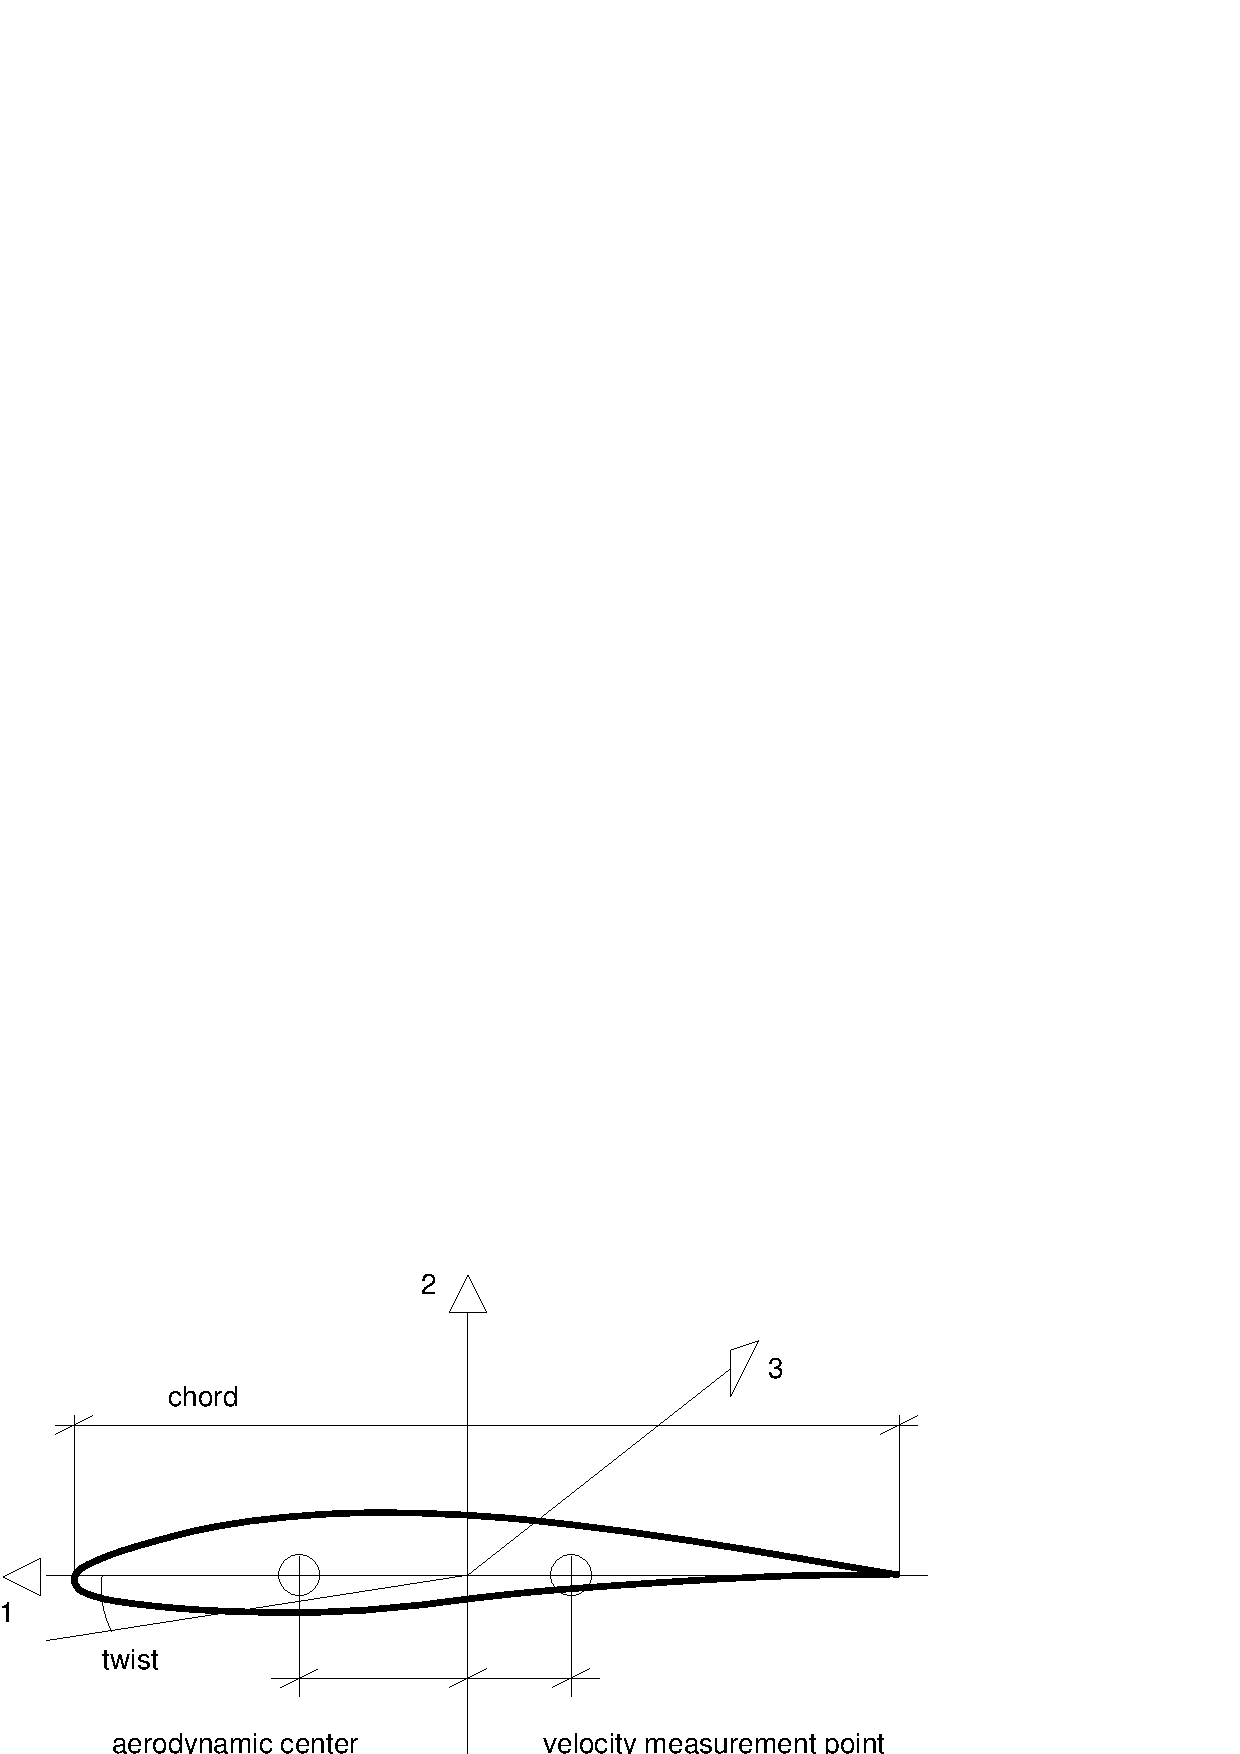
\includegraphics[width=80mm]{airfoil.pdf}
    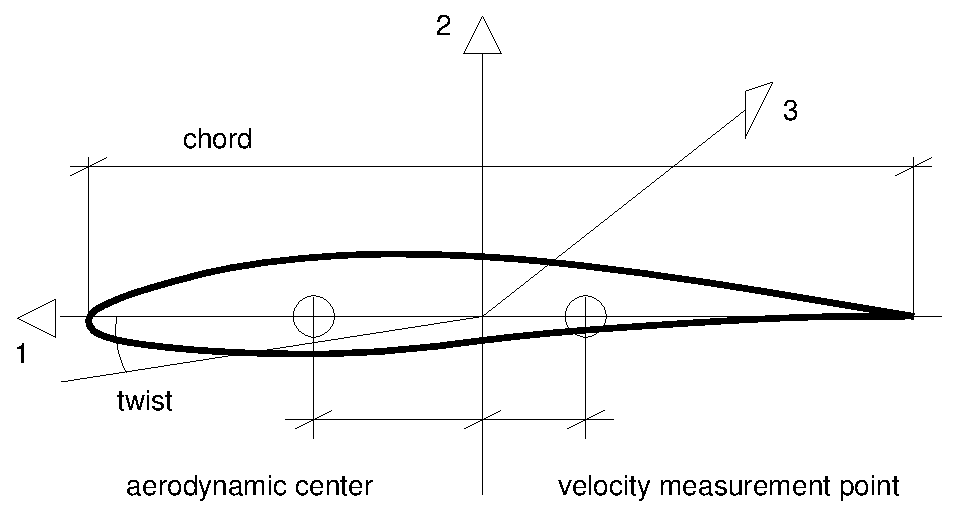
\includegraphics[width=80mm]{airfoil.eps}
  \caption{\em Airfoil Geometry}\label{fig:AIRFOIL}
\end{figure}

The \kw{airfoil\_ data} defaults to a builtin NACA 0012 semi-analytical
model (FIXME: the unsteady correction is buggy; use the \kw{c81} 
mode instead).


\subsection{Output}
Aerodynamic elements, both bodies and beams, write their output with file
extension \kw{.aer}; for each time step the required elements are output.
Three different formats are available; the format can be selected only at
compile time, and it must be the same for all the elements. 

\noindent
\emph{Note: eventually it will freeze; if all the output formats will be
maintained, they will be made selectable at run-time.}

\noindent
In any case the label of the element is output first.

\subsubsection{Node}
The format is:
\begin{itemize}
    \item the label of the node
    \item the three components of the force applied to the node
    \item the three components of the couple applied to the node
\end{itemize}
When an \kw{aerodynamic beam} is considered, the output is repeated 
for each node the element is attached to.

\subsubsection{Forces at Gauss points}
The output refers to each Gauss integration point; the format is:
\begin{itemize}
    \item the direction of the wind velocity relative to the element frame
    \item the lift,
    \item the drag,
    \item and the aerodynamic moment per unit length
\end{itemize}
When an \kw{aerodynamic beam} is considered, the output 
is repeated for each portion of beam.

\subsubsection{Coefficients at Gauss points}
The output refers to each Gauss integration point; the format is:
\begin{itemize}
    \item the local incidence
    \item the local yaw angle
    \item the local Mach number
    \item the lift,
    \item the drag,
    \item and the aerodynamic coefficient
\end{itemize}
When an \kw{aerodynamic beam} is considered, the output 
is repeated for each portion of the beam.





\section{Aircraft instruments}
\begin{verbatim}
    <card> ::= aircraft instruments
    <arglist> ::= <aircraft_node>
\end{verbatim}
The \kw{<aircraft\_node>} represents the aircraft; it is assumed
that the ``nose'' of the aircraft is towards the positive $x$ direction
of the node, and the ``top'' of the aircraft is towards the positive 
$z$ direction of the node.
The available measures are accessed by defining appropriate 
\kw{parameter} nodes, and by binding the \kw{aircraft instruments} 
element private data to the nodes by means of the \kw{bind} mechanism.
The measures are:
\begin{itemize}
	\item \kw{airspeed}
	\item \kw{groundspeed}
	\item \kw{altitude}
	\item \kw{attitude}
	\item \kw{bank}
	\item \kw{turn}
	\item \kw{slip}
	\item \kw{verticalspeed}
	\item \kw{angleofattack}
\end{itemize}

\noindent
\emph{Note: this element is eXperimental.}




\section{Air Properties Element}
The properties of the airstream are made of the physical properties
of the air plus the description of the airstream velocity direction
and amplitude.
The former can be expressed in different forms, while the latter
are based on three-dimensional vectors which depend on multipliers.
\begin{verbatim}
    <arglist> ::= {
        (drive_caller) <air_density> , (scalar) <sound_speed> 
        | std , { { SI | British }
            [ , temperature deviation , <delta T> ]
            | <p0> , (drive_caller) <rho0> ,
            <T0> , <dT/dz> , <R> , <g0> , <z1> , <z2>
        } [ , reference altitude, <z0> ]
    } , (Vec3_tpl_drive_caller) <air_speed>
\end{verbatim}
The first form consists in the bare input of the air density,
in form of a drive caller, and of the sound celerity, e.g.:
\begin{verbatim}
    air properties: 1.225, 340.,
        1.,0.,0., 150.;
\end{verbatim}
The second form uses standard air properties, both in the
international system (SI) or in British units, possibly
with a temperature deviation and an altitude offset, e.g.:
\begin{verbatim}
    air properties: std, SI, temperature deviation, -55,
        reference altitude, 1000.,
        1.,0.,0., 150.;
\end{verbatim}
where standard properties in SI are used, with a temperature
deviation of -55 K degrees and a reference altitude of 1000 m.
The air properties are computed based on the Z position of the
point where the air properties are requested (plus the optional
altitude offset).
The last possibility requires the user to input all the parameters
required to compute the air properties based on the Z position
of the point where they are requested, namely the reference
pressure \kw{p0}, the reference density \kw{rho0},
the reference temperature \kw{T0}, the initial temperature
gradient \kw{dT/dz}, the gas constant \kw{R}, the
initial gravity acceleration \kw{g0}, the bottom and top
altitudes of the null temperature gradient region \kw{z1} and
\kw{z2}; e.g., for SI units:
\begin{verbatim}
    air properties: std,
        101325.,       /* Pa */
        1.2250,        /* kg/m^3 */
        288.16,        /* K */
        -6.5e-3,       /* K/m */
        287.,          /* J/kgK */
        9.81,          /* m/s^2 */
        11000.,        /* m */
        25000.,        /* m */
        temperature deviation, -55,
        reference altitude, 1000.,
        1.,0.,0., 150.;
\end{verbatim}
The asymptotic air properties are characterized by the drive of the 
air speed, in the global reference frame.





\section{Beam Element}
Currently two beam elements are implemented: a three-node finite volume
element, which has been historically implemented first, and uses
conventional polynomial parabolic interpolation of the nodal displacements
and orientations, and a two-node finite volume element, which has been
recently introduced.
Although this latter element presents some shear-locking, it may be overcome
by correcting the section stiffness matrix in a straightforward form:
\begin{displaymath}
	\hat{K} \ = \ \plbr{F + \frac{L^2}{12}T F T^T}^{-1} ,
\end{displaymath}
where $F=K^{-1}$ is the compliance of the section, and
\begin{displaymath}
	T \ = \ \sqbr{\matr{cc}{
		0 & e_x \times{} \\
		0 & 0
	}}
\end{displaymath}
is the ``arm'' matrix that appears in the differential equilibrium equation
\begin{displaymath}
	\vartheta_{/x} - T^T\vartheta + f \ = \ 0 .
\end{displaymath}
The two-node beam will be reimplemented using a helicoidal interpolation
of the nodal positions and orientations, to reduce the shear-locking effect.

\subsection{Three-node beam element}
The beam element is a three node one-dimensional element; it is described 
in detail in \cite{FV-AIAA}.
Each ``node'' is referred to a structural node but can have an arbitrary
offset to allow for more generality in positioning of the structural 
reference lines of the beam.
The ``Finite Volumes'' formulation is used. 
As a consequence, the internal forces and moments are evaluated 
at two points that are at about midpoint between nodes 1 and 2, 
and nodes 2 and 3 (at $ -1/\sqrt{3} $ and $1/\sqrt{3}$ considering
a non-dimensional abscissa running from -1 at node 1 to 1 at node 3).
So the constitutive properties must be supplied in these points, as well as
the orientation matrices from the material to the global frame (the axial force
is in direction 1).
Any of the allowed 6D constitutive laws can be supplied to define the
constitutive properties.
\begin{verbatim}
    <element_type> ::= beam
    <normal_arglist> ::=
        <node_1> , (Vec3) <relative_offset_1> ,
        <node_2> , (Vec3) <relative_offset_2> ,
        <node_3> , (Vec3) <relative_offset_3> ,
        (OrientationMatrix) <orientation_matrix_section_I> ,
        (ConstitutiveLaw6D) <constitutive_law_section_I> ,
        { same | (OrientationMatrix) <orientation_matrix_section_II> } ,
        { same | (ConstitutiveLaw6D) <constitutive_law_section_II> }
\end{verbatim}
Based on the type of constitutive law, the simple or the viscoelastic beam
element is used.
The two keywords \kw{same} respectively mean that the same orientation 
and the same constitutive law defined for the first point will be used 
for the second point. \\
A piezoelectric actuator beam element is available; an arbitrary
linear piezoelectric actuation matrix is required, together with the labels
of the abstract nodes that represent the input signal tensions, as follows:
\begin{verbatim}
    <normal_arglist> ::=
        <node_1> , (Vec3) <relative_offset_1> ,
        <node_2> , (Vec3) <relative_offset_2> ,
        <node_3> , (Vec3) <relative_offset_3> ,
        (OrientationMatrix) <orientation_matrix_section_I> ,
        (ConstitutiveLaw6D) <constitutive_law_section_I> ,
        (OrientationMatrix) <orientation_matrix_section_II> ,
        (ConstitutiveLaw6D) <constitutive_law_section_II>
        piezoelectric actuator , 
        <electrodes_number> ,
        <abstract_node_label_list> ,
        (Mat6xN) <piezoelectric_matrix_I> ,
        { same | (Mat6xN) <piezoelectric_matrix_II> }
\end{verbatim}
where the \kw{abstract\_node\_label\_list} is the list of the labels of the
abstract nodes that represent the electrodes.

\subsection{Two-node beam element}
\begin{verbatim}
    <element_type> ::= beam2
    <normal_arglist> ::=
        <node_1> , (Vec3) <relative_offset_1> ,
        <node_2> , (Vec3) <relative_offset_2> ,
        (OrientationMatrix) <orientation_matrix_section_I> ,
        (ConstitutiveLaw6D) <constitutive_law_section_I>
        [ , piezoelectric actuator , 
        <electrodes_number> ,
        <abstract_node_label_list> ,
        (Mat6xN) <piezoelectric_matrix_I> ]
\end{verbatim}

\subsection{Output}
The output related to beam elements is contained in a file with extension 
\kw{.act}; for each time step, the output of the required beams is
considered.
The internal forces and couples are computed from the interpolated strains
along the beam by means of the constitutive law, at the two evaluation
points. 
The format is:
\begin{itemize}
    \item the label of the beam
    \item the three components of the force at the first evaluation point
    \item the three components of the couple at the first evaluation point
    \item the three components of the force at the second evaluation point
    \item the three components of the couple at the second evaluation point    
\end{itemize}



\section{Bind}\label{sec:EL-BIND}
This is not really an element; it is used to instruct a \kw{parameter node}
about which parameter of an element it is bound to.
The \kw{parameter node} must exist, and the binding element, of type 
\kw{element\_type} and label \kw{element\_label}, must have been already 
defined.
The complete syntax is:
\begin{verbatim}
    <arglist> ::= <element_label> , 
                  <element_type> ,
                  <parameter_node_label> , 
                  { <parameter_index> | name , " <parameter_name> " }
\end{verbatim}
Each element makes a number of parameters available for such binding; a
detailed list will be presented in a future release of the input manual.
The value of \kw{parameter\_index} must be legal, i.e.\ between 1 and the
maximum number of parameters made available by the element.
The alternative form, which will become the default, allows more
friendly definition of the binding.
The name of the parameter depends on the element whose property
is being bound.
A complete listing of the parameters that a parameter node 
can be bound to is not available, since most are added based
on developers' needs.
It is advisable that a mechanism for elements to publish 
what parameters they can make available be devised and implemented.

Example: the parameter node \kw{angle} is bound to the rotation
of a revolute hinge.
\begin{verbatim}
    # ... integrator
    begin: control data;
        structural nodes: 2;
        parameter nodes: 2;
        # ... other control data
    end: control data;

    set: integer node1 = 1000;
    set: integer node2 = 2000;
    set integer angle = 5000;

    begin: nodes;
        structural: node1, dynamic, null, eye, null, null;
        structural: node2, dynamic, null, eye, null, null;
        parameter: angle, element;

        # ... other nodes
    end: nodes;

    begin: elements;
        joint: 1, revolute hinge,
            node1, reference, node, null,
                hinge, reference, node, eye,
            node2, reference, node, null,
                hinge, reference, node, eye;
        bind: 1, 1, joint, angle, string, "rx";

        # ... other elements
    end: elements;
\end{verbatim}




\section{Body}
\begin{verbatim}
    <normal_arglist> ::= <node_label> , 
    { 
      (scalar) <mass> , 
      (Vec3)   <relative_center_of_mass> ,
      (Mat3x3) <inertia_matrix>
      [ , inertial , 
          { node | (OrientationMatrix) <orientation_matrix> } ]
    |
      condense, (integer) <num_masses> ,
          (scalar) <mass> , 
          (Vec3)   <relative_center_of_mass> ,
          (Mat3x3) <inertia_matrix> 
          [ , inertial , 
              { node | (OrientationMatrix) <orientation_matrix> } ]
          [ , ... ]
    }
\end{verbatim}
the \kw{inertia\_matrix} is always referred to the center of mass of the
mass that is being added. It can be rotated locally by means of the extra
\kw{orientation\_matrix} supplied after the (optional) keyword \kw{inertial}.
Otherwise, if the keyword \kw{node} is supplied after the keyword 
\kw{inertial}, the inertia matrix is not rotated at all, since it is
assumed to be already in the node reference frame.
If only one mass is defined, the first method should be used. Otherwise,
many masses can be referred to the same element by means of the keyword
\kw{condense}, followed by the number of expected masses \kw{num\_masses}.
The format of each sub-mass is the same as for the single mass input (actually, 
when \kw{condense} is not supplied, \kw{num\_masses} is assumed to be 1).




\section{Bulk Elements}
The \kw{bulk} element is intended as a sort of NASTRAN's \kw{CELAS} card,
that can be used to apply a stiffness term on an arbitrary degree of freedom.
Extensions are planned to different kind of elements.
The syntax of the \kw{bulk} element is:
\begin{verbatim}
    <normal_arglist> ::= <bulk_type> , <bulk_arglist>
\end{verbatim}
At present only the \kw{stiffness spring} type is available.

\subsection{Stiffness spring}
\begin{verbatim}
    <bulk_type> ::= stiffness spring
    <bulk_arglist> ::= (node_dof) <dof> ,
                       (drive_caller) <stiffness_drive>
\end{verbatim}
The equation related to the desired dof of the linked node is added a
contribution based on the value of the desired degree of freedom (even the
derivative can be used) multiplied times the stiffness. \\
{\em Note: this family of elements has been partially superseded by the
\kw{genel} elements, which allow more generality.}




\section{Couple}
An alias of \kw{force}; see Section~\ref{sec:EL-FORCE}.


\section{Driven Element}
The \kw{driven} type is not an element by itself. It is a wrapper that
masks another element and switches it on and off depending on the (boolean)
value of a drive. It can be used to emulate a variable topology model, where 
some elements simply don't contribute to the residual or to the Jacobian
matrices when their drive has a certain value. Since the drivers can be
arbitrary functions of the time, or other parameters including the value of
any degree of freedom, the driven elements can be ``driven'' in a very
flexible way. Every element can be driven, except those that can be
instantiated once only.
The syntax for a driven element is:
\begin{verbatim}
    <normal_arglist> ::= (drive_caller) <element_driver> ,
        {
            <elem_type> : <elem_label> <elem_normal_arglist> 
        |   
            existing : <elem_type> , <elem_label>
        }
\end{verbatim}
When the first format is used, a normal element is read, instantiated, and
wrapped by the \kw{driven} element wrapper. Note that after the element type,
or after the keyword \kw{existing}, a colon is used as a separator.
This is due for compatibility with the restart module and is not likely 
to be eliminated in the future. 
The label of the element must math that of the driving element given at
the beginning.
When the second format is used, an existing element is sought, and it is
wrapped by a driven element. In this case, no new element is instantiated.
Again the label of the element must match that of the driving element given 
at the beginning. For consistency with the syntax, and for more flexibility,
even when wrapping an existing element it is possible to set at the end the
output flags. This flag will override the previously set one.





\section{Electric Elements}
\kw{electric} elements are those elements that model electric and electronic
devices, dealing with abstract degrees of freedom more than with electric
ones (from the program's point of view they are exactly the same, the
difference is only semantic). The true electric elements, such resistors,
switches and so on, are classified as \kw{electric bulk} elements.
The syntax for \kw{electric} elements is:
\begin{verbatim}
    <normal_arglist> ::= <electric_type> , <electric_arglist>
\end{verbatim}
The \kw{electric} elements implemented at present are:
\begin{itemize}
	\item \kw{accelerometer}
	\item \kw{discrete control}
\end{itemize}
The syntax is described below.

\subsection{Accelerometer}
\begin{verbatim}
    <electric_arglist> ::=
        { translational | rotational } ,
        <struct_node_label> ,
        <abstract_node_label> ,
        (Vec3) <measure_direction>
        [ , position , (Vec3) <position> ]
\end{verbatim}
The \kw{position} is optional; it is meaningless for \kw{rotational}
accelerometers.

\noindent
Legacy element: accelerometer with builtin transfer function
\begin{verbatim}
    <electric_arglist> ::= <struct_node_label> ,
        <abstract_node_label> ,
        (Vec3) <measure_direction> ,
        (scalar) <omega> ,
        (scalar) <tau> ,
        (scalar) <csi> ,
        (scalar) <kappa>	
\end{verbatim}
The label \kw{struct\_node\_label} defines the node whose acceleration 
is being measured; the label \kw{abstract\_node\_label} defines the
\kw{abstract node} that will receive the output signal. 
An \kw{electric node} can be used as well (?).
The transfer function of the accelerometer is:
\begin{displaymath}
    \frac{e_0}{a} = \kw{kappa}\frac{\kw{tau} \ s}{
        \plbr{1+\kw{tau} \ s}
        \plbr{1+2 \ \kw{csi}/\kw{omega} \ s+s^2/\kw{omega}^2}
    }
\end{displaymath}
where $ e_0 $ is the output signal, $ a $ is the input (the acceleration)
and $ s $ is the Laplace variable.

\subsection{Discrete control}
  \begin{verbatim}
    <electric_arglist> ::= <num_outputs> , <num_inputs> , <order> ,
        <control_data> , 
        outputs [ , (node_dof) <output_dofs> [ , ... ] ] ,
        inputs [ , (node_dof) <input_dofs> [ , ... ] ] ,
  \end{verbatim}
  The lists of the output and input dofs follows. The input {\tt
  node\_dof}s don't require the \kw{order} field, since they are simply
  used to compute the control forces, and thus identify an equation.
  The \kw{control\_data} has the following syntax:
  \begin{verbatim}  
        <control_data> ::= <control_type> , <control_arglist>
  \end{verbatim}
  At present only a simple form of control is implemented. Other types
  to come are system identification, both recursive and one-shot, and
  adaptive control, with different models and schemes, all based on 
  Generalized Predictive Control (GPC) and Deadbeat Control.
  The \kw{control} syntax is:
  \begin{verbatim}
    <control_data> ::= control , " <control_matrices_file> "
  \end{verbatim}
  where the file \kw{control\_matrices\_file} must contain the matrices
  $ a_c $, $ b_c $ of the control in plain text (as generated by Matlab, for
  instance): \\
  \begin{tabular}{l}
    $ a_{c1} $, \\
    \ldots,     \\
    $ a_{cp} $, \\
    $ b_{c1} $, \\
    \ldots,     \\
    $ b_{cp} $  \\
  \end{tabular} \\
  where $ p $ is the \kw{order} of the controller and the matrices $ a_c $
  have \kw{num\_inputs} rows and \kw{num\_outputs} columns, while the
  matrices $ b_c $ have \kw{num\_inputs} rows and \kw{num\_inputs} columns.





\section{Force}\label{sec:EL-FORCE}
The \kw{force} element has the following syntax:
\begin{verbatim}
  <normal_arglist> ::= <force_type> , <force_arglist>
\end{verbatim}
where \kw{force\_type} can be \kw{abstract} for an abstract force, or 
\kw{conservative} or \kw{follower} for a structural force. The latter types
apply to a \kw{couple} element, which can be structural only.

\subsection{Output}
The output is discussed accordingly to the types of forces. 
The label of the element is output first in all the cases.

\subsection{Abstract force}
\begin{verbatim}
    <force_type> ::= abstract 
    <force_arglist> ::= (node_dof) <dof> ,
                        (drive_caller) <force_magnitude>
\end{verbatim}
the \kw{dof} field is a normal \kw{node\_dof} but no \kw{order} is required
since the \kw{force} simply applies to the equation related to the node,
regardless of the order.

\subsection{Abstract reaction force}
\begin{verbatim}
    <force_type> ::= abstract internal
    <force_arglist> ::= (node_dof) <dof1> ,
                        (node_dof) <dof2> ,
                        (drive_caller) <force_magnitude>
\end{verbatim}
the \kw{dof1} and \kw{dof2} fields are normal \kw{node\_dof}
but no \kw{order} is required since the \kw{force} simply applies
to the equations related to the nodes, regardless of the order, with
opposite magnitudes.

\subsubsection{Output}
The format is:
\begin{itemize}
    \item the label of the element
    \item the label of the abstract node the force is applied to
	(the first node in case of \kw{abstract internal})
    \item the value of the force
\end{itemize}


\subsection{Structural force}
\begin{verbatim}
    <force_type> ::= { conservative | follower } 
    <force_arglist> ::= <node> , 
                        (Vec3) <relative_direction> ,
                        (Vec3) <relative_arm> ,
                        (drive_caller) <force_magnitude>
\end{verbatim}

\subsection{Structural internal force}
\begin{verbatim}
    <force_type> ::= { conservative | follower } internal
    <force_arglist> ::= <node1> , 
                        (Vec3) <relative_direction> ,
                        (Vec3) <relative_arm1> ,
                        <node2> ,
                        (Vec3) <relative_arm2> ,
                        (drive_caller) <force_magnitude>
\end{verbatim}

\subsubsection{Output}
The format is:
\begin{itemize}
    \item the label of the element
    \item the label of the structural node the force is applied to
    \item the value of the force
    \item the three components of the force
    \item the arm of the force, in the global frame (i.e.\ referred
          to point $ \cubr{0,0,0} $)
\end{itemize}


\subsection{Structural couple}
\begin{verbatim}
    <force_type> ::= { conservative | follower } 
    <force_arglist> ::= <node> ,
                        (Vec3) <relative_direction> ,  
                        (drive_caller) <couple_magnitude>
\end{verbatim}

\subsection{Structural internal couple}
\begin{verbatim}
    <force_type> ::= { conservative | follower } internal
    <force_arglist> ::= <node1> ,
                        (Vec3) <relative_direction> ,  
                        <node2> ,
                        (drive_caller) <couple_magnitude>
\end{verbatim}
i.e.\ the arm is not required. 

\subsubsection{Output}
The format is:
\begin{itemize}
    \item the label of the element
    \item the label of the structural node the couple is applied to
    \item the value of the couple
    \item the three components of the couple
\end{itemize}


\noindent
{\em 
Note: by using a \kw{dof} drive, a simple feedback control can be easily
implemented. \\
A more general force element can be written by using a template drive
that contains both the direction and the amplitude. This will be done in the
future. 
}





\section{Genel Element}
\textsc{Genel} is the compact form for \textsc{Gen}eral \textsc{el}ement.
Those elements that cannot in general be classified in a precise way, 
or are just under development and thus are not collected in a class 
of their own until their configuration is stabilized, usually are
classified as \textsc{Genel}.
The syntax of the \textsc{Genel} elements is:
\begin{verbatim}
    <normal_arglist> ::= <genel_type> , <genel_arglist>
\end{verbatim}

\noindent
The output goes in a file with extension \kw{.gen}; only few elements
actually generate output.

\noindent
At present, the \textsc{Genel} class contains very basic general elements
and some special rotorcraft elements.
The latter could be moved to a more specific class in future releases.

\subsection{Special Rotorcraft \textsc{Genel} Elements}
The special \textsc{Genel} elements include the \kw{swashplate}
and the \kw{rotor trim}.

\subsubsection{Swashplate}
The \kw{swashplate} \textsc{Genel} is used to transform the controls 
of a rotor, in terms of collective and fore/aft and lateral cyclic pitch, 
into the elongations of the actuators that actually move the swash plate.
The syntax of the \kw{swashplate} is:
\begin{verbatim}
    <genel_type> ::= swash plate
    <genel_arglist> ::=
        <collective_abstract_node> 
        [ , limits , <min_collective> , <max_collective> ] ,
        <fore/aft_abstract_node> 
        [ , limits , <min_fore/aft> , <max_fore/aft> ] ,
        <lateral_abstract_node> 
        [ , limits , <min_lateral> , <max_lateral> ] ,
        <actuator_1_abstract_node> ,
        <actuator_2_abstract_node> ,
        <actuator_3_abstract_node> 
        [ , <dynamic_coef> , <cyclic_factor> , <collective_factor> ]
\end{verbatim}
The first three abstract nodes will contain the input values (they can be
actuated by means of abstract forces), and the limits on the ``angles'' can
be easily set. 
The last three nodes will contain the values of the stroke of the actuators.
It is assumed that one of the actuators is behind and the others two are in
front of the rotor, numbered clockwise from the top. 
The limits on the actuators will simply force the value of the control
inputs to remain in the boundaries regardless of the input values.
The last three optional parameters are a dynamic coefficient that is used to
add some dynamics to the actuators' stroke, namely the input variables are
applied a sort of \kw{spring stiffness} \kw{bulk} element, while the
actuators' strokes are applied a transfer function of the first order, namely
$ \alpha\dot{x}+x=f $, where $ \alpha=\kw{dynamic\_coef} $ and $ f $ is
the desired stroke, so the smaller is $ \alpha $, the more the behavior is
static.
The \kw{cyclic\_factor} and the \kw{collective\_factor} parameters are
used to scale the inputs from angles in the desired units to strokes, that
usually are dimensional parameters. The actual strokes are made of the
collective contribution multiplied by \kw{collective\_factor}, and the
cyclic contribution multiplied by \kw{collective\_factor} times 
\kw{cyclic\_factor}.

\subsubsection{Rotor Trim}
The syntax of the \kw{rotor trim} is
\begin{verbatim}
    <genel_type> ::= rotor trim
    <genel_arglist> ::= <rotor_label> ,
        <thrust_node_label> ,
        <longitudinal_moment_node_label> ,
        <lateral_moment_node_label> ,
        (drive_caller) <desired_thrust_coefficient> ,
        (drive_caller) <desired_longitudinal_moment_coefficient> ,
        (drive_caller) <desired_lateral_moment_coefficient> ,
        <rotor_solidity> ,
        <rotor_lock_number> ,
        <rotor_nondimensional_flap_frequency> ,
        <thrust_time_constant> , <moments_time_constant> ,
	<thrust_gain> , <moments_gain>
\end{verbatim}
The \kw{rotor trim} is experimental; it allows to set the controls 
of a generic helicopter, in conjunction with the \kw{swashplate}
element, to asymptotically obtain the desired level of thrust and
moment coefficients.
The corresponding behavior in terms of trim values (flapping angles
and shaft angle) has not been implemented yet.
For details, see \cite{PETERS-TRIM90}.




\subsection{General Purpose Elements}
   
\subsubsection{Clamp}
\begin{verbatim}
    <genel_type> ::= clamp
    <genel_arglist> ::= (node_dof) <clamped_node> ,
                        (drive_caller) <imposed_value>
\end{verbatim}
This element simply forces one arbitrary degree of freedom to assume a value
depending on the drive.

\paragraph{Output}
The format is:
\begin{itemize}
    \item the label of the element
    \item the value of the reaction unknown
\end{itemize}
  
\subsubsection{Distance}
\begin{verbatim}
    <genel_type> ::= distance
    <genel_arglist> ::= (node_dof) <node_1> ,
                        (node_dof) <node_2> ,
                        (drive_caller) <imposed_distance>
\end{verbatim}
This element forces the difference between two arbitrary degrees of freedom
to assume the value dictated by the driver.

\paragraph{Output}
The format is:
\begin{itemize}
    \item the label of the element
    \item the value of the reaction unknown
\end{itemize}
  
  
\subsubsection{Spring}
\begin{verbatim}
    <genel_type> ::= spring
    <genel_arglist> ::= (node_dof) <node_1> ,
                        (node_dof) <node_2> ,
                        (ConstitutiveLaw1D) <const_law>
\end{verbatim}
{\em 
    Note: the constitutive law must be \kw{elastic}, but the \kw{distance}
    genel can apply to arbitrary order degrees of freedom, even between degrees 
    of freedom of different order.
}

\subsubsection{Spring support}
\begin{verbatim}
    <genel_type> ::= spring support
    <genel_arglist> ::= (node_dof) <node> ,                      
                        (ConstitutiveLaw1D) <const_law>
\end{verbatim}
{\em
    Note: the \kw{spring support} must use the \kw{algebraic} value of a 
    \kw{differential} node, but it can use an arbitrary constitutive law,
    i.e.\ an elastic constitutive law for a spring, or a viscous
    constitutive law for a damper, and so on.
}

\subsubsection{Cross spring support}
\begin{verbatim}
    <genel_type> ::= spring support
    <genel_arglist> ::= (node_dof) <row_node> ,                      
                        (node_dof) <col_node> ,                      
                        (ConstitutiveLaw1D) <const_law>
\end{verbatim}
It writes a term depending on the \kw{col\_node} degree of freedom in an
arbitrary manner (given by the \kw{const\_law}) to the 
\kw{row\_node} equation. \\
{\em
    Note: the \kw{cross spring support} must use the \kw{algebraic} value
    of a \kw{differential} node, but can use an arbitrary constitutive law,
    i.e.\ an elastic constitutive law for a spring, or a viscous
    constitutive law for a damper, and so on.
}

\subsubsection{Mass}
\begin{verbatim}
    <genel_type> ::= mass
    <genel_arglist> ::= (node_dof) <node> ,                     
                        (drive_caller) <mass>
\end{verbatim}
{\em
    Note: the mass must use the \kw{algebraic} value of a {\tt
    differential} node. The derivative of the \kw{differential} value of
    the dof is differentiated in a state-space sense, and an inertial driven
    term is applied to the equation related to the dof:
    \begin{eqnarray*}
        m\dot{u} + \ldots & = & f \\
	u - \dot{x} & = & 0
    \end{eqnarray*}
}

\subsubsection{Scalar filter}
\begin{verbatim}
    <genel_type> ::= scalar filter
    <genel_arglist> ::= (node_dof) <output_node> ,
                        (node_dof) <input_node> ,
                        <output_order> [ , <output_coef_list> ] ,
                        <input_order> , <input_coef_list>
                        [ , gain , <gain> ]
\end{verbatim}
This element models a scalar filter of the form
\begin{displaymath}
    A\plbr{s}y = B\plbr{s}u
\end{displaymath}
where $ A $, $ B $ are polynomials of arbitrary order, provided it is
causal, namely the \kw{output\_order} is greater than or equal to 
the \kw{input\_order}.
The polynomial $ A $ is assumed to be monic, so only the coefficients
from 1 to \kw{output\_order} must be input, while all the coefficients 
of polynomial $ B $ are required, i.e.\ from 0 to \kw{input\_order}.
If a gain is supplied, all the coefficients of $ B $ are multiplied by the
gain.

\subsubsection{State space SISO}
\begin{verbatim}
    <genel_type> ::= state space SISO
    <genel_arglist> ::= (node_dof) <output_node> ,
                        (node_dof) <input_node> ,
                        <state_order> ,
                        matrix A , <coefficient_list> ,
                        matrix B , <coefficient_list> ,
                        matrix C , <coefficient_list>
                        [ , matrix D , <coefficient> ]
\end{verbatim}
This element models a scalar (SISO) state space filter of the form
\begin{displaymath}
    \lvvect{ 
        \dot{x} = Ax+Bu \\
	y = Cx+Dx
    }
\end{displaymath}
where $ A $ is a matrix \kw{state\_order}$\times$\kw{state\_order},
$ B $ is a vector \kw{state\_order}$\times$1,
$ C $ is a vector 1$\times$\kw{state\_order},
and $ D $ is scalar, if any.
The matrices are read row-oriented.

\subsubsection{State space MIMO}
\begin{verbatim}
    <genel_type> ::= state space MIMO
    <genel_arglist> ::= <num_outputs> , (node_dof) <output_node_list> ,
                        <num_inputs> , (node_dof) <input_node_list> ,
                        <state_order> ,
                        matrix A , <coefficient_list> ,
                        matrix B , <coefficient_list> ,
                        matrix C , <coefficient_list>
                        [ , matrix D , <coefficient_list> ]
\end{verbatim}
This element models a scalar (SISO) state space filter of the form
\begin{displaymath}
    \lvvect{ 
        \dot{x} = Ax+Bu \\
	y = Cx+Dx
    }
\end{displaymath}
where $ A $ is a matrix \kw{state\_order}$\times$\kw{state\_order},
$ B $ is a matrix \kw{state\_order}$\times$\kw{num\_inputs},
$ C $ is a matrix \kw{num\_outputs}$\times$\kw{state\_order},
and $ D $ is scalar \kw{num\_outputs}$\times$\kw{num\_inputs}.
The matrices are read row-oriented.




\section{Gravity Element}
\begin{verbatim}
    <arglist> ::= (Vec3_tpl_drive_caller) <gravity_acceleration>
\end{verbatim}
the drive of the gravity acceleration, in the global reference frame.




\section{Hydraulic Element}\label{sec:EL-HYDR}
{\em 
    Note: under development \\
    Author: Lamberto Puggelli
}
\begin{verbatim}
    <normal_arglist> ::= <hydr_elem_type> , 
                         <hydr_elem_data>
\end{verbatim}
A detailed input description will be given as soon as it is available. \\
\kw{hydraulic\_element\_data} usually contains information about fluid
properties, which are handled by means of an \kw{hydraulic\_fluid}.
This can be directly inserted, following the syntax described in
Section~\ref{sec:HYDRAULIC-FLUID} preceeded by the keyword \kw{fluid}, or a
previously defined fluid can be recalled by using the keyword 
\kw{reference} followed by the label of the desired fluid.

\subsection{Actuator}
\begin{verbatim}
    <hydr_elem_type> ::= actuator ,
    <hydr_elem_data> ::= <node_1> , <node_2> , 
                         <struct_node_1> , (Vec3) <offset_1> ,
                         <struct_node_2> , (Vec3) <offset_2> ,
                         [ direction , (Vec3) <direction> , ]
                         <area_1> ,
                         <area_2> ,
                         <cylinder_length> ,
                         <hydraulic_fluid_properties_1> ,
                         { same | <hydraulic_fluid_properties_2> }
\end{verbatim}

\subsection{Minor Loss}
\begin{verbatim}
    <hydr_elem_type> ::= minor loss ,
    <hydr_elem_data> ::= <node_1> , <node_2> ,
                         <k12> , <k21> , <area> ,
                         <hydraulic_fluid_properties>
\end{verbatim}

\subsection{Control Valve}
\begin{verbatim}
    <hydr_elem_type> ::= control valve ,
    <hydr_elem_data> ::= <node_1> , <node_2> , <node_3> , <node_4>
                         <area> ,
                         [ loss , <loss_factor> , ]
                         (DriveCaller) <state> ,
                         <hydraulic_fluid_properties>
\end{verbatim}
This element represents a valve that connects
\kw{node\_1} to \kw{node\_2} and \kw{node\_3} to \kw{node\_4}
when \kw{state} is positive and \kw{node\_1} to \kw{node\_3}
and \kw{node\_2} to \kw{node\_4} when \kw{state} is negative,
with area proportional to \kw{area} times the norm of \kw{state}, 
being the latter comprised between $-1$ and $1$.
If \kw{loss\_factor} is defined, it represents the fraction
of area that leaks even when \kw{state} is zero.



\subsection{Dynamic Control Valve}\label{sec:EL-HYDR-DYNAMIC_CONTROL_VALVE}
\begin{verbatim}
    <hydr_elem_type> ::= dynamic control valve ,
    <hydr_elem_data> ::= <node_1> , <node_2> ,
                         <node_3> , <node_4> ,
                         (DriveCaller) <force> ,
                         <initial_displacement> ,
                         <max_displacement> ,
                         <duct_width> ,
                         [ loss , <loss_factor> , ]
                         <valve_diameter> ,
                         <valve_density> ,
                         <displacement> ,
                         <velocity> ,
                         <acceleration> ,
                         <hydraulic_fluid_properties>
\end{verbatim}
This element represents a valve that connects
\kw{node\_1} to \kw{node\_2} and \kw{node\_3} to \kw{node\_4}
when the displacement is positive and \kw{node\_1} to \kw{node\_3}
and \kw{node\_2} to \kw{node\_4} when the displacement is negative,
accounting for the dynamics of the valve body.
The control force \kw{force} is applied to the valve, whose 
geometric and structural properties are described by 
\kw{initial\_displacement}, \kw{max\_displacement},
\kw{duct\_width}, \kw{valve\_diameter} and \kw{valve\_density}.
Again the \kw{loss\_factor}, if defined, represents the fraction
of the area that leaks when the displacement is zero.
Finally, \kw{displacement}, \kw{velocity} and \kw{acceleration}
are the penalty coefficients for displacement, velocity and acceleration
when the maximum stroke is reached.




\subsection{Pressure Flow Control Valve}
\begin{verbatim}
    <hydr_elem_type> ::= pressure flow control valve ,
    <hydr_elem_data> ::= <node_1> , <node_2> ,
                         <node_3> , <node_4> ,
                         <node_5> , <node_6> ,
                         (DriveCaller) <force> ,
                         <initial_displacement> ,
                         <max_displacement> ,
                         <duct_width> ,
                         [ loss , <loss_factor> , ]
                         <valve_diameter> ,
                         <valve_density> ,
                         <displacement> ,
                         <velocity> ,
                         <acceleration> ,
                         <hydraulic_fluid_properties>
\end{verbatim}
Same as Dynamic Control Valve (\ref{sec:EL-HYDR-DYNAMIC_CONTROL_VALVE}),
only the pressures at \kw{node\_5} and \kw{node\_6} are applied
at the sides of the valve body and participate in the force balance.



\section{Joint Element}
Many different joints are available. A first rough classification can be
based on which joints have internal degrees of freedom (the reactions) and
which don't. The latter are flexible joints, that directly add their
stiffness contribution to the dynamic system matrix. From the input point
of view there is no difference between the two classes.
a typical joint entry is made as follows:
\begin{verbatim}
    <normal_arglist> :: = <joint_type> , <joint_arglist>
\end{verbatim}
The output is written to a file with extension \kw{.jnt}.
The output is generally made of a standard part, plus some extra information
depending on the type of joint, which, when available, is described along
with the joint description.
Here the standard part is described:
\begin{itemize}
    \item the label of the joint
    \item the three components of the reaction force in a local reference
    \item the three components of the reaction couple in a local frame
    \item the three components of the reaction force in the global frame
    \item the three components of the reaction couple, rotated into the
          global frame
\end{itemize}
Legal joint types, with relative data, are:




\subsection{Angular acceleration}
\begin{verbatim}
    <joint_type> ::= angular acceleration
    <joint_arglist> ::= <node> , (Vec3) <relative_direction> , 
                        (drive_caller) <acceleration>
\end{verbatim}

\subsection{Angular velocity}
\begin{verbatim}
    <joint_type> ::= angular velocity
    <joint_arglist> ::= <node> , (Vec3) <relative_direction> , 
                        (drive_caller) <velocity>
\end{verbatim}

\subsection{Axial rotation}
\begin{verbatim}
    <joint_type> ::= axial rotation
    <joint_arglist> ::= 
        <node_1> , (Vec3) <relative_offset_1> 
        [ , hinge , 
            (OrientationMatrix) <relative_orientation_matrix_1> ] ,
        <node_2> , (Vec3) <relative_offset_2>
        [ , hinge , 
            (OrientationMatrix) <relative_orientation_matrix_2> ] ,
        (drive_caller) <angular_velocity>
\end{verbatim}
{\em
    Note: this joint forces nodes 1 and 2 to rotate about relative 
    axis 3 with imposed angular velocity.
}

\subsection{Beam slider}
This joint implements a slider, e.g.\ it constrains a structural node 
on a string of three-node beams, as discussed in \cite{SLIDER-AIDAA-2003}.
\begin{verbatim}
    <joint_type> ::= kinematic
    <joint_arglist> ::=
        <slider_node> ,
        (Vec3) <relative_offset> ,
        [ hinge , (OrientationMatrix) <relative_or_mat> ] ,
        [ type , { spherical | classic | spline } , ]
        <beam_number> ,
            <3_node_beam> ,
                { same | (Vec3) <first_node_offset> } ,
    [ hinge , { same | (OrientationMatrix) <first_node_or_mat> ] , }
                (Vec3) <mid_node_offset> ,
    [ hinge , (OrientationMatrix) <mid_node_or_mat> ] ,
                (Vec3) <end_node_offset> ,
    [ hinge , (OrientationMatrix) <end_node_or_mat> ] ,
                [ ... ]
        [ , initial beam , <initial_beam> ]
        [ , initial node, <initial_node> ]
        [ , smearing, <smearing_factor> ]
\end{verbatim}
There are three types of slider:
\begin{itemize}
	\item the \kw{spherical} slider does not constrain
	the orientation of the node;
	\item the \kw{classical} slider does allow rotation
	only about the sliding line;
	\item the \kw{spline} slider constrain the orientation
	of the node.
\end{itemize}
For each node of each beam element, the offset and the orientation
of the slider can be defined; except for the first element, the
offset and the orientation of the first node can be specified using
the keyword \kw{same}, which causes the node to take the same
value of the last node of the previous beam.
The \kw{initial\_beam} and \kw{initial\_node} indices
serve as hints to set the initial contact point of the sliding node.
The \kw{smearing\_factor} determines the (non-dimensional) extension
of the interference segment when the node passes from one segment
to another. % \cite{SLIDER}.



\subsection{Brake}
This element models a wheel brake, i.e.\ a constraint that applies
a frictional internal torque between two nodes about an axis.
The frictional torque depends on the normal force that is applied 
as an external input by means of the same friction models implemented
for regular joints.
\begin{verbatim}
    <joint_type> ::= brake
    <joint_arglist> ::= 
        <node_1> , (Vec3) <relative_offset_1> 
        [ , hinge , 
            (OrientationMatrix) <relative_orientation_matrix_1> ] ,
        <node_2> , (Vec3) <relative_offset_2>
        [ , hinge , 
            (OrientationMatrix) <relative_orientation_matrix_2> ] ,
        friction , <average_radius> , 
                   [ preload , <const_value> , ]
                   <friction_model> , 
                   <shape_function>
\end{verbatim}
The \kw{friction\_data} is undocumented yet.
\emph{Note: a \kw{revolute hinge} between the same two nodes 
must be defined as well, such that the only allowed relative kinematics 
between the two nodes are a rotation about relative axis 3.}


\subsection{Clamp}
\begin{verbatim}
    <joint_type> ::= clamp 
    <joint_arglist> ::= <node>
        [ , position ,
            { node | (Vec3) <absolute_position> } ]
        [ , orientation ,
            { node | (OrientationMatrix) <absolute_orientation_matrix> } ]
\end{verbatim}
\emph{Note: the keyword \kw{node} forces the joint to use
the nodal position and reference frame. Otherwise, they must be entered
in the usual way for these entities} \\
\emph{Note: the default value for \kw{position} and \kw{orientation}
are the position and the orientation of the clamped node.}


\subsection{Coincidence}
not implemented yet, use a \kw{spherical hinge} and a \kw{prismatic} 
instead.

\subsection{Deformable displacement hinge}
\begin{verbatim}
    <joint_type> ::= deformable displacement hinge
    <joint_arglist> ::= 
        <node_1> , (Vec3) <relative_offset_1>
        [ , hinge , (OrientationMatrix) <relative_orientation_matrix_1> ] ,
        <node_2> , (Vec3) <relative_offset_2>
        [ , hinge , (OrientationMatrix) <relative_orientation_matrix_2> ] ,
        (ConstitutiveLaw3D) <const_law>
\end{verbatim}

\subsection{Deformable hinge}
\begin{verbatim}
    <joint_type> ::= deformable hinge
    <joint_arglist> ::= 
        <node_1>
        [ , hinge , (OrientationMatrix) <relative_orientation_matrix_1> ] ,
        <node_2> 
        [ , hinge , (OrientationMatrix) <relative_orientation_matrix_2> ] ,
        (ConstitutiveLaw3D) <const_law>
\end{verbatim}
\emph{Note: this hinge constrains the orientations only.
    It should be used in conjunction with a spherical hinge or any kind of
    joint that constrains the displacements too.}

\subsection{Distance}
\begin{verbatim}
    <joint_type> ::= distance 
    <joint_arglist> ::= <node_1> , 
                        [ position , <relative_offset_1> , ]
                        <node_2> ,
                        [ position , <relative_offset_2> , ]
                        { (drive_caller) <distance> | from nodes }
\end{verbatim}

\noindent
{\em 
    Note: the \kw{relative\_offset\_*} are the distances of each end
    of the joint from the relative nodes in the node reference frame \\
    Both the \kw{distance} and the \kw{distance with offset} joints
    allow for null distance, but the transition from null to non-null
    distance is not smooth at all.
} \\
{\em
    Note: in case the keywords \kw{from nodes} are used, a constant drive
    caller is automatically instantiated for the \kw{distance}. 
    Its value is computed from the initial positions of the nodes;
    if defined, the distance between the offsets is considered. 
} \\
{\em
    Note: the \kw{distance with offset} element is deprecated
    in favor of the \kw{distance} with the new syntax, which
    offers the same capabilities.
}
 


\paragraph{Output}
The extra output is:
\begin{itemize}
    \item the three components of the imposed distance in the global frame
    \item the norm of the imposed distance
\end{itemize}



\subsection{Distance with offset}
This element has been deprecated in favor of the \kw{distance}
element, which now supports offsets.  It may be not supported any more
in the future.



\subsection{Drive hinge}
\begin{verbatim}
    <joint_type> ::= drive hinge
    <joint_arglist> ::= 
        <node_1>
        [ , hinge , (OrientationMatrix) <relative_orientation_matrix_1> ] ,
        <node_2> 
        [ , hinge , (OrientationMatrix) <relative_orientation_matrix_2> ] ,
        (Vec3_tpl_drive_caller) <hinge_orientation>
\end{verbatim}
\emph{Note: this element is eXperimental; now it is more reliable, 
but it is limited to $\nrbr{\tt <hinge\_orientation>} < \pi$}.

\subsection{In line}
\begin{verbatim}
    <joint_type> ::= in line
    <joint_arglist> ::= 
        <node_1> , 
        (Vec3) <relative_line_position> ,
        (Mat3x3) <relative_orientation> ,
        <node_2>
        [ , offset , (Vec3) <relative_offset>]
\end{verbatim}
{\em 
    Note: the \kw{in line} joint supersedes the former note; the orientation
    assumes the sliding line is in direction 3.
}

\subsection{In plane}
\begin{verbatim}
    <joint_type> ::= in plane
    <joint_arglist> ::= 
        <node_1> , 
        (Vec3) <relative_plane_position> ,
        (Vec3) <relative_normal_direction> ,
        <node_2>
        [ , offset , (Vec3) <relative_offset>]
\end{verbatim}
{\em
    Note: to make an in-line joint, use two in-plane joints, with the
    planes that intersect along the desired line. \\
    Note: a \kw{inline} element has been added, which automates the above
    reported procedure.
}

\subsection{Kinematic}
This joint will eventually evolve into a connection with external programs
that impose the entire motion of a node; at present, you can use it
by directly writing code in files \verb;mbdyn/struct/kin.cc; and
\verb;mbdyn/struct/kin.h; that implement the motion you wish to impose.
\begin{verbatim}
    <joint_type> ::= kinematic
    <joint_arglist> ::= 
        <node_1> ,
        (drive_caller) <input>
\end{verbatim}
\emph{Note: this element is eXperimental.}

 \subsection{Linear acceleration}
\begin{verbatim}
    <joint_type> ::= linear acceleration
    <joint_arglist> ::= <node> , (Vec3) <relative_direction> , 
                        (drive_caller) <acceleration>
\end{verbatim}

\subsection{Linear velocity}
\begin{verbatim}
    <joint_type> ::= linear velocity
    <joint_arglist> ::= <node> , (Vec3) <relative_direction> , 
                        (drive_caller) <velocity>
\end{verbatim}

\subsection{Modal}\label{sec:EL-STRUCT-JOINT-MODAL}
\emph{Note: under development \\
    Author: Felice Felippone; \\
    Initial review: Giuseppe Quaranta; \\
    Current review: Pierangelo Masarati.}

\begin{verbatim}
    <joint_type> ::= modal
    <joint_arglist> ::=
        { <reference_modal_node> | clamped
            [ , position , (Vec3)<absolute_position> ]
            [ , orientation , (Mat3x3)<absolute_orientation> ] } ,
        <mode_number> ,
        [ , list, <mode> [ , ... ] ]
        <fem_node_number> 
        [ , no damping 
            | proportional damping , <damping_coef>
            | diag damping , 
                <mode_index> , <mode_damping_coef> 
                [ , ... ] 
        ] , " <fem_data_file> " ,
        [ , origin node , <origin_node> ]
        <interface_nodes_number> ,
            <fem_node_label> ,
                <multibody_label> , (Vec3)<offset_of_FEM_node>
            [ , ... ] ,
        " <output_file_name> "
\end{verbatim}
The \kw{reference\_modal\_node} is a special dynamic structural node 
that is required to handle the rigid body motion of the modal joint.
Its input is completely analogous to that of the \kw{dynamic} structural
nodes, see Section~\ref{sec:NODE-STRUCT}, only the keyword \kw{dynamic} 
must be replaced by \kw{modal}.

\noindent
If no rigid body dynamics is required, e.g.\ if the modal element
is clamped, the \kw{clamped} option can be used, which allows
to set the optional \kw{absolute\_position} 
and \kw{absolute\_orientation}; they default to zero and identity.

\noindent
The mode count in \kw{mode\_number} is not required to match
the number of modes listed in the FEM data file; if a lower number
is given, only the first \kw{mode\_number} modes are used;
moreover, a list of active modes can be given, to use non-consecutive
modes; e.g., to use modes 1, 2, 3 and 6 of a set of 10 modes, use:
\begin{verbatim}
	4, list, 1, 2, 3, 6
\end{verbatim}

\noindent
The origin of the FEM grid is placed either in the position and orientation 
of the modal node, or in the absolute position and orientation 
in case the modal element is clamped, unless the \kw{origin node} 
optional keyword is used.
It defines what FEM node corresponds to the \kw{modal} node,
or what node lies in the absolute position and orientation
for a clamped modal element.

\noindent
The list of matchings between FEM and multibody nodes needs
special care.
The \kw{offset\_of\_FEM\_node} field contains the distance
of the FEM node from the respective multibody node.

\noindent
The \kw{fem\_data\_file} can be generated by NASTRAN, using
the \kw{ALTER} cards provided in directory \kw{etc/modal.d/} 
of the distribution.

The steps of the procedure are as follows:
\begin{enumerate} % procedure

\item prepare a NASTRAN input card deck, made of bulk data,
eigenanalysis properties data and/or static loads (details about 
this phase are currently missing and will be provided in future 
releases of the manual).

\item complete the NASTRAN input file by putting some specific
\kw{ALTER} cards.
In detail:
\begin{enumerate}
\item the file \kw{MBDyn\_NASTRAN\_alter\_1.nas} contains
	\kw{ALTER} definitions for static solutions; appropriate
	loading subcases for each solution must be provided
	in the case control and in the bulk data sections
	of the input file;

	\emph{FIXME: I don't know how to use static shapes only}.

\item the file \kw{MBDyn\_NASTRAN\_alter\_2.nas} contains
	\kw{ALTER} definitions for eigenanalysis solutions;
	an appropriate eigenanalysis method, with the related
	data card must be provided in the case control 
	and in the bulk data sections of the input file;

	\emph{FIXME: I don't know how to use this together
		with static shapes; I only get the normal mode shapes,
		even if the matrices are complete}.

\item the file \kw{MBDyn\_NASTRAN\_alter\_3.nas} contains
	\kw{ALTER} definitions for eigenanalysis solutions;
	an appropriate eigenanalysis method, with the related
	data card must be provided in the case control 
	and in the bulk data sections of the input file;

	\emph{Note: this works; see} \kw{tests/modal/beam.README}.

\end{enumerate}
Exactly one of these files must be included at the very top 
of the NASTRAN input file;
they already include the appropriate \kw{SOL} statement, so the
input file must begin with
\begin{verbatim}
$ Replace '#' below with number that matches your needs
INCLUDE 'MBDyn_NASTRAN_alter_#.nas'
CEND
$... any other executive control and bulk data card
\end{verbatim}
The static solution of case (a: \kw{SOL 101}) and the eigensolution
of case (b: \kw{SOL 103}) need to be performed in sequence; 
if only the eigensolution is to be used, the \kw{ALTER} file 
of case (c: \kw{SOL 103}) must be used.
The static solution of case (a) generates a binary file \kw{mbdyn.stm};
the eigensolutions of cases (b--c) generate two binary files, 
\kw{mbdyn.mat} and \kw{mbdyn.tab}, which, in case (b), include
the static solutions as well.


\item Run NASTRAN.


\item Run the tool \kw{utils/femgen}, which transforms the above binary files
into the \kw{fem\_data\_file}.
The file name is currently requested as terminal input; this is the name 
of the file that will be used in the input model for \kw{mbdyn}.
Conventionally, the \kw{.fem} extension is used.

\end{enumerate} % procedure

\noindent
It is strongly recommended that constrained modal analysis
be used for otherwise free bodies, with the statically 
determined constraint consisting of clamping the FEM node 
that will coincide with \kw{reference\_modal\_node}, and using
the \kw{origin node} to make that point the origin of the FEM frame.

\noindent
\textbf{Note about reference frames:} the coincidence constraint between 
multibody and FEM nodes is written between the local frame 
of the FEM node and the global frame of the multibody node.
As such, the multibody nodes must be oriented as the \kw{modal}
node the \kw{modal} joint refers to, if any, or as the reference
orientation of the \kw{modal} joint, if it is clamped.

\noindent
\textbf{Note about initial assembly:} it is very important that multibody 
and FEM nodes at interfaces are given with a high degree of accuracy,
because the initial assembly procedure of the modal element
does not behave very well (it's on the TODO list with a very low
priority); as a consequence, pay very much attention to the input
of these nodes, until more robust procedures are developed.
One trick is to build models incrementally.
%\begin{itemize}
%\item build the model up to the modal element
%\item find out where a FEM node is going to end out by running
%	mbdyn with \kw{abort after: input}
%\item place the corresponding multibody node exactly in the position
%	indicated by the FEM model output.
%\end{itemize}
Offsets between FEM and multibody nodes should be avoided
unless strictly required.

\noindent
\textbf{Note about the FEM file:}
the format of the \kw{fem\_data\_file} is relatively straightforward;
each data block is commented.
In detail, initial modal displacements and velocities can be added,
if required, by manually editing the file; however this practice
is discouraged, unless strictly required.



\subsection{Plane displacement}\label{sec:EL-STRUCT-JOINT-PLANE_DISPLACEMENT}
This joint allows two nodes to move in the common relative 1--2 plane 
and to rotate about the common relative axis 3.
\begin{verbatim}
    <joint_type> ::= plane displacement
    <joint_arglist> ::= 
        <node_1> , (Vec3) <relative_offset_1> 
        [ , hinge , 
            (OrientationMatrix) <relative_orientation_matrix_1> ] ,
        <node_2> , (Vec3) <relative_offset_2>
        [ , hinge , 
            (OrientationMatrix) <relative_orientation_matrix_2> ]
\end{verbatim}
\emph{Note: this element is temporarily disabled;
combine an \kw{in plane} and a \kw{revolute rotation} joint instead.}

\subsection{Plane displacement pin}
This joint allows a node to move in the relative 1--2 plane 
and to rotate about the relative axis 3 with respect to an absolute point 
and plane.
See also Section~\ref{sec:EL-STRUCT-JOINT-PLANE_DISPLACEMENT}.
\begin{verbatim}
    <joint_type> ::= plane displacement pin
    <joint_arglist> ::= 
        <node> , (Vec3) <relative_offset>
        [ , hinge , 
            (OrientationMatrix) <relative_orientation_matrix> ] ,
        (Vec3) <absolute_pin_position>
        [ , hinge , 
            (OrientationMatrix) <absolute_pin_orientation_matrix> ]
\end{verbatim}
\emph{Note: this element is temporarily disabled;
combine an \kw{in plane} and a \kw{revolute rotation} joint instead,
using a grounded node.}


\subsection{Plane hinge}
This joint has been renamed \kw{revolute hinge}; the old name has been
deprecated and may not be supported in future versions.

\subsection{Plane pin}
This joint has been renamed \kw{revolute pin}; the old name has been
deprecated and may not be supported in future versions.

\subsection{Prismatic}
\begin{verbatim}
    <joint_type> ::= prismatic
    <joint_arglist> ::= 
        <node_1>
        [ , hinge , (OrientationMatrix) <relative_orientation_matrix_1> ] ,
        <node_2> 
        [ , hinge , (OrientationMatrix) <relative_orientation_matrix_2> ] ,    
\end{verbatim}

\subsection{Revolute hinge}
\begin{verbatim}
    <joint_type> ::= revolute hinge
    <joint_arglist> ::= 
        <node_1> , (Vec3) <relative_offset_1> 
        [ , hinge , 
            (OrientationMatrix) <relative_orientation_matrix_1> ] ,
        <node_2> , (Vec3) <relative_offset_2>
        [ , hinge , 
            (OrientationMatrix) <relative_orientation_matrix_2> ]
        [ , friction , <average_radius> , 
                   [ preload , <const_value> , ]
                   <friction_model> , 
                   <shape_function> ]
\end{verbatim}
{\em
    Note: this joint forces nodes 1 and 2 to rotate only about relative 
    axis 3.
}

\subsection{Revolute pin}
\begin{verbatim}
    <joint_type> ::= revolute pin
    <joint_arglist> ::= 
        <node> , (Vec3) <relative_offset>
        [ , hinge , 
            (OrientationMatrix) <relative_orientation_matrix> ] ,
        (Vec3) <absolute_pin_position>
        [ , hinge , 
            (OrientationMatrix) <absolute_pin_orientation_matrix> ]
\end{verbatim}
{\em
    Note: this is the dual of the revolute hinge when one node is grounded.
}

\subsection{Revolute rotation}
A revolute joint without position constraints; this joint, in conjunction
with an \kw{inline} joint, should be used to constrain the two nodes
of a hydraulic actuator.
\begin{verbatim}
    <joint_type> ::= revolute rotation
    <joint_arglist> ::= 
        <node_1>
        [ , hinge , 
            (OrientationMatrix) <relative_orientation_matrix_1> ] ,
        <node_2>
        [ , hinge , 
            (OrientationMatrix) <relative_orientation_matrix_2> ]
\end{verbatim}
{\em
    Note: this joint forces nodes 1 and 2 to rotate only about relative 
    axis 3.
}

\subsection{Rod}
\begin{verbatim}
    <joint_type> ::= rod 
    <joint_arglist> ::= <node_1> , <node_2> , 
        (scalar) { <rod_length> | from nodes }
        [ , offset , (Vec3) <relative_offset_1> , 
                     (Vec3) <relative_offset_2> ] ,
        (ConstitutiveLaw1D) <const_law>
\end{verbatim}
The constitutive law \kw{<const\_law>} is used in form 
of rod axial stiffness $EA$, i.e., for a linear constitutive law:
\begin{displaymath}
	F = EA \frac{l - l_0}{l_0}
\end{displaymath}
and in general
\begin{displaymath}
	F = F\plbr{\frac{l - l_0}{l_0}, \frac{\dot{l}}{l_0}}
\end{displaymath}
where $l_0=\kw{<rod\_length>}$.
For further details on the constitutive laws, 
see Section~\ref{sec:CONSTITUTIVE-LAWS}.
See also \kw{rod with offset} in Section~\ref{sec:EL-STRUCT-JOINT-ROD-WITH-OFFSET}.

\subsection{Rod with offset}\label{sec:EL-STRUCT-JOINT-ROD-WITH-OFFSET}.
\begin{verbatim}
    <joint_type> ::= rod with offset
    <joint_arglist> ::= <node_1> , (Vec3) <relative_offset_1>
                        <node_2> , (Vec3) <relative_offset_2>
        (scalar) { <rod_length> | from nodes } ,
        (ConstitutiveLaw1D) <const_law>
\end{verbatim}
Analogous to \kw{rod} with the optional arg \kw{offset}.

\subsection{Spherical hinge}
\begin{verbatim}
    <joint_type> ::= spherical hinge
    <joint_arglist> ::= 
        <node_1> , (Vec3) <relative_offset_1> 
        [ , hinge , 
            (OrientationMatrix) <relative_orientation_matrix_1> ] ,
        <node_2> , (Vec3) <relative_offset_2>
        [ , hinge , 
            (OrientationMatrix) <relative_orientation_matrix_2> ]
\end{verbatim}
{\em
    Note: the orientation matrix is used for output purposes only. 
    A default identity matrix is assumed.
}

\subsection{Spherical pin}
\begin{verbatim}
    <joint_type> ::= spherical pin
    <joint_arglist> ::= <node> , (Vec3) <relative_offset> ,
                                 (Vec3) <absolute_pin_position>
\end{verbatim}
{\em
    Note: this is the dual of the spherical hinge when one node is grounded.
    An alternative way to model a grounded spherical hinge requires the use
    of a static, clamped node.
}

\subsection{Universal hinge}
\begin{verbatim}
    <joint_type> ::= universal hinge
    <joint_arglist> ::= 
        <node_1> , (Vec3) <relative_offset_1> 
        [ , hinge , 
            (OrientationMatrix) <relative_orientation_matrix_1> ] ,
        <node_2> , (Vec3) <relative_offset_2>
        [ , hinge , 
            (OrientationMatrix) <relative_orientation_matrix_2> ]
\end{verbatim}
{\em
    Note: this joint forces the relative direction 3 of node 1 to be always 
    normal to the relative direction 2 of node 2.
}

\subsection{Universal pin}
\begin{verbatim}
    <joint_type> ::= universal pin
    <joint_arglist> ::= 
        <node> , (Vec3) <relative_offset>
        [ , hinge , 
            (OrientationMatrix) <relative_orientation_matrix> ] ,
        (Vec3) <absolute_pin_position>
        [ , hinge , 
            (OrientationMatrix) <absolute_pin_orientation_matrix> ]
\end{verbatim}
{\em
    Note: this is the dual of the universal hinge when one node is grounded.
}

\subsection{Universal rotation}
A universal joint without position constraints.
\begin{verbatim}
    <joint_type> ::= universal rotation
    <joint_arglist> ::= 
        <node_1>
        [ , hinge , 
            (OrientationMatrix) <relative_orientation_matrix_1> ] ,
        <node_2>
        [ , hinge , 
            (OrientationMatrix) <relative_orientation_matrix_2> ]
\end{verbatim}
{\em
    Note: this joint forces the relative direction 3 of node 1 to be always 
    normal to the relative direction 2 of node 2.
}


\section{Loadable Element}
The \kw{loadable} element is a wrapper for a user-defined element that is
compiled in a separated module and linked run-time.
The module should provide a comprehensive set of functions with a specified
API; default functions are available if no special features are required.
Implementation of modules can be very easy, but a deep knowledge of the
internals of the code is required if special tasks are required. 
There are virtually no limits on what a loadable element can do.
The syntax is simply:
\begin{verbatim}
    <normal_arglist> ::= " <module_name> "
                         [ , name, " <calls> " ] 
                         [ , <module_data> ]
\end{verbatim}
where \kw{module\_name} is the name of the module file; as soon as the file
is checked and the binding of the structure with function bindings 
succeeded, a function called \kw{read} is invoked, and passed the input
stream.
This function is in charge of reading \kw{module\_data} following the
general syntax of the input file.

It is advisable that the function \kw{read} prints some help message
when the first field of \kw{module\_data} is the keyword \kw{help}.
All the helpers and the high-level structures are available, such as
drivers, constitutive laws, reference frames.
Refer to each module for a description (if available) of the features and of
the input/output format.
\kw{module\_name} should be a full path to the module function.
If the name starts with a slash ``/'', the full path name is used.
Otherwise the module is searched in the colon-separated list of directories 
contained in the environment variable \kw{LD\_LIBRARY}, then among the
libraries listed in \kw{/etc/ld.so.cache}, and finally in
\kw{/usr/lib} and in \kw{/lib} (see \kw{dlopen(3)}).
At last, it is searched in the current directory, and the extension
\kw{.so} is added if missing.
The string \kw{<calls>} represents the name of the structure that contains
the bindings to the functions.
The default is \kw{calls}.

\noindent
Refer to \kw{\$(BASE)/mbdyn/base/loadable.h} for a description of the
functions that are allowed.
An example module is given in directory
\begin{verbatim}
    $(BASE)/modules/module-template/
\end{verbatim}
which can be used as a starting point for building a custom module.
% An analogous C/FORTRAN style interface is being planned, at the cost of
% possibly losing some of the fancy C++ features made available by the code.
The \kw{loadable element} interface allows to link modules in different
languages, e.g.\ C or FORTRAN77; simply use \kw{module-template}
as a guideline to providing callbacks to the \kw{loadable element}
interface and to collect required info from the main program
(e.g.\ node positions, equation indices and everything else that is
required for appropriate connection), then call the functions that
actually do the work in other languages from inside the callbacks.
Note that, in general, to call external functions from C++ one needs
to declare them as
\begin{verbatim}
    #include <sys/types.h>
    extern "C" {
        int a_C_function(int arg, double darg);
        int a_F77_subroutine(int32_t *iarg, double *darg);
    }
\end{verbatim}
The same applies to FORTRAN 77 functions; only, the naming convention
usually is compiler dependent; some compilers turn all the names to 
uppercase or lowercase (remember that FORTRAN 77 is case insensitive);
other compilers add underscores at the beginning or at the end of the
names.
Check what is the behavior of your compiler, by compiling a simple 
program with your favorite FORTRAN 77 compiler, then looking at it
with the utility \kw{nm(1)}, which will show how the symbols are represented 
internally.

\noindent
For instance, the code
\begin{verbatim}
C This is a compiler test
      SUBROUTINE F77SUB(I, D)
      INTEGER*4 I
      REAL*8 D(*)

      D(I) = 0.0

      END
\end{verbatim}
when compiled with \kw{g77(1)} on a Linux system, yields:
\begin{verbatim}
[masarati@mbdyn manual]$ g77 -c f77sub.f
[masarati@mbdyn manual]$ nm f77sub.o
00000000 T f77sub_
\end{verbatim}
That is, \kw{g77(1)} lowercases all symbols, and adds a trailing 
underscore.
Macros to automatically detect and take care of this behavior 
will be added.


\noindent
To compile loadable modules, one needs to configure
the package as follows:
\begin{verbatim}
    ./configure --with-module=<module_name>
\end{verbatim}
where \kw{module\_name} is the name of the directory the module
is placed in with the \kw{module-} part stripped; e.g.\ to compile
the tire module that resides in \kw{\$(BASE)/modules/module-wheel2} 
one must type
\begin{verbatim}
    ./configure --with-module=wheel2
\end{verbatim}
Multiple modules can be compiled by typing the list of the names
separated by blanks.
The modules need to resolve some of the symbols that are in the
main executable; until a full working libtool support is implemented,
this must be done by hand.
For the \kw{g++(1)} compiler one requires the switch \kw{-rdynamic} 
to be added to the loader flags, e.g.
\begin{verbatim}
    LDFLAGS="-rdynamic" ./configure --with-module=<module_name>
\end{verbatim}
on \kw{sh(1)} and compatible shells like \kw{bash(1)}, or
\begin{verbatim}
    env LDFLAGS="-rdynamic" ./configure --with-module=<module_name>
\end{verbatim}
on \kw{csh(1)} and compatible shells.





\section{Output Elements}

\subsection{RTAI output}\label{sec:EL-BASE-RTAI_out}
This is a special element which takes care of sending generic output
to external processes by means of RTAI mailboxes during real-time 
simulations.
This topic is under development, so expect frequent changes, and
please do not count too much on backward compatibility.
The syntax is:
\begin{verbatim}
    <normal_arglist> ::=
        name , " <mailbox_name> " ,
        create , { yes | no } ,
        [ host , " <host_name> " , ]
        <channel_number> ,
            (node_dof) <output_dof>
            [ , ... ]
\end{verbatim}
where
\begin{itemize}
\item \kw{<mailbox\_name>} is the name of the RTAI mailbox where 
the output is written  (a unique string not longer than six chars);
\item the \kw{create} keyword determines whether the mailbox
must be created or looked-up as already existing on the system;
\item \kw{<host\_name} is the name or the IP of the remote host where
the mailbox resides; note that if this field is given, \kw{create} must
be set to \kw{no} and the mailbox must be already defined
on the remote host;
\item the number of channels \kw{<channel\_number>} that are written
determines how many \kw{node\_dof} entries must be read.
They must be valid scalar dof entries, which can be connected
in many ways to nodal degrees of freedom or to element private data.
\end{itemize}

\emph{Note: at present, these elements require that the simulation
be run in real-time mode (see Section~\ref{sec:REAL-TIME});
future development will allow to emulate the use of these elements
also when the simulation is not run in real-time, e.g.\ for modeling
or model debugging purposes.}






\subsection{Stream output}\label{sec:EL-BASE-STREAM_OUTPUT}
This is a special element which takes care of sending generic output
to external processes by means of RTAI mailboxes during real-time 
simulations.
This topic is under development, so expect frequent changes, and
please do not count too much on backward compatibility.
The syntax is:
\begin{verbatim}
    <normal_arglist> ::= stream output
        name , " <mailbox_name> " ,
        create , { yes | no } ,
        [ { local , " <socket_name> " , |
            [ port , <port_number> , ]
            [ host , " <host_name> " , ] } ]
        <channel_number> ,
            (node_dof) <output_dof>
            [ , ... ]
\end{verbatim}
The stream output allows MBDyn to send streamed outputs 
to remote processes both during regular simulations and during 
real-time simulations under RTAI.
If the simulation is run in real-time, it uses RTAI mailboxes, 
otherwise regular UNIX sockets are used, either in the \kw{local} or 
in the \kw{internet} namespace.

This output element type is intended to allow the development 
of real-time models by running regular simulations for the purpose 
of debugging the model and the control process without the overhead 
and the potential problems of running in real-time.
Then the same model can be run in real-time without changing the details
of the communication with the controller process.

\paragraph{Non real-time simulation}
During non real-time simulations, streams operate in blocking mode.
The meaning of the parameters is:
\begin{itemize}
\item \kw{<name>} indicates the name the stream
will be known as; it is limited to 6 characters, and mostly useless;
\item the instruction \kw{create} determines whether the socket will be
created or looked for by MBDyn;
\item the keyword \kw{local} indicates that a socket 
in the local namespace will be used; if \kw{create} is set to \kw{yes},
the socket is created, otherwise it must exist.
\item either of the keywords \kw{port} or \kw{host} indicate that a socket
in the internet namespace will be used;
if \kw{create} is set to \kw{yes}, \kw{<host\_name>} indicates 
the host that is allowed to connect to the socket; it defaults 
to any host (\kw{0.0.0.0}); if \kw{create} is set to \kw{no},
\kw{<host\_name>} indicates what host to connect to; the default 
is localhost (\kw{127.0.0.1}); the default port is \kw{5500};
\end{itemize}
If no socket type is specified, i.e.\ none of the \kw{local}, \kw{port} 
and \kw{host} keywords are given, a socket is opened by default 
in the internet namespace with the default IP and port; the \kw{create}
keyword is mandatory.

\paragraph{Real-time simulation}
During real-time simulations, streams wrap non-blocking RTAI mailboxes.
The meaning of the parameters is:
\begin{itemize}
\item the parameter \kw{<name>} indicates the name the stream
will be known as in RTAI's resource namespace; it is limited to 6 characters;
\item the instruction \kw{create} determines whether the mailbox will be
created or looked for by MBDyn;
\item the keyword \kw{local} is ignored;
\item the keyword \kw{host} indicates that a mailbox on a remote host 
will be used; it is useless when \kw{create} is set to \kw{yes}, because
RTAI does not provide the possibility to create remote resources;
if none is given, a local mailbox is assumed;
\item the keyword \kw{port} is ignored.
\end{itemize}

The number of channels \kw{<channel\_number>} that are written
determines how many \kw{node\_dof} entries must be read.
They must be valid scalar dof entries, which can be connected
in many ways to nodal degrees of freedom or to element private data.






\section{Rotor Element}
The \kw{rotor} element is used to associate the aerodynamic elements that
model the blades of a rotor when some inflow related computations are
required. By means of different inflow models, and by means of the
aerodynamic load contributions supplied by the aerodynamic elements, the
rotor element is able to compute the induced velocity at an arbitrary point on
the rotor disk. This velocity term on turn is used by the aerodynamic
elements to determine a better estimate of the boundary conditions.
The syntax of the \kw{rotor} element is:
\begin{verbatim}
    <normal_arglist> ::= <craft_node> ,
            [ hinge , (Mat3x3)<rotor_orientation> , ]
        <rotor_node> ,
        induced velocity , <induced_velocity_model>
\end{verbatim}
The optional \kw{rotor\_orientation} is required when axis 3 
of the \kw{craft\_node} is not aligned with the rotor axis; axis 3
of the \kw{rotor\_node} must be aligned with the rotor axis.

\emph{Note: after the keyword \kw{induced velocity} there used to be
a colon is used as separator.
This changed for uniformity with the rest of the syntax.
No backwards compatibility is provided, so users are urged to update
their models.
A warning is issued.
}

\noindent
There are five models of induced velocity. 
The first is no induced velocity; the syntax is:
\begin{verbatim}
    <induced_velocity_model> ::= no
\end{verbatim}
There is no argument list. This element doesn't compute any induced
velocity, but still computes the rotor traction for output purposes,
if output is required.
The others have a fairly common syntax.  The first three are
\kw{uniform}, \kw{glauert} and \kw{mangler} induced velocity
models:
\begin{verbatim}
    <induced_velocity_model> ::= { uniform | glauert | mangler } , 
        <reference_omega> , <reference_radius> 
        [ , ground , <ground_node> ]
        [ , delay , (drive_caller) <memory_factor> ]
        [ , max iterations , <max_iterations> ]
        [ , tolerance , <tolerance> ]
        [ , eta , <eta> ]
        [ , correction , <hover_correction_factor> ,
            <ff_correction_factor> ]
\end{verbatim}
the \kw{reference\_omega} field is used to decide whether to inhibit
or not the induced velocity computation if the rotor speed is very low;
the \kw{reference\_radius} field is used in the adimensionalization
of the rotor related parameters. \\
The \kw{memory\_factor}, the \kw{hover\_correction\_factor} 
and the \kw{ff\_correction\_factor} (forward flight) are
used to correct the nominal induced velocity, according to the formula
%\begin{eqnarray*}
%	U_{effective} & = &
%	\plbr{1 - \kw{memory\_factor}} 
%		\kw{correction\_factor} \ U_{nominal} \\
%	& & \mbox{} + \kw{memory\_factor} \ U_{previous}
%\end{eqnarray*}
\begin{eqnarray*}
	U_{effective} & = &
	\plbr{1 - \mathtt{<memory\_factor>}} 
		U_{nominal} \\
	& & \mbox{} + \mathtt{<memory\_factor>} \ U_{previous}
\end{eqnarray*}
with
\begin{displaymath}
	U_{nominal} = \frac{T}{2 \rho A V_{tip} \sqrt{
		\cfrac{\lambda^2}{\mathtt{<hover\_correction\_factor>}^4}
		+ \cfrac{\mu^2}{\mathtt{<ff\_correction\_factor>}^2}
	}}
\end{displaymath}
The \kw{memory\_factor} parameter is used to
combine the current reference induced velocity with the induced velocity
at the previous step; no delay means there is no memory of the previous value 
(\emph{Note: for historical reasons, the keyword \kw{weight}
can be used instead of \kw{delay}}). \\
The \kw{memory\_factor} parameter defaults to 0; 
the \kw{hover\_correction\_factor} 
and the \kw{ff\_correction\_factor} parameters default to 1. \\
The \kw{max\_iterations}, the \kw{tolerance} 
and the \kw{eta} parameters refer to the iteration cycle 
that is performed to compute the nominal induced velocity; 
after \kw{max\_iterations}, or when the absolute value 
of the difference between two iterations of the nominal induced 
velocity is less than \kw{tolerance}, the cycle breaks.
Only a fraction \kw{eta} of the difference between two
iterations of the nominal induced velocity is actually
used; \kw{eta} defaults to one.
The default is to make only one iteration, which is backward-compatible
with the original behavior.
\emph{
	Note: the syntax of the correction factor input changed
	from MBDyn 1.1 to MBDyn 1.2, where two different factors,
	according to conventional models (e.g.\ CAMRAD/JA), have
	been considered instead of one.
	No backward compatibility has been implemented because 
	this is a very specialistic parameter and it was introduced 
	very recently.
}

\noindent
The last one uses a dynamic inflow model, based on \cite{PITT},
with inflow states.
The syntax is:
\begin{verbatim}
    <induced_velocity_model> ::= dynamic inflow , 
        <reference_omega> , 
        <reference_radius> 
        [ , ground , <ground_node> ]
        [ , initial value , <const_vel> ,
            <cosine_vel> ,
            <sine_vel> ]
        [ , max iterations , <max_iterations> ]
        [ , tolerance , <tolerance> ]
        [ , eta , <eta> ]
        [ , correction , <hover_correction_factor> ,
            <ff_correction_factor> ]
\end{verbatim}
Most of the entries are the same as for the previous models;
the \kw{delay} optional entry is missing, while the three states, 
corresponding to average, fore-aft and lateral inflow,
can be explicitly initialized by means of the optional 
entry \kw{initial value}.



\section{Miscellaneous}
This section lists some extra cards that do not correspond to any
specific simulation entity, but rather alter the behavior 
of existing entries or cause special operations to be undertaken
during model input.

\subsection{Inertia}
This card causes the equivalent inertia properties of a subset
of elements to be generated.
\begin{verbatim}
    <card> ::= inertia : <label>
        [ , name , " <inertia_name> " ]
        [ , position , (Vec3)<reference_position> ]
        [ , orientation , (Mat3x3)<reference_orientation> ]
        , <type_subset> [ , ... ] ;
        <type_subset> ::= <type> , { all | <label_list> }
        <label_list> ::= <label> [ , <label_list> ]
\end{verbatim}
where \kw{type} currently can only be \kw{body}, although more elements
associated to inertia might participate in the future.
All elements whose labels are listed must exist, and duplicates
are detected and considered errors.
The keyword \kw{all} causes all the elements of type \kw{type} 
to be included in the list.
As a result, each \kw{inertia} entry is logged in the \kw{.log} file
in a self explanatory form, referred both to the \kw{global} 
reference frame and to the reference frame n \kw{reference\_position}
oriented as \kw{reference\_orientation}.



\subsection{Output}
There is an extra card that is used to modify the output behavior of 
elements, analogous to that of the nodes:
\begin{verbatim}
    <card> ::= output : <elem_type> , <elem_list> ;
    <elem_list> ::= <elem_label>  [ , <elem_list> ]
\end{verbatim}
\kw{elem\_type} is a valid element type that can be read 
as card name in the \kw{elements} block.
module.







\bibliographystyle{unsrt}
\bibliography{mybib}


\end{document}
